
%--------------------
 
\chapter{Modelos multiparamétricos}
En este capítulo, discutimos situaciones donde se reuieren estimar simultáneamente más de un parámetro, es decir, los datos que enfrentamos se ajustan a una distrubución de probabilidad que involucre a multiples parámetros, específicamente, se estudiará las siguientes distribuciones
\begin{itemize}
\item la distribución normal univariada que tiene dos parámetros: la media $\theta$ y la varianza $\sigma^2$,
\item la distribución normal normal mutivarianza con vector de medias $\btheta$ y la matriz de varianzas y covarianzas $\bSigma$, y
\item la distribución multinomial cuyo parámetro constituye en el vector de probabilidades $\btheta$.
\end{itemize}

En el contexto de la estimación bayesiana, es necesario hallar la distribución posterior conjunta de estos parámetros, y hallar la estimación mediante: (1) hallar teóricamente la esperanza de la distribución posterior conjunta, ó (2) simular valores de la distribución posterior conjunta, de donde se puede obtener la estimación puntual y por intervalo.

\section{Normal univariada con media y varianza desconocida}

Supongamos que se dispone de realizaciones de un conjunto de variables independientes e idénticamente distribuidos $Y_1,\cdots,Y_n\sim N(\theta,\sigma^2)$, cuando se desconoce tanto la media como la varianza de la distribución, es necesario plantear diversos enfoques y situarse en el más conveniente, según el contexto del problema. En términos de la asignación de las distribuciones previa para $\theta$ y $\sigma^2$ es posible:

\begin{itemize}
\item Suponer que la distribución previa $p(\theta)$ es independiente de la distribución previa $p(\sigma^2)$ y que ambas distribuciones son informativas. 
\item Suponer que la distribución previa $p(\theta)$ es independiente de la distribución previa $p(\sigma^2)$ y que ambas distribuciones son no informativas.
\item Suponer que la distribución previa para $\theta$ depende de $\sigma^2$ y escribirla como $p(\theta \mid \sigma^2)$, mientras que la distribución previa de $\sigma^2$ no depende de $\theta$ y se puede escribir como $p(\sigma^2)$.
\end{itemize}

A continuación, analizamos cada uno de estos planteamientos, y desarrollamos los resultados necesrios para la estimación de $\theta$ y $\sigma^2$.

\subsection{Parámetros independientes}

El primer enfoque que considermos para el análisis de los parámetros de interés $\theta$ y $\sigma^2$ en una distribución normal univariada es suponer que las distribuciones previa de cada uno de los parámetros son independientes pero al mismo tiempo son informativas. \citeasnoun{Gelman03} afirma que este supuesto de independencia es atractivo en problemas para los cuales la información previa para $\theta$ no toma la forma de un número fijo de observaciones con varianza $\sigma^2$. Adicionalmente, este supuesto de independencia es coeherente con el hecho de que en la teoría clásica de estimación los estimadores insesgados de varianza mínima de $\theta$ y $\sigma^2$ son independientes (ver \citeasnoun[Sec.2.4]{Zhang}).

En este orden de ideas, y siguiendo la argumentación del capítulo anterior, la distribución previa para el parámetro $\theta$ es
\begin{equation*}
\theta \sim Normal(\mu,\tau^2)
\end{equation*}

y la distribución previa para el parámetro $\sigma^2$ es
\begin{equation*}
\sigma^2 \sim Inversa-Gamma(n_0/2,n_0\sigma^2_0/2)
\end{equation*}

Asumiendo independencia previa, la distribución previa conjunta resulta estar dada por
\begin{equation}
p(\theta,\sigma^2)\propto (\sigma^2)^{-n_0/2-1}\exp\left\{-\dfrac{n_0\sigma^2_0}{2\sigma^2}\right\}
\exp\left\{-\frac{1}{2\tau^2}(\theta-\mu)^2\right\}
\end{equation}

Una vez que se conoce la forma estructural de la distribución previa conjunta, es posible establecer la distribución posterior conjunta puesto que la verosimilitud de los datos, $p(\mathbf{Y} \mid \theta,\sigma^2)$, está dada por la expresión (\ref{vero_normal}) y
\begin{equation*}
p(\theta,\sigma^2 \mid \mathbf{Y})\propto p(\mathbf{Y} \mid \theta,\sigma^2)p(\theta,\sigma^2)
\end{equation*}

\begin{Res}
La distribución posterior conjunta de los parámetros de interés está dada por
\begin{align}
p(\theta,\sigma^2 \mid \mathbf{Y})&\propto (\sigma^2)^{-(n+n_0)/2-1} \notag \\
&\times
\exp\left\{-\frac{1}{2\sigma^2}\left[n_0\sigma^2_0+(n-1)S^2
                                     +n(\bar{y}-\theta)^2\right]-\frac{1}{2\tau^2}(\theta-\mu)^2\right\}
\end{align}
\end{Res}


\begin{proof}
Tenemos que
\begin{align*}
p(\theta,\sigma^2 \mid \mathbf{Y})&\propto p(\mathbf{Y} \mid \theta,\sigma^2)p(\theta,\sigma^2)\\
&\propto(\sigma^2)^{-n/2}\exp\left\{-\frac{1}{2\sigma^2}\sum_{i=1}^n(y_i-\theta)^2\right\}(\sigma^2)^{-n_0/2-1}\exp\left\{-\dfrac{n_0\sigma^2_0}{2\sigma^2}\right\}
\exp\left\{-\frac{1}{2\tau^2}(\theta-\mu)^2\right\} \\
&=(\sigma^2)^{-(n+n_0)/2-1}\exp\left\{-\frac{1}{2\sigma^2}\left[n_0\sigma^2_0+\sum_{i=1}^n(y_i-\theta)^2\right]-\frac{1}{2\tau^2}(\theta-\mu)^2\right\}\\
&\propto (\sigma^2)^{-(n+n_0)/2-1}\exp\left\{-\frac{1}{2\sigma^2}\left[n_0\sigma^2_0+(n-1)S^2
                                     +n(\bar{y}-\theta)^2\right]-\frac{1}{2\tau^2}(\theta-\mu)^2\right\}
\end{align*}
dond la última expresión se obtiene al sumar y restar $\bar{y}$ dentro de $(y_i-\theta)^2$.
\end{proof}


Nótese que la distribución posterior conjunta no tiene una forma estructural conocida y por lo tanto no es posible realizar el método de integración analítica para obtener una constante de integración \cite{Migon}. Sin embargo, sí es posible obtener las distribuciones condicionales posterior de $\theta$ y de $\sigma^2$, notando que
\begin{align*}
p(\theta \mid \sigma^2,\mathbf{Y})\propto p(\theta,\underbrace{\sigma^2}_{fijo} \mid \mathbf{Y})
\ \ \ \ \ \ \ \ \ \text{y} \ \ \ \ \ \ \ \ \ \
p(\sigma^2 \mid \theta,\mathbf{Y})\propto p(\underbrace{\theta}_{fijo},\sigma^2 \mid \mathbf{Y})
\end{align*}

Es decir, para encontrar la distribución posterior marginal de $\theta$ dado $\sigma^2$, se utiliza la distribución posterior conjunta y los términos que no dependan de $\theta$ se incorporan en la constante de proporcionalidad. El mismo razonamiento se aplica para el parámetro $\sigma^2$.

\begin{Res}
La distribución posterior condicional de $\theta$ es
\begin{equation}\label{Post_theta_Gibbs}
\theta  \mid  \sigma^2,\mathbf{Y} \sim Normal(\mu_n,\tau_n^2)
\end{equation}
En donde las expresiones para $\mu_n$ y $\tau_n^2$ están dadas por \ref{tau_sigma_n}, y la distribución posterior condicional de $\sigma^2$ es 
\begin{equation}\label{Post_Sigma2_Gibbs}
\sigma^2  \mid  \theta,\mathbf{Y} \sim Inversa-Gamma\left(\dfrac{n_0+n}{2},\dfrac{v_0}{2}\right)
\end{equation}
con $v_0=n_0\sigma^2_0+(n-1)S^2+n(\bar{y}-\theta)^2$.
\end{Res}

\begin{proof}
Acudiendo a la distribución posterior conjunta e incorporando los términos que no dependen de $\theta$ en la constante de proporcionalidad, se tiene que
\begin{align*}
p(\theta \mid \sigma^2,\mathbf{Y})&\propto \exp\left\{-\frac{n}{2\sigma^2}(\bar{y}-\theta)^2-\frac{1}{2\tau^2}(\theta-\mu)^2\right\}
\end{align*}
Completando los cuadrados y siguiendo el razonamiento de la demostración del Resultado \ref{Res_pos_theta}, se encuentra una expresión idéntica a la función de distribución de una variable aleatoria con distribución $Normal(\mu_n, \tau^2_n)$. Para la distribución posterior condicional de $\sigma^2$, consultar el resultado \ref{posterior_sigma2}.
\end{proof}

Una vez encontradas las distribuciones posteriores condicionales de $\theta$ y $\sigma^2$, se puede obtener la estimación de estos parámetros métodos de Monte Carlo, específicamente utilizando el muestreo de Gibbs, que puesto en el contexto de este capítulo, se resume en los siguientes pasos:
\begin{enumerate}[(1)]
\item Fijar un valor inicial para $\theta$, lo denotamos por $\theta_{(1)}$
\item Simular un valor de la distribución de $\sigma^2|\theta,\mathbf{Y}$ en \ref{Post_Sigma2_Gibbs} donde el parámetro $v_0$ que depende de $\theta$, debe ser reemplazado por $\theta_{(1)}$ del paso anterior. Este valor simulado se denotará por $\sigma^2_{(1)}$
\item  Simlar un valor de la distribución de $\theta|\sigma^2,\mathbf{Y}$ en \ref{Post_theta_Gibbs} donde en $mu_n$ y $\tau^2_n$ se debe reemplazar $\sigma^2$ por $\sigma^2_{(1)}$. Este valor simulado se denota por $\theta_{(2)}$.
\item Se repite los pasos (2) y (3) hasta completar un número de iteraciones suficientes para alcanzar la convergencia en ambos parámetros
\end{enumerate}

Después de ejecutar el muestreador de Gibbs, eliminar los primeros valores simulados para descartar influencia del valor inicial y posiblemente efectuar el \emph{thinning} para eliminar correlaciones que pueden estar presentes, tenemos los valores finales simulados de $\theta$ y $\sigma^2$, de donde podemos calcular la estimación tomando los promedios respectivos, y calcular intervalos de credibilidad como los percentiles muestrales de los valores simulados. 

En cuanto a la distribución predictiva para una nueva observación $\tilde{y}$, esta está dada por
\begin{equation*}
p(\tilde{y}\mid\mathbf{Y})=\int_0^\infty\int_{-\infty}^\infty p(\tilde{y}\mid\theta,\ \sigma^2)p(\theta,\ \sigma^2\mid\mathbf{Y})d\theta\ d\sigma^2
\end{equation*}

Hallar esta distribución de forma exacta no es fácil, y podemos optar por conocer el comportamiento probabilístico de $\tilde{y}$ por medio de la simulación. Tal como se explicó en el capítulo anterior, se debe simular en primer lugar valores de $\theta$ y de $\sigma^2$ de la distribución posterior $p(\theta,\ \sigma^2\mid\mathbf{Y})$ usando el muestreador de Gibbs y posteriormente se simula valores de $\tilde{y}$ de la distribución $p(\tilde{y}\mid\theta,\ \sigma^2)$. 

Ahora, si se quiere conocer el comportamiento de una nueva muestra aleatoria $Y_1^{*},\cdots,Y_{n^*}^{*}$, lo podemos hacer por medio de la distribución predictiva de la media $\bar{Y}^*$ de la siguiente forma: se debe simular en primer lugar valores de $\theta$ y de $\sigma^2$ de la distribución posterior $p(\theta,\ \sigma^2\mid\mathbf{Y})$ usando el muestreador de Gibbs y posteriormente se simula valores de $\bar{Y}^*$ de la distribución $N(\theta,\frac{\sigma^2}{n^*})$.

\begin{Eje}\label{Eje-Renal}
\citeasnoun{Efronims} consideró un conjunto de datos que muestran la función renal de 157 individuos que se sometieron a una prueba médica exhaustiva en un hospital. Los resultados de la prueba renal están en un intervalo de -6 puntos a 4 puntos. Entre más alto sea el resultado, se concluye que el riñón del individuo es más sano. Nótese que estas pruebas son importantes para predecir el comportamiento de un riñón donado a un paciente con problemas renales. Los datos son extraídos de la siguiente página WEB  (\url{http://statweb.stanford.edu/~ckirby/brad/LSI/datasets-and-programs/datasets.html}) y para este ejemplo sólo se utilizaron los primeros 15 datos del archivo.

En principio, es de interés para el investigador conocer la media y la dispersión de estos datos, para poder analizar a fondo la situación de los pacientes que esperan un transplante.

Dado que se trata de una primera aproximación, se prefiere utilizar distribuciones previas no informativas para los parámetros de la media y varianza. Lo anterior se logra en \verb'JAGS' definiendo las distribuciones previas de \verb"mu ~ dnorm(0,0.001)" y de \verb"tau ~ dgamma(0.001,0.001)" donde \verb"tau" corresponde al parámetro de precisión que resulta ser el inverso de la varianza $\sigma^2$. De esta forma, la distribución previa de $mu$ está centrada en cero, pero con una varianza muy grande al igual que la distribución de la varianza, los cuales representan distribuciones previas no informativas.

El siguiente código en \verb'JAGS' muestra cómo se lleva a cabo la inferencia.

\colorbox{black}{\textcolor{white}{\textbf{Código JAGS}}}
\begin{knitrout}
\definecolor{shadecolor}{rgb}{0.933, 0.933, 0.933}\color{fgcolor}\begin{kframe}
\begin{alltt}
\hlstd{Model} \hlkwb{<-} \hlkwa{function}\hlstd{()\{}
  \hlkwa{for} \hlstd{(i} \hlkwa{in} \hlnum{1}\hlopt{:}\hlstd{n)}
  \hlstd{\{}
    \hlstd{y[i]} \hlopt{~} \hlkwd{dnorm}\hlstd{(theta,tau)}
  \hlstd{\}}
  \hlstd{theta} \hlopt{~} \hlkwd{dnorm}\hlstd{(}\hlnum{0}\hlstd{,}\hlnum{0.001}\hlstd{);}
  \hlstd{sigma} \hlkwb{<-} \hlnum{1}\hlopt{/}\hlkwd{sqrt}\hlstd{(tau)}
  \hlstd{tau} \hlopt{~} \hlkwd{dgamma}\hlstd{(}\hlnum{0.001}\hlstd{,} \hlnum{0.001}\hlstd{)}
\hlstd{\}}

\hlstd{n} \hlkwb{<-} \hlnum{15}
\hlstd{y} \hlkwb{<-} \hlkwd{c}\hlstd{(}\hlnum{1.69045085}\hlstd{,} \hlopt{-}\hlnum{1.41076082}\hlstd{,} \hlopt{-}\hlnum{0.27909483}\hlstd{,} \hlopt{-}\hlnum{0.91387987}\hlstd{,} \hlnum{3.21868429}\hlstd{,} \hlopt{-}\hlnum{1.47282460}\hlstd{,}
       \hlopt{-}\hlnum{0.96524353}\hlstd{,} \hlopt{-}\hlnum{2.45084934}\hlstd{,} \hlnum{1.03838153}\hlstd{,} \hlnum{1.79928679}\hlstd{,} \hlnum{0.97826621}\hlstd{,} \hlnum{0.67463830}\hlstd{,}
       \hlopt{-}\hlnum{1.08665864}\hlstd{,} \hlopt{-}\hlnum{0.00509027}\hlstd{,} \hlnum{0.43708128}\hlstd{)}

\hlstd{Model.data} \hlkwb{<-} \hlkwd{list}\hlstd{(}\hlstr{"y"}\hlstd{,}\hlstr{"n"}\hlstd{)}
\hlstd{Model.param} \hlkwb{<-} \hlkwd{c}\hlstd{(}\hlstr{"theta"}\hlstd{,} \hlstr{"sigma"}\hlstd{)}
\hlstd{Model.inits} \hlkwb{<-} \hlkwa{function}\hlstd{()\{}
  \hlkwd{list}\hlstd{(}\hlstr{"theta"}\hlstd{=}\hlkwd{c}\hlstd{(}\hlnum{0}\hlstd{),} \hlstr{"tau"}\hlstd{=}\hlkwd{c}\hlstd{(}\hlnum{1}\hlstd{))}
\hlstd{\}}

\hlstd{Model.fit} \hlkwb{<-} \hlkwd{jags}\hlstd{(}\hlkwc{data}\hlstd{=Model.data,} \hlkwc{inits}\hlstd{=Model.inits, Model.param,} \hlkwc{n.iter}\hlstd{=}\hlnum{10000}\hlstd{,}
               \hlkwc{n.burnin}\hlstd{=}\hlnum{1000}\hlstd{,} \hlkwc{model.file}\hlstd{=Model)}
\end{alltt}


{\ttfamily\noindent\itshape\color{messagecolor}{\#\# module glm loaded}}\begin{verbatim}
## Compiling model graph
##    Resolving undeclared variables
##    Allocating nodes
## Graph information:
##    Observed stochastic nodes: 15
##    Unobserved stochastic nodes: 2
##    Total graph size: 25
## 
## Initializing model
\end{verbatim}
\begin{alltt}
\hlkwd{print}\hlstd{(Model.fit)}
\end{alltt}
\begin{verbatim}
## Inference for Bugs model at "/var/folders/c3/jvv2xf7j2zv8xh875zp2hly40000gn/T//RtmpTV9tVM/modelb03eb7ead65.txt", fit using jags,
##  3 chains, each with 10000 iterations (first 1000 discarded), n.thin = 9
##  n.sims = 3000 iterations saved
##          mu.vect sd.vect  2.5%   25%    50%   75%   98% Rhat n.eff
## sigma      1.609    0.33  1.12  1.38  1.557  1.78  2.39    1  3000
## theta      0.087    0.43 -0.75 -0.18  0.089  0.36  0.95    1  3000
## deviance  56.179    2.10 54.10 54.68 55.554 56.99 61.84    1  3000
## 
## For each parameter, n.eff is a crude measure of effective sample size,
## and Rhat is the potential scale reduction factor (at convergence, Rhat=1).
## 
## DIC info (using the rule, pD = var(deviance)/2)
## pD = 2.2 and DIC = 58.4
## DIC is an estimate of expected predictive error (lower deviance is better).
\end{verbatim}
\end{kframe}
\end{knitrout}

Después de ejecutar diez mil iteraciones, la salida del anterior código muestra una estimación puntual para la esperanza de $Y$ de 0.089 con un intervalo de credibilidad del 95\% dado por (-0.75, 0.95). Por otro lado, la estimación puntual de la desviación estándar de $Y$ es de 1.557 con un intervalo de credibilidad del 95\% dado por (1.12, 2.39).

A continuación se ilustra el uso de \verb'R' el algoritmo de Gibbs para los datos del ejemplo. Se recalca que se utiliza la librería \verb"MCMCpack" \cite{MCMCpack} para generar las realizaciones de la distribución Inversa-Gamma.

\colorbox{black}{\textcolor{white}{\textbf{Código R}}}
\begin{knitrout}
\definecolor{shadecolor}{rgb}{0.933, 0.933, 0.933}\color{fgcolor}\begin{kframe}
\begin{alltt}
\hlkwd{library}\hlstd{(MCMCpack)}
\end{alltt}


{\ttfamily\noindent\itshape\color{messagecolor}{\#\# Loading required package: MASS}}

{\ttfamily\noindent\itshape\color{messagecolor}{\#\# \#\#\\\#\# \#\# Markov Chain Monte Carlo Package (MCMCpack)}}

{\ttfamily\noindent\itshape\color{messagecolor}{\#\# \#\# Copyright (C) 2003-2016 Andrew D. Martin, Kevin M. Quinn, and Jong Hee Park}}

{\ttfamily\noindent\itshape\color{messagecolor}{\#\# \#\#\\\#\# \#\# Support provided by the U.S. National Science Foundation}}

{\ttfamily\noindent\itshape\color{messagecolor}{\#\# \#\# (Grants SES-0350646 and SES-0350613)\\\#\# \#\#}}\begin{alltt}
\hlstd{y} \hlkwb{<-} \hlkwd{c}\hlstd{(}\hlnum{1.69045085}\hlstd{,} \hlopt{-}\hlnum{1.41076082}\hlstd{,} \hlopt{-}\hlnum{0.27909483}\hlstd{,} \hlopt{-}\hlnum{0.91387987}\hlstd{,} \hlnum{3.21868429}\hlstd{,} \hlopt{-}\hlnum{1.47282460}\hlstd{,}
       \hlopt{-}\hlnum{0.96524353}\hlstd{,} \hlopt{-}\hlnum{2.45084934}\hlstd{,} \hlnum{1.03838153}\hlstd{,} \hlnum{1.79928679}\hlstd{,} \hlnum{0.97826621}\hlstd{,} \hlnum{0.67463830}\hlstd{,}
       \hlopt{-}\hlnum{1.08665864}\hlstd{,} \hlopt{-}\hlnum{0.00509027}\hlstd{,} \hlnum{0.43708128}\hlstd{)}
\hlstd{n} \hlkwb{<-} \hlkwd{length}\hlstd{(y)}

\hlcom{#Parámetros previos de theta}
\hlstd{mu} \hlkwb{<-} \hlnum{0}\hlstd{; tau2} \hlkwb{<-} \hlnum{1000}
\hlcom{#Parámetros previos de sigma2}
\hlstd{a} \hlkwb{<-} \hlnum{0.001}\hlstd{; b} \hlkwb{<-} \hlnum{0.001}

\hlstd{nsim} \hlkwb{<-} \hlnum{10000}
\hlstd{theta.pos} \hlkwb{<-} \hlkwd{rep}\hlstd{(}\hlnum{NA}\hlstd{,nsim)}
\hlstd{sigma2.pos} \hlkwb{<-} \hlkwd{rep}\hlstd{(}\hlnum{NA}\hlstd{,nsim)}

\hlcom{# Valor inicial de theta}
\hlstd{theta.pos[}\hlnum{1}\hlstd{]} \hlkwb{<-} \hlnum{0}

\hlcom{#Parámetros posteriores de sigma2	}
\hlstd{a.n} \hlkwb{<-} \hlstd{a}\hlopt{+}\hlstd{n}\hlopt{/}\hlnum{2}
\hlstd{b.n} \hlkwb{<-} \hlstd{b}\hlopt{+}\hlstd{((n}\hlopt{-}\hlnum{1}\hlstd{)}\hlopt{*}\hlkwd{var}\hlstd{(y)}\hlopt{+}\hlstd{n}\hlopt{*}\hlstd{(}\hlkwd{mean}\hlstd{(y)}\hlopt{-}\hlstd{theta.pos[}\hlnum{1}\hlstd{]))}\hlopt{/}\hlnum{2}
\hlcom{#simulación de la distribución posterior condicional de theta}
\hlstd{sigma2.pos[}\hlnum{1}\hlstd{]} \hlkwb{<-} \hlkwd{rinvgamma}\hlstd{(}\hlnum{1}\hlstd{, a.n, b.n)}

\hlcom{########################}
\hlcom{# Muestreador de Gibbs #}
\hlcom{########################}
\hlkwa{for}\hlstd{(i} \hlkwa{in} \hlnum{2}\hlopt{:}\hlstd{nsim)\{}
  \hlcom{#Parámetros posteriores de theta	}
  \hlstd{tau2.n} \hlkwb{<-} \hlnum{1}\hlopt{/}\hlstd{((n}\hlopt{/}\hlstd{sigma2.pos[i}\hlopt{-}\hlnum{1}\hlstd{])}\hlopt{+}\hlstd{(}\hlnum{1}\hlopt{/}\hlstd{tau2))}
  \hlstd{mu.n} \hlkwb{<-} \hlstd{tau2.n}\hlopt{*}\hlstd{(}\hlkwd{mean}\hlstd{(y)}\hlopt{*}\hlstd{(n}\hlopt{/}\hlstd{sigma2.pos[i}\hlopt{-}\hlnum{1}\hlstd{])}\hlopt{+}\hlstd{mu}\hlopt{/}\hlstd{tau2)}
  \hlcom{#simulación de la distribución posterior condicional de theta}
  \hlstd{theta.pos[i]} \hlkwb{<-} \hlkwd{rnorm}\hlstd{(}\hlnum{1}\hlstd{,} \hlkwc{mean}\hlstd{=mu.n,} \hlkwc{sd}\hlstd{=}\hlkwd{sqrt}\hlstd{(tau2.n))}
  \hlcom{#Parámetros posteriores de sigma2	}
  \hlstd{a.n} \hlkwb{<-} \hlstd{a}\hlopt{+}\hlstd{n}\hlopt{/}\hlnum{2}
  \hlstd{b.n} \hlkwb{<-} \hlstd{b}\hlopt{+}\hlstd{((n}\hlopt{-}\hlnum{1}\hlstd{)}\hlopt{*}\hlkwd{var}\hlstd{(y)}\hlopt{+}\hlstd{n}\hlopt{*}\hlstd{(}\hlkwd{mean}\hlstd{(y)}\hlopt{-}\hlstd{theta.pos[i]))}\hlopt{/}\hlnum{2}
  \hlcom{#simulación de la distribución posterior condicional de theta}
  \hlstd{sigma2.pos[i]} \hlkwb{<-} \hlkwd{rinvgamma}\hlstd{(}\hlnum{1}\hlstd{, a.n, b.n)}
\hlstd{\}}
\hlkwd{par}\hlstd{(}\hlkwc{mfrow}\hlstd{=}\hlkwd{c}\hlstd{(}\hlnum{1}\hlstd{,}\hlnum{2}\hlstd{))}
\hlkwd{acf}\hlstd{(theta.pos[}\hlnum{1001}\hlopt{:}\hlstd{nsim])}
\hlkwd{acf}\hlstd{(sigma2.pos[}\hlnum{1001}\hlopt{:}\hlstd{nsim])}
\end{alltt}
\end{kframe}
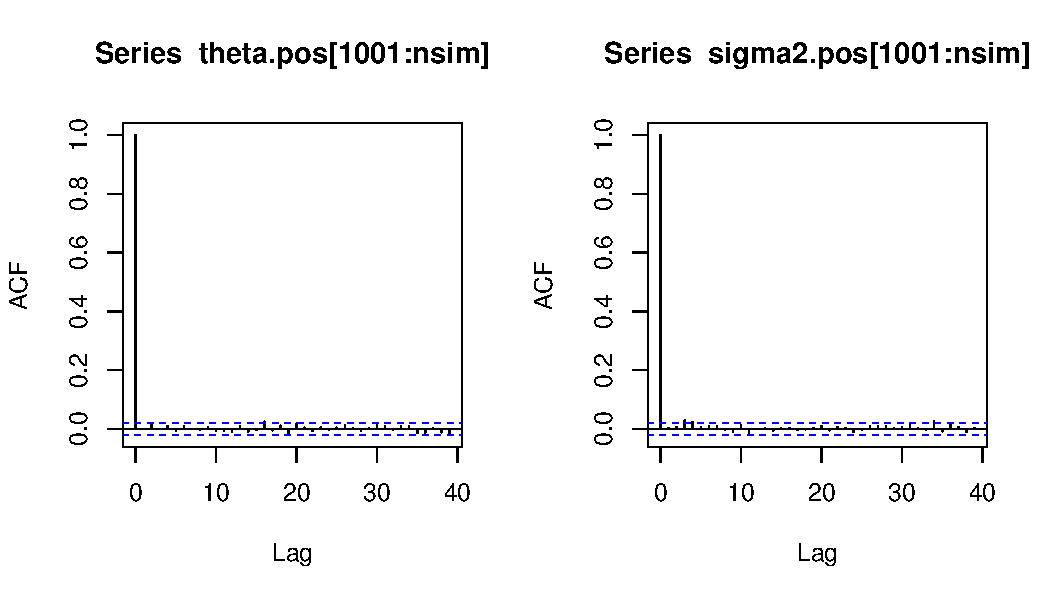
\includegraphics[width=\maxwidth]{figure/unnamed-chunk-3-1} 

\end{knitrout}
Al observar que no existen correlaciones importantes en los valores simulados de $\theta$ y $\sigma^2$ (después de descartar las primeras 1000 iteraciones), se concluye que se puede utilizar directamente estos valores para la obtención de las estimaciones. Por cual, se calcula el promedio y los percentiles muestrales de los valores simulados de la siguiente forma:
\begin{knitrout}
\definecolor{shadecolor}{rgb}{0.933, 0.933, 0.933}\color{fgcolor}\begin{kframe}
\begin{alltt}
\hlkwd{mean}\hlstd{(theta.pos[}\hlnum{1001}\hlopt{:}\hlstd{nsim])}
\end{alltt}
\begin{verbatim}
## [1] 0.085
\end{verbatim}
\begin{alltt}
\hlkwd{quantile}\hlstd{(theta.pos[}\hlnum{1001}\hlopt{:}\hlstd{nsim],} \hlkwd{c}\hlstd{(}\hlnum{0.025}\hlstd{,}\hlnum{0.975}\hlstd{))}
\end{alltt}
\begin{verbatim}
##  2.5%   98% 
## -0.73  0.89
\end{verbatim}
\begin{alltt}
\hlkwd{mean}\hlstd{(}\hlkwd{sqrt}\hlstd{(sigma2.pos[}\hlnum{1001}\hlopt{:}\hlstd{nsim]))}
\end{alltt}
\begin{verbatim}
## [1] 1.5
\end{verbatim}
\begin{alltt}
\hlkwd{quantile}\hlstd{(}\hlkwd{sqrt}\hlstd{(sigma2.pos[}\hlnum{1001}\hlopt{:}\hlstd{nsim]),} \hlkwd{c}\hlstd{(}\hlnum{0.025}\hlstd{,}\hlnum{0.975}\hlstd{))}
\end{alltt}
\begin{verbatim}
## 2.5%  98% 
##  1.0  2.3
\end{verbatim}
\end{kframe}
\end{knitrout}

De donde podemos concluir que una estimación puntual para la esperanza de $Y$ de 0.085 con un intervalo de credibilidad del 95\% dado por (-0.73, 0.89). Por otro lado, la estimación puntual de la desviación estándar de $Y$ es de 1.5 con un intervalo de credibilidad del 95\% dado por (1.0, 2.3), resultados muy similares a lo obtenido don \verb'JAGS'. 

Finalmente ilustramos la forma de obtener la distribución predictiva para el promedio muestral de 5 nuevos pacientes. 
\begin{knitrout}
\definecolor{shadecolor}{rgb}{0.933, 0.933, 0.933}\color{fgcolor}\begin{kframe}
\begin{alltt}
\hlstd{n.ast} \hlkwb{<-} \hlnum{5}\hlstd{; y.bar} \hlkwb{<-} \hlkwd{c}\hlstd{()}
\hlkwa{for}\hlstd{(i} \hlkwa{in} \hlnum{1}\hlopt{:}\hlstd{(nsim}\hlopt{/}\hlnum{2}\hlstd{))\{}
  \hlstd{y.bar[i]} \hlkwb{<-} \hlkwd{rnorm}\hlstd{(}\hlnum{1}\hlstd{,theta.pos[i}\hlopt{+}\hlstd{nsim}\hlopt{/}\hlnum{2}\hlstd{],}\hlkwd{sqrt}\hlstd{(sigma2.pos[i}\hlopt{+}\hlstd{nsim}\hlopt{/}\hlnum{2}\hlstd{]}\hlopt{/}\hlstd{n.ast))}
\hlstd{\}}
\hlkwd{hist}\hlstd{(y.bar)}
\end{alltt}
\end{kframe}
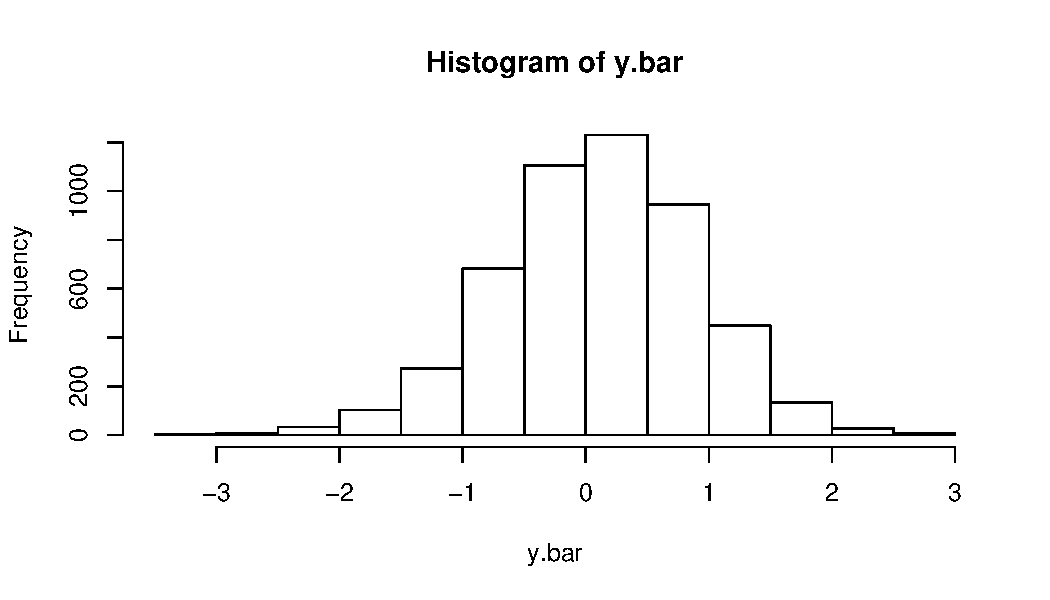
\includegraphics[width=\maxwidth]{figure/unnamed-chunk-5-1} 
\begin{kframe}\begin{alltt}
\hlkwd{mean}\hlstd{(y.bar)}
\end{alltt}
\begin{verbatim}
## [1] 0.097
\end{verbatim}
\begin{alltt}
\hlkwd{sd}\hlstd{(y.bar)}
\end{alltt}
\begin{verbatim}
## [1] 0.8
\end{verbatim}
\begin{alltt}
\hlkwd{quantile}\hlstd{(y.bar,}\hlkwd{c}\hlstd{(}\hlnum{0.025}\hlstd{,}\hlnum{0.975}\hlstd{))}
\end{alltt}
\begin{verbatim}
## 2.5%  98% 
## -1.6  1.6
\end{verbatim}
\end{kframe}
\end{knitrout}
Podemos ver que se espera que el promedio de las pruebas en 5 nuevos pacientes es de 0.097, con un intervalo del 95\% de (-1.6, 1.6), este intervalo es mucho más ancho que el de $\theta$, pues naturalmente $\bar{Y}$ tiene mayor incertidumbre que los parámetros del modelo, y en segundo lugar, el nuevo de nuevos datos es de 5 que es bastante pequeño, lo cual hace que el pronóstico para $\bar{Y}^*$ no sea muy preciso.
\end{Eje}

\subsection{Parámetros dependientes}

En algunas situaciones es muy útil asumir una distribución previa conjugada, y para lograr eso no es posible establecer que los parámetros tengan distribuciones previa independientes. Bajo esta situación, la inferencia posterior de los parámetros de interés debe ser llevada a cabo en dos etapas: En la primera, se debe establecer la distribución previa conjunta para ambos parámetros siguiendo la sencilla regla que afirma que
\begin{equation*}
p(\theta,\sigma^2)=p(\sigma^2)p(\theta \mid \sigma^2)
\end{equation*}

En la segunda etapa ya es posible analizar posterior propiamente cada uno de los parámetros de interés siguiendo otra sencilla regla que afirma que
\begin{equation*}
p(\theta,\sigma^2 \mid \mathbf{Y})\propto p(\mathbf{Y} \mid \theta,\sigma^2)p(\theta,\sigma^2)
\end{equation*}

La anterior formulación conlleva a asignar una distribución previa para $\theta$ dependiente del parámetro $\sigma^2$. Esto quiere decir que en la distribución $p(\theta \mid \sigma^2)$, el valor de $\sigma^2$ se considera una constante fija y conocida, esta distribución previa está dada por\footnote{La forma como la distribución previa de $\theta$ dependa de $\sigma^2$ es coherente con la información de Fisher sobre $\theta$ que es igual a $\sigma^{-2}$.}
\begin{equation*}
p(\theta \mid \sigma^2)\sim Normal(\mu,\sigma^2/c_0)
\end{equation*}

donde $c_0$ es una constante. Por otro lado, y siguiendo los argumentos de la sección 2.7, una posible opción para la distribución previa de $\sigma^2$, que no depende de $\theta$, corresponde a
\begin{equation*}
p(\sigma^2)\sim Inversa-Gamma(n_0/2,n_0\sigma^2_0/2)
\end{equation*}

De esta forma, podemos encontrar la distribución conjunta previa de $\theta$ y $\sigma^2$ como sigue:
\begin{Res}
La distribución conjunta previa de los parámetros $\theta$ y $\sigma^2$ está dada por una distribución
\begin{equation*}
\theta,\sigma^2 \sim Normal-Inversa-Gamma\left(\mu, c_0, \frac{n_0+1}{2},\frac{n_0\sigma^2_0}{2}\right).
\end{equation*}
\end{Res}

\begin{proof}
\begin{align*}
p(\theta,\sigma^2)&=p(\sigma^2)p(\theta \mid \sigma^2)\\
&\propto (\sigma^2)^{-\frac{n_0}{2}-1}\exp\left\{-\dfrac{n_0\sigma_0^2}{2\sigma^2}\right\}
(\sigma^2)^{-\frac{1}{2}}\exp\left\{-\frac{c_0}{2\sigma^2}(\theta-\mu)^2\right\}\\
&= (\sigma^2)^{-\frac{n_0+1}{2}-1}\exp\left\{-\frac{1}{2\sigma^2}\left[n_0\sigma^2_0+c_0(\theta-\mu)^2\right]\right\}
\end{align*}
la cual corresponde a la forma de la función de densidad de la distribución Normal-Inversa-Gamma.
\end{proof}

Una vez encontrada la distribución conjunta previa, procedemos a encontrar la distribución conjunta posterior, y así poder encontrar las estimaciones de $\theta$ y $\sigma^2$.
\begin{Res}
La distribución posterior conjunta de los parámetros $\theta$ y $\sigma^2$ está dada por
\begin{equation*}
\theta,\sigma^2\mid\mathbf{Y} \sim Normal-Inversa-Gamma\left(\mu_n, c_0+n, \frac{n_0+n+1}{2},\beta\right).
\end{equation*}

con 
\begin{equation*}
\beta=\dfrac{1}{2}\left(n_0\sigma^2_0+(n-1)S^2+\dfrac{c_0n}{c_0+n}(\mu-\bar{y})^2\right)
\end{equation*}

y
\begin{equation*}
\mu_n=\frac{\frac{n}{\sigma^2}\bar{Y}+\frac{c_0}{\sigma^2}\mu}{\frac{n}{\sigma^2}+\frac{c_0}{\sigma^2}}
=\frac{n\bar{Y}+c_0\mu}{n+c_0}
\end{equation*}
\end{Res}

\begin{proof}
En primer lugar, recordamos que la función de verosimilitud de la muestra está dada por
\begin{align}
p(\mathbf{Y} \mid \theta,\sigma^2)= \frac{1}{(2\pi\sigma^2)^{n/2}}
\exp\left\{-\frac{1}{2\sigma^2}\left[(n-1)S^2+n(\bar{y}-\theta)^2\right]\right\}
\end{align}
Por otro lado, se tiene que
\begin{align}\label{desarro1}
p(\theta,\sigma^2 \mid \mathbf{Y}) & \propto p(\mathbf{Y} \mid \theta,\sigma^2)p(\theta,\sigma^2)\notag\\
&\propto (\sigma^2)^{-\frac{n_0+n+1}{2}-1}
\exp\left\{-\frac{1}{2\sigma^2}\left[n_0\sigma^2_0+c_0(\theta-\mu)^2+(n-1)S^2+n(\bar{y}-\theta)^2\right]\right\}\notag\\
&= (\sigma^2)^{-\frac{n_0+n+1}{2}-1}\\
&\times
\exp\left\{-\frac{1}{2\sigma^2}\left[n_0\sigma^2_0+(n-1)S^2+(c_0+n)(\theta-\mu_n)^2+\frac{c_0n}{c_0+n}(\mu-\bar{y})^2\right]\right\}
\end{align}
puesto que
\begin{align*}
c_0(\theta-\mu)^2+n(\bar{y}-\theta)^2=(c_0+n)(\theta-\mu_n)^2+\frac{c_0n}{c_0+n}(\mu-\bar{y})^2
\end{align*}
\end{proof}

Para encontrar las distribuciones marginales posterior de cada uno de los parámetros de interés se utilizan argumentos distintos puesto que $\theta$ depende de $\sigma^2$ pero este último no depende del primero. De esta manera se tiene que:
  
\begin{enumerate}
\item Para hallar la distribución posterior condicional de $\theta \mid \sigma^2$, dada por $P(\theta \mid \sigma^2,\mathbf{Y})$, se debe considerar que $\sigma^2$ es una constante fija y conocida tal como se consideró al principio de esta sección. Basado en lo anterior, es posible utilizar la siguiente regla de probabilidad
\begin{align*}
P(\theta \mid \sigma^2,\mathbf{Y})=\frac{p(\theta,\sigma^2 \mid \mathbf{Y})}{p(\sigma^2,\mathbf{Y})}p(\mathbf{Y})\propto p(\theta,\sigma^2 \mid \mathbf{Y})
\end{align*}
Lo anterior sugiere que la distribución marginal posterior de $\theta$, $p(\theta \mid \sigma^2,\mathbf{Y})$, se encuentra utilizando la distribución posterior conjunta, $p(\theta,\sigma^2 \mid \mathbf{Y})$, suponiendo que todas las expresiones que involucren al valor $\sigma^2$ se pueden incluir en la constante de proporcionalidad
\item Dado que $\sigma^2$ no depende de ningún otro parámetro entonces, utilizando la distribución posterior conjunta, es posible encontrar su distribución marginal posterior de la siguiente forma
\begin{align*}
p(\sigma^2 \mid \mathbf{Y})=\int p(\theta,\sigma^2 \mid \mathbf{Y}) d\theta
\end{align*}
Lo propio es posible hacer con $\theta$, utilizando la distribución posterior conjunta, es posible encontrar su distribución marginal posterior de la siguiente forma
\begin{align*}
p(\theta \mid \mathbf{Y})=\int p(\theta,\sigma^2 \mid \mathbf{Y}) d\sigma^2
\end{align*}
\end{enumerate}

\begin{Res}
La distribuciónposterior de $\theta$ condicional a $sigma^2,\sigma^2,\mathbf{Y}$ está dada por
\begin{equation*}
\theta \mid \sigma^2,\mathbf{Y} \sim Normal(\mu_n,\sigma^2/(n+c_0))
\end{equation*}
con $\mu_n=\dfrac{n\bar{y}+c_0\mu}{n+c_0}$.
\end{Res}

\begin{proof}
Acudiendo a la distribución posterior conjunta dada en \ref{desarro1}, tenemos que
\begin{align*}
p(\theta \mid \sigma^2,\mathbf{Y})&\propto 
p(\theta,\sigma^2 \mid \mathbf{Y}) \\
&\propto(\sigma^2)^{-\frac{n_0+n+1}{2}-1}\\
&\hspace{1cm}\times
\exp\left\{-\frac{1}{2\sigma^2}\left[n_0\sigma^2_0+(n-1)S^2+(c_0+n)(\theta-\mu_n)^2+\frac{c_0n}{c_0+n}(\mu-\bar{y})^2\right]\right\}\\
&\propto \exp\left\{-\frac{1}{2\sigma^2}(c_0+n)(\theta-\mu_n)^2\right\}
\end{align*}
la cual corresponde a la forma de la función de densidad de la distribución $Normal(\mu_n, \sigma^2/(n+c_0))$.
\end{proof}

En el anterior resultado, la media de la distribución condicional posterior $\mu_n$ se puede escribir como $\mu_n=\frac{n}{n+c_0}\bar{y}+\frac{c_0}{n+c_0}\mu$, promedio ponderado entre la estimación clásica $\bar{y}$ y la estimación previa $\mu$. Observando la forma que toman los pesos $\frac{n}{n+c_0}$ y $\frac{c_0}{n+c_0}$, se puede pensar a $c_0$ como el número de observaciones en la información previa, y así, los pesos de la estimación clásica y la estimación previa dependen directamente de los tamaños muestrales respectivos.

\begin{Res}\label{Poster_sigma2_IG}
La distribución marginal posterior del parámetro $\sigma^2$ es
\begin{equation*}
\sigma^2 \mid \mathbf{Y} \sim Inversa-Gamma\left(\frac{n+n_0}{2},\frac{(n+n_0)\sigma^2_n}{2}\right)
\end{equation*}
Donde $(n+n_0)\sigma^2_n=n_0\sigma^2_0+(n-1)S^2+\frac{c_0n}{c_0+n}(\mu-\bar{y})^2$ corresponde a una suma ponderada de la varianza previa, la varianza muestral y la distancia entre la media muestral y la media previa.
\end{Res}

\begin{proof}
De la distribución posterior conjunta (3.1.5) e integrando con respecto a $\theta$, se tiene que
\begin{align*}
p(\sigma^2 \mid \mathbf{Y})&=\int p(\theta,\sigma^2 \mid \mathbf{Y}) \ d\theta\\
&\propto (\sigma^2)^{-\frac{n_0+n+1}{2}-1}
\exp\left\{-\frac{1}{2\sigma^2}\left[n_0\sigma^2_0+(n-1)S^2+\frac{c_0n}{c_0+n}(\mu-\bar{y})^2\right]\right\}\\
&\hspace{2cm}\times
\int_{-\infty}^{\infty}\exp\left\{-\frac{n+c_0}{2\sigma^2}(\theta-\mu_n)^2\right\} \ d\theta\\
&\propto (\sigma^2)^{-\frac{n_0+n}{2}-1}
\exp\left\{-\frac{1}{2\sigma^2}\left[n_0\sigma^2_0+(n-1)S^2+\frac{c_0n}{c_0+n}(\mu-\bar{y})^2\right]\right\}\\
&\hspace{2cm}\times
\int_{-\infty}^{\infty}\frac{\sqrt{n+c_0}}{\sqrt{2\pi\sigma^2}}
\exp\left\{-\frac{n+c_0}{2\sigma^2}(\theta-\mu_n)^2\right\} \ d\theta\\
&\propto (\sigma^2)^{-\frac{n_0+n}{2}-1}
\exp\left\{-\frac{(n+n_0)\sigma^2_n}{2\sigma^2}\right\}
\end{align*}
la cual corresponde a la forma de la función de densidad de la distribución $Inversa-Gamma(\frac{n+n_0}{2},\frac{(n+n_0)\sigma^2_n}{2})$.
\end{proof}

Dadas las distribuciones $p(\sigma^2\mid \mathbf{Y})$ y $p(\theta\mid \sigma^2, \mathbf{Y})$, podemos proceder de la siguiente forma para obetener valores simulados de $\theta$ y $\sigma^2$ y de esta forma, obtener las estimaciones. Si el número de iteraciones se fija como $G$, entonces se procede a:

\begin{enumerate}[(1)]
\item Simular $G$ valores de la distribución de $\sigma^2|\mathbf{Y}$, es decir, de la distribución $Inversa-Gamma(\frac{n+n_0}{2},\frac{(n+n_0)\sigma^2_n}{2})$, estos valores se denotan por $\sigma^2_{(1)},\sigma^2_{(2)},\cdots,\sigma^2_{(G)}$.
\item  Para cada valor de $\sigma^2_{(g)}$, con $g=1,\cdots,G$, simlar un valor de la distribución de $\theta|\sigma^2,\mathbf{Y}$, es decir, de la distribución $N(\mu_n,\sigma^2/(n+c_0))$, donde $\sigma^2$ se reemplaza por $\sigma^2_{(g)}$. De sta forma, se obtiene los valores $\theta_{(1)},\theta_{(2)},\cdots,\theta_{(G)}$.
\end{enumerate}

Es claro que en el anterior algoritmo, no es necesario fijar algún valor inicial para $\theta$ o para $\sigma^2$, así como tampoco induce correlaciones entre los valores simulados para ningún parámetro. Por lo tanto, se puede usar directamente estos valores para el cálculo de las estimación, y no es necesario descartar los primeros valores simulados, ni realizar el \emph{thinning}.

Ahora bien, existe otra alternativa para obtener la estimación de $\theta$ y $\sigma^2$: encontrando directamente la distribución posterior de cada parámetro. La distribución posterior de $\sigma^2$ ya se encontró en el resultado \ref{Poster_sigma2_IG}, resta encontrar la distribución posterior de $\theta$, la cual se presenta en el siguiente resultado. 

\begin{Res}\label{Pos_theta_t_noestandar}
La distribución posterior del parámetro $\theta$ es la distribución $t$ no estandarizado con grado de libertad $n_0+n$, el parámetro de localización $\mu_n=\dfrac{n\bar{Y}+c_0\mu}{n+c_0}$ y el parámetro de escala $\dfrac{\sigma_n}{\sqrt{c_0+n}}$ con $(n+n_0)\sigma^2_n=n_0\sigma^2_0+(n-1)S^2+\frac{c_0n}{c_0+n}(\mu-\bar{y})^2$. Esto es, 
\begin{equation*}
\theta \mid \mathbf{Y} \sim t_{n+n_0}\left(\mu_n, \frac{\sigma^2_n}{c_0+n}\right)
\end{equation*}
\end{Res}

\begin{proof}
Partiendo de la distribución posterior conjunta e integrando con respecto a $\sigma^2$, se tiene que
\begin{align*}
p(\theta \mid \mathbf{Y})&= \int_0^{\infty} p(\theta,\sigma^2 \mid \mathbf{Y}) \ d\sigma^2 \\
&\propto \int_0^{\infty} \left(\frac{1}{\sigma^2}\right)^{\frac{n_0+n+1}{2}+1}
\exp\left\{-\frac{1}{2\sigma^2}\left[(n_0+n)\sigma^2_n+(c_0+n)(\theta-\mu_n)^2\right]\right\} \ d\sigma^2
\end{align*}
Haciendo un cambio de variable tal que
\begin{equation*}
z=\frac{A}{2\sigma^2}, \ \ \ \ \ \ \ \ \ \ \ \text{donde} \ \ \ A=(n_0+n)\sigma^2_n+(c_0+n)(\theta-\mu_n)^2
\end{equation*}
por tanto
\begin{equation*}
d\sigma^2=-\frac{A}{2z^2} \ dz
\end{equation*}
Entonces, volviendo a la integral en cuestión, se tiene que
\begin{align*}
p(\theta \mid \mathbf{Y})& \propto
\left(\frac{1}{A}\right)^{\frac{n_0+n+1}{2}+1}\int_{\infty}^{0} \frac{-A}{2z^2} (2z)^{\frac{n_0+n+1}{2}+1}e^{-z} \ dz \\
&\propto A^{-\frac{n_0+n+1}{2}}\underbrace{\int_{0}^{\infty} z^{\frac{n_0+n+1}{2}-1}e^{-z}\ dz}_{Gamma\left(\frac{n_0+n+1}{2},1\right)}\\
&\propto A^{-\frac{n_0+n+1}{2}}\\
&= \left[(n_0+n)\sigma^2_n+(c_0+n)(\theta-\mu_n)^2\right]^{-\frac{n_0+n+1}{2}}\\
&\propto \left[1+\frac{(c_0+n)(\theta-\mu_n)^2}{(n_0+n)\sigma^2_n}\right]^{-\frac{n_0+n+1}{2}}\\
&=\left[1+\frac{1}{n_0+n}\left(\frac{\theta-\mu_n}{\sigma_n/\sqrt{c_0+n}}\right)^2\right]^{-\frac{n_0+n+1}{2}}
\end{align*}
la cual corresponde a la forma de la función de densidad de la distribución deseada.
\end{proof}

Las distribuciones encontradas en los resultados \ref{Pos_theta_t_noestandar} y \ref{Poster_sigma2_IG}, permite estimar directamente los parámetros $\theta$ y $\sigma^2$ usando las esperanzas teóricas de las distribuciones posteriores. Esto es, las estimaciones puntuales son:
\begin{align*}
\hat{\theta}&=\mu_n=\dfrac{n\bar{Y}+c_0\mu}{n+n_0}\\
\hat{\sigma}^2&=\dfrac{(n+n_0)\sigma^2_n/2}{(n+n_0)/2-1}=\dfrac{(n+n_0)\sigma^2_n}{n+n_0-2}\approx\sigma^2_n=\dfrac{n_0\sigma^2_0+(n-1)S^2+\frac{c_0n}{c_0+n}(\mu-\bar{y})^2}{n+n_0}
\end{align*}

Los intervalos de credibilidad de $\theta$ y $\sigma^2$ de $(1-\alpha)\times 100\%$ se construyen usando los percentiles $\alpha/2$ y $1-\alpha/2$ de las respectivas distribuciones posteriores dadas en los resultados \ref{Pos_theta_t_noestandar} y \ref{Poster_sigma2_IG}.

Ilustramos el uso de la metodología en el siguiente ejemplo.

\begin{Eje}\label{Eje2.1.2}
Para los datos de función renal \cite{Efronims} que se muestran en el Ejemplo \ref{Eje-Renal}, suponga que la información previa está contenida en la medición de función renal en una muestra de 12 pacientes dadas por: -1.3619, -1.1116, -0.4744, -0.5663, 2.2056, 0.9491, 0.2298, -0.7933, 1.0198, -0.9850, 3.5679 y -1.9504. La media y la varianza muestral de estas 12 observaciones corresponden a 0.060775 y 2.598512, así, se toma $\mu=0.060775$, $\sigma^2_0=2.598512$ y $c_0=n_0=12$. Por otro lado, la media y la varianza muestral de las 15 pacientes en la información actual son $\bar{y}=0.08349249$ y $S^2=2.301684$. De esta forma, los parámetros de las distribuciones marginales posterior de $\theta$ y $\sigma^2$ se pueden calcular como $\mu_n=\frac{15}{15+12}0.08349249+\frac{12}{15+12}0.060775=0.07339583$ y $$\sigma^2_n=\dfrac{12*2.598512+14*2.301684+6.666667*(0.060775-0.08349249)^2}{15+12}=2.348487$$. En conclusión, las distribuciones marginales posterior de $\theta$ y $\sigma^2$ están dadas por
\begin{equation*}
\theta|\mathbf{Y}\sim t_{27}(0.07339583,2.348487/27=0.086981)
\end{equation*}

y
\begin{equation*}
\sigma^2|\mathbf{Y}\sim Inversa-Gamma(27/2=13.5,\ 27*2.348487/2=31.70457)
\end{equation*}

Así, la estimación Bayesiana de $\theta$ es $\mu_n=0.073$ y un intervalo de credibilidad de $95\%$ para $\theta$ se puede calcular como $0.073\pm t_{27,0.975}*\sqrt{0.086981}=(-0.53,\ 0.68)$. Por otro lado, la estimación Bayesiana de $\sigma^2$ está dada por $31.70457/(13.5-1)=2.53$, y un intervalo de credibilidad de $95\%$ para $\sigma^2$ se puede calcular como los percentiles $2.5\%$ y $97.5\%$ de la distribución $IG(13.5,\ 31.70457)$, dado por $(1.5, 4.4)$.

Los anteriores cálculos se ilustran en el siguiente código \verb'R'.
\begin{knitrout}
\definecolor{shadecolor}{rgb}{0.933, 0.933, 0.933}\color{fgcolor}\begin{kframe}
\begin{alltt}
\hlkwd{library}\hlstd{(pscl)}
\end{alltt}


{\ttfamily\noindent\itshape\color{messagecolor}{\#\# Classes and Methods for R developed in the}}

{\ttfamily\noindent\itshape\color{messagecolor}{\#\# Political Science Computational Laboratory}}

{\ttfamily\noindent\itshape\color{messagecolor}{\#\# Department of Political Science}}

{\ttfamily\noindent\itshape\color{messagecolor}{\#\# Stanford University}}

{\ttfamily\noindent\itshape\color{messagecolor}{\#\# Simon Jackman}}

{\ttfamily\noindent\itshape\color{messagecolor}{\#\# hurdle and zeroinfl functions by Achim Zeileis}}\begin{alltt}
\hlcom{# Datos de la información previa}
\hlstd{x} \hlkwb{<-} \hlkwd{c}\hlstd{(}\hlopt{-}\hlnum{1.3619}\hlstd{,} \hlopt{-}\hlnum{1.1116}\hlstd{,} \hlopt{-}\hlnum{0.4744}\hlstd{,} \hlopt{-}\hlnum{0.5663}\hlstd{,} \hlnum{2.2056}\hlstd{,} \hlnum{0.9491}\hlstd{,} \hlnum{0.2298}\hlstd{,} \hlopt{-}\hlnum{0.7933}\hlstd{,} \hlnum{1.0198}\hlstd{,}
          \hlopt{-}\hlnum{0.9850}\hlstd{,} \hlnum{3.5679}\hlstd{,} \hlopt{-}\hlnum{1.9504}\hlstd{)}
\hlcom{# Datos de la información actual}
\hlstd{y} \hlkwb{<-} \hlkwd{c}\hlstd{(}\hlnum{1.69045085}\hlstd{,} \hlopt{-}\hlnum{1.41076082}\hlstd{,} \hlopt{-}\hlnum{0.27909483}\hlstd{,} \hlopt{-}\hlnum{0.91387987}\hlstd{,} \hlnum{3.21868429}\hlstd{,} \hlopt{-}\hlnum{1.47282460}\hlstd{,}
          \hlopt{-}\hlnum{0.96524353}\hlstd{,} \hlopt{-}\hlnum{2.45084934}\hlstd{,} \hlnum{1.03838153}\hlstd{,} \hlnum{1.79928679}\hlstd{,} \hlnum{0.97826621}\hlstd{,} \hlnum{0.67463830}\hlstd{,}
          \hlopt{-}\hlnum{1.08665864}\hlstd{,} \hlopt{-}\hlnum{0.00509027}\hlstd{,} \hlnum{0.43708128}\hlstd{)}
\hlcom{# Paramétros de la distribución previa}
\hlstd{n0} \hlkwb{<-} \hlstd{c0} \hlkwb{<-} \hlnum{12}
\hlstd{mu} \hlkwb{<-} \hlkwd{mean}\hlstd{(x); sigma2_0} \hlkwb{<-} \hlkwd{var}\hlstd{(x)}
\hlcom{# Información}
\hlstd{n} \hlkwb{<-} \hlkwd{length}\hlstd{(y)}
\hlstd{bar.y} \hlkwb{<-} \hlkwd{mean}\hlstd{(y); S2} \hlkwb{<-} \hlkwd{var}\hlstd{(y)}
\hlcom{# Algunos paramétros de la distribución posterior}
\hlstd{mu.n} \hlkwb{<-} \hlstd{(n}\hlopt{*}\hlstd{bar.y} \hlopt{+} \hlstd{c0}\hlopt{*}\hlstd{mu)}\hlopt{/}\hlstd{(n}\hlopt{+}\hlstd{n0)}
\hlstd{sigma2_n} \hlkwb{<-} \hlstd{(n0}\hlopt{*}\hlstd{sigma2_0}\hlopt{+}\hlstd{(n}\hlopt{-}\hlnum{1}\hlstd{)}\hlopt{*}\hlstd{S2}\hlopt{+}\hlstd{c0}\hlopt{*}\hlstd{n}\hlopt{*}\hlstd{(mu}\hlopt{-}\hlstd{bar.y)}\hlopt{^}\hlnum{2}\hlopt{/}\hlstd{(c0}\hlopt{+}\hlstd{n))}\hlopt{/}\hlstd{(n}\hlopt{+}\hlstd{n0)}
\hlcom{# Estimación puntual}
\hlstd{theta.hat} \hlkwb{<-} \hlstd{mu.n; sigma2.hat} \hlkwb{<-} \hlstd{(n}\hlopt{+}\hlstd{n0)}\hlopt{*}\hlstd{sigma2_n}\hlopt{/}\hlstd{(n}\hlopt{+}\hlstd{n0}\hlopt{-}\hlnum{2}\hlstd{)}
\hlstd{theta.hat}
\end{alltt}
\begin{verbatim}
## [1] 0.073
\end{verbatim}
\begin{alltt}
\hlstd{sigma2.hat}
\end{alltt}
\begin{verbatim}
## [1] 2.5
\end{verbatim}
\begin{alltt}
\hlcom{# Intervalo de credibilidad de 95% para theta}
\hlstd{mu.n} \hlopt{+} \hlkwd{qt}\hlstd{(}\hlkwd{c}\hlstd{(}\hlnum{0.025}\hlstd{,}\hlnum{0.975}\hlstd{),} \hlkwc{df}\hlstd{=n}\hlopt{+}\hlstd{n0)}\hlopt{*}\hlkwd{sqrt}\hlstd{(sigma2_n}\hlopt{/}\hlstd{(n}\hlopt{+}\hlstd{n0))}
\end{alltt}
\begin{verbatim}
## [1] -0.53  0.68
\end{verbatim}
\begin{alltt}
\hlcom{# Intervalo de credibilidad de 95% para sigma2}
\hlkwd{qigamma}\hlstd{(}\hlnum{0.025}\hlstd{,} \hlkwc{alpha}\hlstd{=(n}\hlopt{+}\hlstd{n0)}\hlopt{/}\hlnum{2}\hlstd{,} \hlkwc{beta}\hlstd{=(n}\hlopt{+}\hlstd{n0)}\hlopt{*}\hlstd{sigma2_n}\hlopt{/}\hlnum{2}\hlstd{)}
\end{alltt}
\begin{verbatim}
## [1] 1.5
\end{verbatim}
\begin{alltt}
\hlkwd{qigamma}\hlstd{(}\hlnum{0.975}\hlstd{,} \hlkwc{alpha}\hlstd{=(n}\hlopt{+}\hlstd{n0)}\hlopt{/}\hlnum{2}\hlstd{,} \hlkwc{beta}\hlstd{=(n}\hlopt{+}\hlstd{n0)}\hlopt{*}\hlstd{sigma2_n}\hlopt{/}\hlnum{2}\hlstd{)}
\end{alltt}
\begin{verbatim}
## [1] 4.4
\end{verbatim}
\end{kframe}
\end{knitrout}

Otra forma de estimar los parámetros $\theta$ y $\sigma^2$ es utilizando los métodos de Monte Carlos tal como lo expone anteriormente, simulando primero los valores de $\sigma^2$ y posteriormente los valores de $\theta$.
\begin{knitrout}
\definecolor{shadecolor}{rgb}{0.933, 0.933, 0.933}\color{fgcolor}\begin{kframe}
\begin{alltt}
\hlkwd{set.seed}\hlstd{(}\hlnum{1234}\hlstd{)}
\hlstd{n.sim} \hlkwb{<-} \hlnum{20000}
\hlstd{sigma2.res} \hlkwb{<-} \hlkwd{rinvgamma}\hlstd{(n.sim, (n}\hlopt{+}\hlstd{n0)}\hlopt{/}\hlnum{2}\hlstd{, (n}\hlopt{+}\hlstd{n0)}\hlopt{*}\hlstd{sigma2_n}\hlopt{/}\hlnum{2}\hlstd{)}
\hlstd{theta.res} \hlkwb{<-} \hlkwd{c}\hlstd{()}
\hlkwa{for}\hlstd{(i} \hlkwa{in} \hlnum{1}\hlopt{:}\hlstd{n.sim)\{}
  \hlstd{theta.res[i]} \hlkwb{<-} \hlkwd{rnorm}\hlstd{(}\hlnum{1}\hlstd{,mu.n,} \hlkwd{sqrt}\hlstd{(sigma2.res[i]}\hlopt{/}\hlstd{(n}\hlopt{+}\hlstd{c0)))}
\hlstd{\}}
\hlcom{# Visualiza los valores simulados}
\hlkwd{par}\hlstd{(}\hlkwc{mfrow}\hlstd{=}\hlkwd{c}\hlstd{(}\hlnum{1}\hlstd{,}\hlnum{2}\hlstd{))}
\hlkwd{ts.plot}\hlstd{(theta.res)}
\hlkwd{ts.plot}\hlstd{(sigma2.res)}
\end{alltt}
\end{kframe}
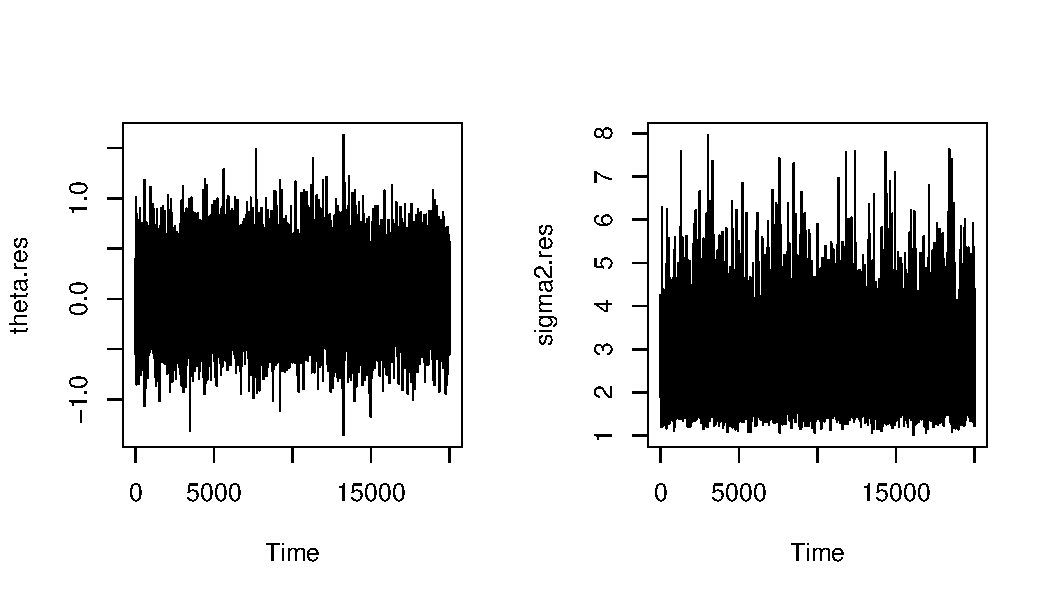
\includegraphics[width=\maxwidth]{figure/unnamed-chunk-7-1} 
\begin{kframe}\begin{alltt}
\hlkwd{acf}\hlstd{(theta.res)}
\hlkwd{acf}\hlstd{(sigma2.res)}
\end{alltt}
\end{kframe}
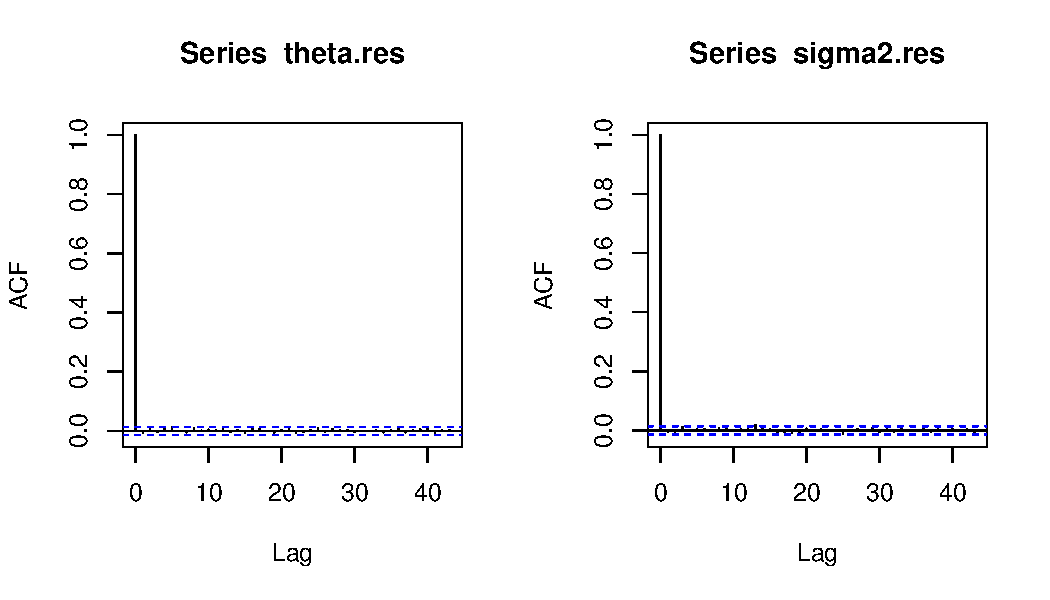
\includegraphics[width=\maxwidth]{figure/unnamed-chunk-7-2} 
\begin{kframe}\begin{alltt}
\hlcom{# Estimaciones puntuales}
\hlkwd{mean}\hlstd{(theta.res)}
\end{alltt}
\begin{verbatim}
## [1] 0.073
\end{verbatim}
\begin{alltt}
\hlkwd{mean}\hlstd{(sigma2.res)}
\end{alltt}
\begin{verbatim}
## [1] 2.5
\end{verbatim}
\begin{alltt}
\hlcom{# Intervalos de credibilidad del 95%}
\hlkwd{quantile}\hlstd{(theta.res,} \hlkwd{c}\hlstd{(}\hlnum{0.025}\hlstd{,}\hlnum{0.975}\hlstd{))}
\end{alltt}
\begin{verbatim}
##  2.5%   98% 
## -0.53  0.67
\end{verbatim}
\begin{alltt}
\hlkwd{quantile}\hlstd{(sigma2.res,} \hlkwd{c}\hlstd{(}\hlnum{0.025}\hlstd{,}\hlnum{0.975}\hlstd{))}
\end{alltt}
\begin{verbatim}
## 2.5%  98% 
##  1.5  4.4
\end{verbatim}
\end{kframe}
\end{knitrout}

Podemos comprobar de las gráficas de los valores simulados que no hay necesidad de descartar los primeros valores obtenidos; de la misma forma, de los correlogramas se puede observar que los valores simulados no incorrelacionados entre ellos, por lo cual podemos calcular las estimaciones directamente usando los 20 mil valores simulados. 

La estimación e intervalo de credibilidad para $\theta$ calculada desde los valores simulados corresponden a 0.073 y (-0.53, 0.67); mientras que para $\sigma^2$, están dadas por 2.5 y (1.5, 4.4). Podemos ver que los resultados obtenidos en los dos enfoques son muy similares.
\end{Eje}

\subsection{Parámetros no informativos}
En esta sección consideramos el tratamiento cuando no tenemos información previa disponible.

Suponga que $\mathbf{Y}=\{Y_1,\ldots,Y_n\}$ corresponde a una muestra de variables aleatorias con distribución $Normal(\theta,\sigma^2)$. Luego, la función de distribución conjunta o verosimilitud está dada por \ref{vero_normal}

\begin{equation*}
p(\mathbf{Y} \mid \theta, \sigma^2)=\frac{1}{(2\pi\sigma^2)^{n/2}}\exp\left\{-\frac{1}{2\sigma^2}\sum_{i=1}^n(y_i-\theta)^2\right\}
\end{equation*}

En primer lugar suponga que los parámetros tienen distribuciones previa independientes y en esta primera etapa se realizará el análisis suponiendo que estas distribuciones son no informativas. Lo anterior implica que la distribución previa conjunta de los parámetros de interés está dada por

\begin{equation}
p(\theta,\sigma^2)=p(\theta)p(\sigma^2)
\end{equation}

Como la distribución previa de $\theta$ es normal, es fácil verificar que ésta empieza a tener las características propias de una distribución no informativa cuando la varianza de la misma se vuelve muy grande, sin importar el valor de la media. Cuando esto sucede, entonces la forma de la distribución previa de $\theta$ se torna plana y es lógico pensar que puede ser acercada mediante una distribución constante, tal que
\begin{equation*}
p(\theta)\propto cte
\end{equation*}

Por otro lado, \citeasnoun{Gelman03} afirma que la distribución Inversa-Gamma, la cual es la distribución previa para el parámetro $\sigma^2$, se vuelve no informativa cuando los hiper-parámetros toman valores muy cercanos a cero. De esta forma haciendo tender $\alpha \longrightarrow 0$ y $\beta \longrightarrow 0$, entonces la distribución previa de $\sigma^2$ se convierte en
\begin{equation*}
p(\sigma^2)\propto \sigma^{-2}
\end{equation*}

la cual coincide con la distribución previa no informativa de Jeffreys discutida en la sección \ref{Normal_Varianza}. Por lo anterior, la distribución previa no informativa conjunta estaría dada por
\begin{equation}\label{previa_noinfo_conjunta}
p(\theta,\sigma^2)\propto \sigma^{-2}
\end{equation}

Bajo este marco de referencia se tiene el siguiente resultado sobre la distribución posterior de $\theta$
\begin{Res}\label{pos_theta_no_informativa}
La distribución posterior del parámetro $\theta$ sigue una distribución $t$ no estandarizado con grado de libertad $n-1$, el parámetro de localización $\bar{Y}$ y el parámetro de escala $\frac{S^2}{n}$, esto es, 
\begin{equation*}
\theta \mid \mathbf{Y}\sim t_{n-1}\left(\bar{y},\frac{S^2}{n}\right).
\end{equation*}

Donde $(n-1)S^2=\sum_{i=1}^n(Y_i-\bar{Y})^2$. Esta distribución también puede expresarse como
\begin{equation*}
\frac{\theta-\bar{y}}{S/\sqrt{n}} \mid \mathbf{Y} \sim t_{n-1}
\end{equation*}

donde $t_{n-1}$ denota la distribución $t$ estandarizado con grado de libertad $n-1$.
\end{Res}

\begin{proof}
En primer lugar nótese que la distribución posterior conjunta de los parámetros de interés es
\begin{align}\label{prop_theta_sigma2}
p(\theta,\sigma^2 \mid \mathbf{Y})& \propto p(\theta,\sigma^2)p(\mathbf{Y} \mid \theta,\sigma^2) \notag \\
& \propto \frac{1}{\sigma^2}\frac{1}{(2\pi\sigma^2)^{n/2}}\exp\left\{-\frac{1}{2\sigma^2}\sum_{i=1}^n(y_i-\theta)^2\right\} \notag\\
& \propto \left(\frac{1}{\sigma^2}\right)^{n/2+1}
\exp\left\{-\frac{1}{2\sigma^2}\left[\sum_{i=1}^n(y_i-\bar{y})^2+n(\bar{y}-\theta)^2\right]\right\} \notag \\
&= \left(\frac{1}{\sigma^2}\right)^{n/2+1}
\exp\left\{-\frac{1}{2\sigma^2}\left[(n-1)S^2+n(\bar{y}-\theta)^2\right]\right\}
\end{align}
Ahora, para hallar la distribución marginal posterior de $\theta$ es necesario integrar la anterior expresión con respecto a $\sigma^2$. Con esto, se tiene que
\begin{align*}
p(\theta \mid \mathbf{Y})&= \int_0^{\infty} p(\theta,\sigma^2 \mid \mathbf{Y}) \ d\sigma^2 \\
&\propto \int_0^{\infty} \left(\frac{1}{\sigma^2}\right)^{n/2+1}
\exp\left\{-\frac{1}{2\sigma^2}\left[(n-1)S^2+n(\bar{y}-\theta)^2\right]\right\} \ d\sigma^2
\end{align*}
Haciendo un cambio de variable tal que
\begin{equation*}
z=\frac{A}{2\sigma^2}, \ \ \ \ \ \ \ \ \ \ \ \text{donde} \ \ \ A=(n-1)S^2+n(\bar{y}-\theta)^2
\end{equation*}
por tanto
\begin{equation*}
d\sigma^2=-\frac{A}{2z^2} \ dz
\end{equation*}
Entonces, volviendo a la integral en cuestión, se tiene que
\begin{align*}
p(\theta \mid \mathbf{Y})& \propto
\left(\frac{1}{A}\right)^{n/2+1}\int_{\infty}^{0} \frac{-A}{2z^2} (2z)^{n/2+1}e^{-z} \ dz \\
&\propto A^{-n/2}\underbrace{\int_{0}^{\infty} z^{n/2-1}e^{-z}\ dz}_{Gamma(n/2)}\\
&\propto A^{-n/2}\\
&= [(n-1)S^2+n(\bar{y}-\theta)^2]^{-n/2}\\
&\propto \left[1+\frac{n(\bar{y}-\theta)^2}{(n-1)S^2}\right]^{-n/2}
=\left[1+\frac{1}{n-1}\left(\frac{\bar{y}-\theta}{S/\sqrt{n}}\right)^2\right]^{-\frac{(n-1)+1}{2}}
\end{align*}
la cual corresponde a la función de densidad de distribución de una variable aleatoria con distribución $t_{n-1}(\bar{y},S^2/n)$.
\end{proof}

\begin{Res}\label{pos_sigma2_no_informativa}
La distribución posterior del parámetro $\sigma^2$ sigue una distribución
\begin{equation*}
\sigma^2 \mid \mathbf{Y} \sim Inversa-Gamma((n-1)/2,(n-1)S^2/2).
\end{equation*}
\end{Res}

\begin{proof}
Utilizando el mismo argumento del anterior resultado, se tiene que
\begin{align*}
p(\sigma^2 \mid \mathbf{Y})&= \int_{-\infty}^{\infty} p(\theta,\sigma^2 \mid \mathbf{Y}) \ d\theta \\
& \propto \int_{-\infty}^{\infty} \left(\frac{1}{\sigma^2}\right)^{n/2+1}
\exp\left\{-\frac{1}{2\sigma^2}\left[(n-1)S^2+n(\bar{y}-\theta)^2\right]\right\} \ d\theta \\
& = \left(\frac{1}{\sigma^2}\right)^{n/2+1} \sqrt{2\pi\sigma^2/n}\exp\left\{-\frac{1}{2\sigma^2}(n-1)S^2\right\}\underbrace{\int_{-\infty}^{\infty} \frac{1}{\sqrt{2\pi\sigma^2/n}} \exp\left\{-\frac{n}{2\sigma^2}(\bar{y}-\theta)^2\right\} \ d\theta}_{\text{vale $1$}} \\
& \propto (\sigma^2)^{-n/2-1/2}\exp\left\{-\frac{1}{2\sigma^2}(n-1)S^2\right\}\\
&= (\sigma^2)^{-\frac{n-1}{2}-1}\exp\left\{-\frac{1}{2\sigma^2}(n-1)S^2\right\}
\end{align*}
la cual corresponde a la función de densidad de la distribución $Inversa-Gamma((n-1)/2,(n-1)S^2/2)$.
\end{proof}

De los resultados \ref{pos_theta_no_informativa} y \ref{pos_sigma2_no_informativa}, podemos ver que cuando no se dispone de información previa, la estimación bayesiana de $\theta$ y $\sigma^2$ están dadas por
\begin{align*}
\hat{\theta}_B&=E(\theta\mid\mathbf{Y})=\bar{Y}\\
\hat{\sigma}^2_B&=E(\sigma^2\mid\mathbf{Y})=\dfrac{(n-1)S^2/2}{(n-1)/2-1}=\dfrac{n-1}{n-3}S^2\approx S^2
\end{align*}
Podemos concluir que la estimación bayesiana de $\theta$ cuando no hay información previa es idéntica a la estimación clásica de $\theta$, mientas que la de $\sigma^2$ es muy similar a la estimación clásica.

En cuanto a la estimación por intervalo, podemos ver que un intervalo de crediblidad de $(1-\alpha)\times 100\%$ está dado por los percentiles $\alpha/2$ y $1-\alpha/2$ de la distribución $t_{n-1}\left(\bar{Y},\dfrac{S^2}{n}\right)$, se puede ver que estos corresponden a $\bar{Y}+t_{n-1,\alpha/2}\dfrac{S}{\sqrt{n}}$ y $\bar{Y}+t_{n-1,1-\alpha/2}\dfrac{S}{\sqrt{n}}$. En conclusión, un intervalo de credibildad para $\theta$ está dado por $\bar{Y}\pm t_{n-1,1-\alpha/2}\dfrac{S}{\sqrt{n}}$, el cual es idéntico al intervalo de confianza para $\theta$ en la estadística clásica.

En cuanto al intervalo de crediblidad para $\sigma^2$, este está dado por los percentiles $\alpha/2$ y $1-\alpha/2$ de la distribución $Inversa-Gamma((n-1)/2,\ (n-1)S^2/2)$. En la estadística clásica, el intervalo de confianza para $\sigma^2$ está dada por \begin{equation*}
IC(\sigma^2)=\left(\dfrac{(n-1)S^2}{\chi^2_{n-1,1-\alpha/2}},\ \dfrac{(n-1)S^2}{\chi^2_{n-1,\alpha/2}}\right)
\end{equation*}

Aunque la forma de estos dos intervalos son muy diferentes, resultan ser idénticos. A continuación mostramos el porqué. Suponga que $a$ es el percentil $\alpha/2$ de la distribución $Inversa-Gamma((n-1)/2,\ (n-1)S^2/2)$, esto es, si $X\sim Inversa-Gamma((n-1)/2,\ (n-1)S^2/2)$, entonces $Pr(X<a)=\alpha/2$. Ahora por propiedades de la distribución $Inversa-Gamma$, se tiene que $\dfrac{X}{(n-1)S^2}\sim Inversa-Gamma(\frac{n-1}{2},\ \frac{1}{2})$. Por la relación entre la distribución $Gamma$ y la distribución $Inversa-Gamma$, tenemos que $\dfrac{(n-1)S^2}{X}\sim Gamma(\frac{n-1}{2},\ 2)$, es decir, $\dfrac{(n-1)S^2}{X}\sim\chi^2_{n-1}$, de donde tenemos que
\begin{align*}
\frac{\alpha}{2}&=Pr(X<a)\\
&=Pr\left(\dfrac{(n-1)S^2}{X}>\dfrac{(n-1)S^2}{a}\right)
\end{align*}

Esto es, $\dfrac{(n-1)S^2}{a}$ es el percentil $1-\alpha/2$ de la distribución $\chi^2_{n-1}$, esto es,  $\dfrac{(n-1)S^2}{a}=\chi^2_{n-1,1-\alpha/2}$, de donde $a=\dfrac{(n-1)S^2}{\chi^2_{n-1,1-\alpha/2}}$, así concluimos que el límite inferior del intervalo de credibildad coincide con el límite inferior del intervalo de confianza. Análogamente se puede ver que también los límites superiores coinciden, y así vemos que el intervalo para $\sigma^2$ coincide en la estadística clásica y la estadística bayesiana sin información previa.

\textbf{\emph{Enfoque alterno para estimar $\theta$ y $\sigma^2$}}

Existe otra forma de obtener las estimaciones para el parámetro $\theta$, recordando la expresión \ref{prop_theta_sigma2}, podemos afirmar que 
\begin{equation*}
\theta \mid \sigma^2, \mathbf{Y} \sim Normal(\bar{y},\sigma^2/n)
\end{equation*}

puesto que 
\begin{align*}
p(\theta \mid \sigma^2,\mathbf{Y})&\propto p(\theta, \sigma^2 \mid\mathbf{Y})\\
&\propto\exp\left\{-\frac{1}{2\sigma^2}\left[(n-1)S^2+n(\bar{y}-\theta)^2\right]\right\}\\
&=\exp\left\{-\frac{n}{2\sigma^2}(\bar{y}-\theta)^2\right\}
\end{align*}

la cual corresponde a la función de densidad de la distribución $Normal(\bar{y},\sigma^2/n)$. De esta forma, usando las distribución $p(\sigma^2\mid\mathbf{Y})$ y $p(\theta\mid\sigma^2,\mathbf{Y})$, podemos implementar el siguiente procedimiento para obtener valores simulados de $\theta$ y $\sigma^2$: 

Si el número de iteraciones se fija como $G$, entonces se procede a:
\begin{enumerate}[(1)]
\item Simular $G$ valores de la distribución de $\sigma^2|\mathbf{Y}$, es decir, de la distribución $Inversa-Gamma((n-1)/2,(n-1)S^2/2)$, estos valores se denotan por $\sigma^2_{(1)},\sigma^2_{(2)},\cdots,\sigma^2_{(G)}$.
\item  Para cada valor de $\sigma^2_{(g)}$, con $g=1,\cdots,G$, simlar un valor de la distribución de $\theta|\sigma^2,\mathbf{Y}$, es decir, de la distribución $N(\bar{y},\sigma^2/n)$, donde $\sigma^2$ se reemplaza por $\sigma^2_{(g)}$. De sta forma, se obtiene los valores $\theta_{(1)},\theta_{(2)},\cdots,\theta_{(G)}$.
\end{enumerate}

Las estimaciones de $\theta$ y $\sigma^2$ se pueden obteer de los valores obtenidos $\theta_{(1)},\theta_{(2)},\cdots,\theta_{(G)}$ y $\sigma^2_{(1)},\sigma^2_{(2)},\cdots,\sigma^2_{(G)}$.

\textbf{\emph{Distribución predictiva}}

La distribución predictiva para una nueva observación $\tilde{Y}$ está dada por 
\begin{align*}
p(\tilde{y}\mid\mathbf{Y})
&=\int\int p(\tilde{y}\mid\theta,\sigma^2) p(\theta,\sigma^2\mid\mathbf{Y})\ d\theta\ d\sigma^2\\
&=\int\int p(\tilde{y}\mid \theta,\sigma^2)p(\theta\mid\sigma^2,\mathbf{Y})p(\sigma^2\mid\mathbf{Y})\ d\theta\ d\sigma^2\\
&=\int\left(\int p(\tilde{y}\mid \theta,\sigma^2)p(\theta\mid\sigma^2,\mathbf{Y})\ d\theta\right)p(\sigma^2\mid\mathbf{Y})\ d\sigma^2\\
\end{align*}

En la integral dentro del paréntesis, el parámetro $\sigma^2$ permanece fijo, por lo cual, dicha integral es la misma a la del resultado \ref{pred_y_theta}, y corresponde a la distribución $N\left(\bar{y},\left(1+\dfrac{1}{n}\right)\sigma^2\right)$. De esta forma, combinando con la distribución posterior de $\sigma^2$, tenemos que
\begin{align*}
&\ \ \ \ p(\tilde{y}\mid\mathbf{Y})\\
&=\int_0^\infty \dfrac{1}{\sqrt{2\pi(1+\frac{1}{n})\sigma^2}}\exp\left\{-\dfrac{1}{2\sigma^2(1+\frac{1}{n})}(\tilde{y}-\bar{y})^2\right\}\dfrac{\left(\frac{(n-1)S^2}{2}\right)^{(n-1)/2}}{\Gamma\left(\frac{n-1}{2}\right)}(\sigma^2)^{-\frac{n-1}{2}-1}\exp\left\{-\dfrac{(n-1)S^2}{2\sigma^2}\right\}\ d\sigma^2
\end{align*}

Después de realizar las manipulaciones algebráicas necesarias, se encuentra que 
\begin{equation}\label{post_y_no_informativa_t_student}
p(\tilde{y}\mid\mathbf{Y})=\dfrac{\Gamma(n/2)}{\Gamma((n-1)/2)}\dfrac{1}{\sqrt{\pi(n-1)}}\left(\left(1+\frac{1}{n}\right)S^2\right)^{-1/2}\left(1+\dfrac{1}{n-1}\dfrac{(\tilde{y}-\bar{y})^2}{\left(1+\frac{1}{n}\right)S^2}\right)^{-n/2}
\end{equation}

la cual corresponde a la distribución $t$ no estandarizado con grado de libertad $n-1$, el parámetro de localización $\bar{y}$ y el parámetro de escala $(1+\frac{1}{n})S^2$. De esta forma, podemos ver que los dos primeros momentos de esta distribución están dados por
\begin{align*}
E(\tilde{Y}\mid\mathbf{Y})&=\bar{y}\\
Var(\tilde{Y}\mid\mathbf{Y})&=\dfrac{n-1}{n-3}\left(1+\frac{1}{n}\right)S^2=\dfrac{(n-1)(n+1)}{n(n-3)}S^2
\end{align*}

Otra manera equivalente de conocer el comportamiento probabilístico de $\tilde{y}$ es por medio de la simulación. Se debe simular en primer lugar valores de $\theta$ y de $\sigma^2$ de la distribución posterior $p(\theta,\ \sigma^2\mid\mathbf{Y})$ usando el muestreador de Gibbs y posteriormente se simula valores de $\tilde{y}$ de la distribución $p(\tilde{y}\mid\theta,\ \sigma^2)$. En la figura \ref{predictiva_y_priori_noninformative} se muestran el histograma de 10 mil valores de $\tilde{Y}$ simulados de esta forma, con 20 datos simulados de la distribución $N(12,3^2)$. En la misma gráfica se observa también la función de densidad de la distribución $t$, podemos ver que los valores de simulados de $\tilde{Y}$ efectivamente coincide con la distribución predictiva de $\tilde{Y}$. Por lo anterior, se puede calcular un predictor de $\tilde{Y}$ como el promedio de los 10 mil valores simulados, y calcular el intervalo de predicción usando los percentiles de estos 10 mil valores.
 
\begin{figure}[!htb]\label{predictiva_y_priori_noninformative}
\centering
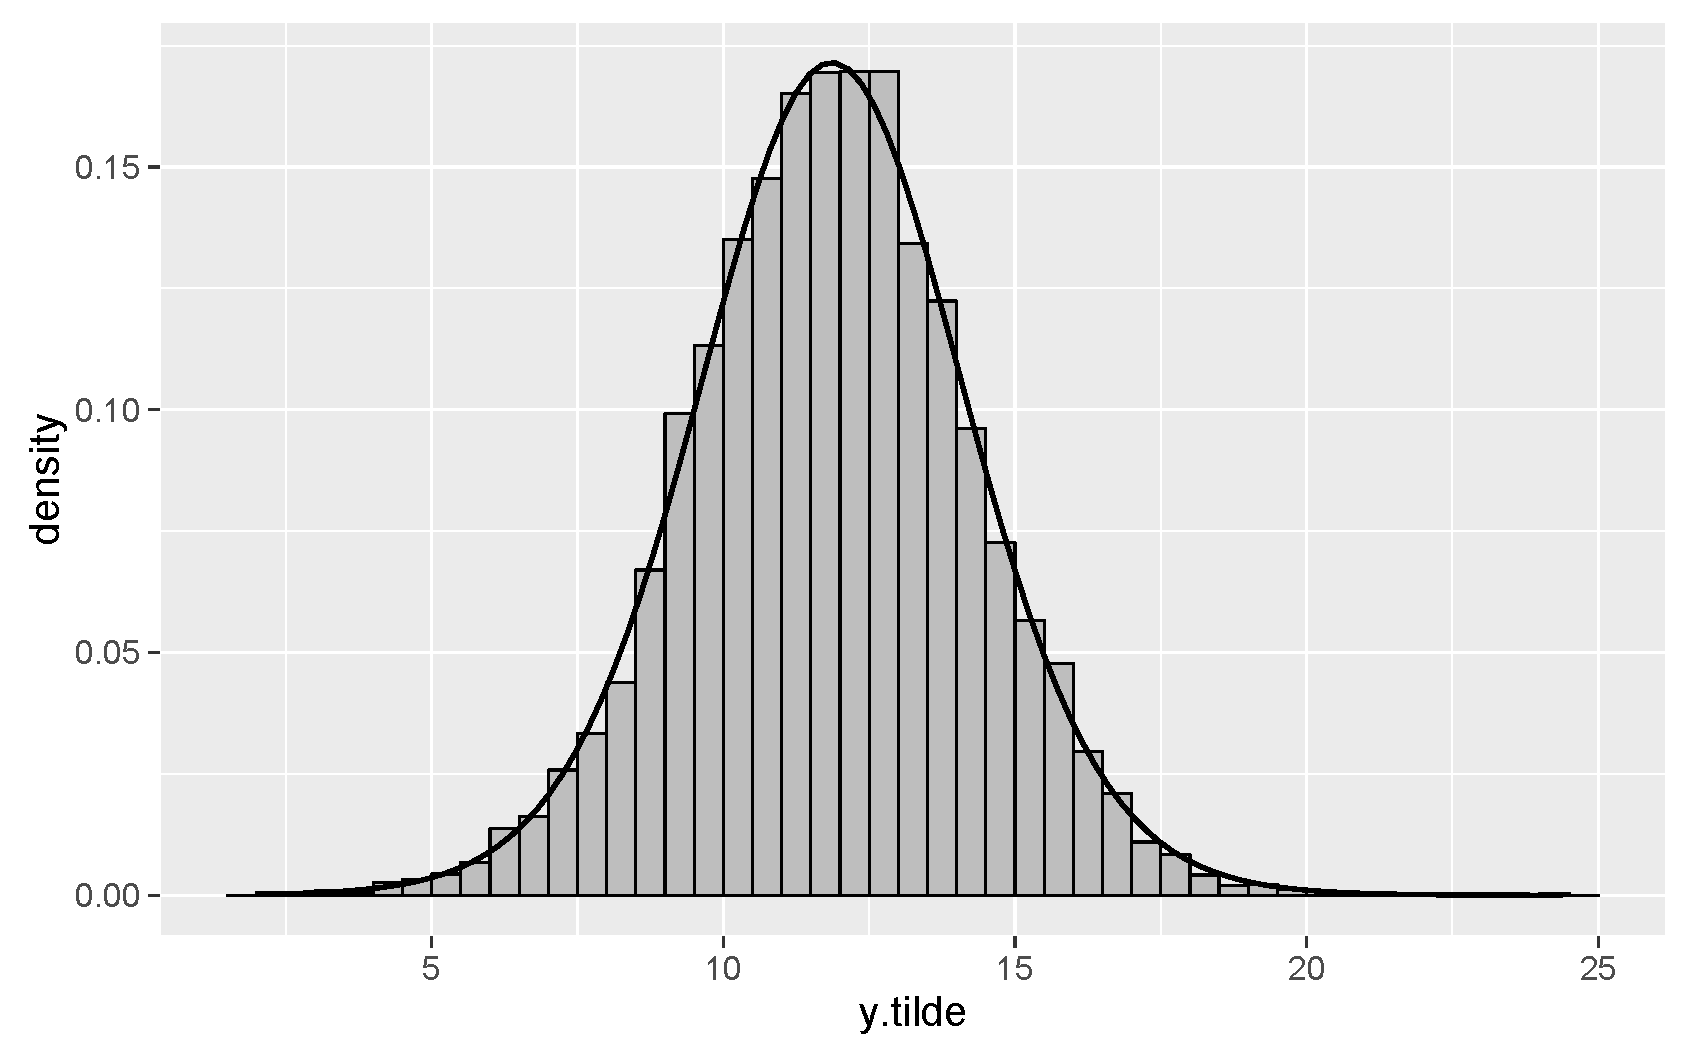
\includegraphics[scale=0.5]{predictiva_y_priori_noninformative.pdf}
\caption{\emph{10 mil valores simulados de $\tilde{Y}$ y la función de densidad de la distribución predictiva de $\tilde{Y}$.}}
\end{figure}

\section{Normal multivariante con media desconocida y varianza conocida}

Cuando la verosimilitud de los datos es una distribución normal multivariante, las técnicas de inferencia no se distancian mucho del caso univariado. Se debe tener en cuenta el manejo matricial de las formas cuadráticas y las propiedades básicas del cálculo de matrices. Los desarrollos y resultados derivados de esta sección redundarán en el análisis de los modelos lineales con el enfoque bayesiano.

Sea $\mathbf{Y}=(Y_1,\ldots,Y_p)'$ un vector aleatorio cuya distribución es normal multivariante dada por

\begin{equation}
p(\mathbf{Y} \mid \btheta,\bSigma)\propto \mid \bSigma \mid ^{-1/2}
\exp\left\{-\frac{1}{2}(\mathbf{y}-\btheta)'\bSigma^{-1}(\mathbf{y}-\btheta)\right\}
  \end{equation}
  
en donde $\btheta=(\theta_1,\ldots,\theta_p)'$ es el vector que contiene la media de cada uno de los componentes del vector y $\bSigma$ es la matriz de varianzas y covarianzas de orden $p\times p$, simétrica y definida positiva. La verosimilitud para una muestra de $n$ vectores aleatorios  independientes e idénticamente distribuidos está dada por
\begin{equation*}\label{Vero_Multi}
  p(\mathbf{Y}_1\ldots,\mathbf{Y}_n \mid \btheta,\bSigma)\propto \mid \bSigma \mid ^{-n/2}
  \exp\left\{-\frac{1}{2}\sum_{i=1}^n(\mathbf{y}_i-\btheta)'\bSigma^{-1}(\mathbf{y}_i-\btheta)\right\}
\end{equation*}
    
Los parámetros que requieren estimación corresponden al vector de medias $\btheta$ y la matriz de varianzas y covarianzas $\bSigma$. Por ahora, se asume que $\bSigma$ es conocida y nos centramos en la estimación del vector de medias $\btheta$. Para la distribución previa, considerando que en general no hay restricción sobre los componentes de $\btheta$, asumimos que $\btheta$ sigue una distribución previa normal multivariante informativa y parametrizada por los hiper parámetros $\bmu$ y $\bGamma$
  \begin{equation*}
p(\btheta \mid \bmu,\bGamma)\propto \mid \bGamma \mid ^{-1/2}
\exp\left\{-\frac{1}{2}(\btheta-\bmu)'\bGamma^{-1}(\btheta-\bmu)\right\}
  \end{equation*}
    
%Nótese que esta distribución se hace no informativa cuando $ \mid \bGamma^{-1} \mid \longrightarrow 0$ sin importar el valor del vector de medias previa $\bmu$.
En el siguiente resultado, encontramos la distribuci\'on posterior del parámetro $\btheta$.
\begin{Res}\label{res_mu_n}
La distribución posterior del vector de parámetros $\bmu$ sigue una distribución normal multivariante
\begin{equation*}
\btheta \mid \mathbf{Y},\bSigma \sim N_p (\bmu_n,\bGamma_n).
\end{equation*}

En donde
\begin{align}\label{mu_nGamma_n}
\bGamma_n &= \left(\bGamma^{-1}+n\bSigma^{-1}\right)^{-1}\\
\bmu_n &= \bGamma_n(\bGamma^{-1}\bmu+n \bSigma^{-1}\bar{\mathbf{y}})
\end{align}
\end{Res}

\begin{proof}
En primer lugar, nótese la siguiente identidad
\begin{equation}
\sum_{i=1}^n(\mathbf{Y}_i-\btheta)'\bSigma^{-1}(\mathbf{Y}_i-\btheta)
=\sum_{i=1}^n(\mathbf{Y}_i-\bar{\mathbf{Y}})'\bSigma^{-1}(\mathbf{Y}_i-\bar{\mathbf{Y}})
+n(\bar{\mathbf{Y}}-\btheta)'\bSigma^{-1}(\bar{\mathbf{Y}}-\btheta)
\end{equation}

que resulta puesto que
\begin{align*}
&\ \ \ \ \sum_{i=1}^n(\mathbf{Y}_i-\btheta)'\bSigma^{-1}(\mathbf{Y}_i-\btheta)\\
&=\sum_{i=1}^n(\mathbf{Y}_i-\bar{\mathbf{Y}}+\bar{\mathbf{Y}}-\btheta)'
\bSigma^{-1}(\mathbf{Y}_i-\bar{\mathbf{Y}}+\bar{\mathbf{Y}}-\btheta)\\
&=\sum_{i=1}^n(\mathbf{Y}_i-\bar{\mathbf{Y}})'\bSigma^{-1}(\mathbf{Y}_i-\bar{\mathbf{Y}})
+\sum_{i=1}^n(\mathbf{Y}_i-\bar{\mathbf{Y}})'\bSigma^{-1}(\bar{\mathbf{Y}}-\btheta)\\
&\hspace{1.5cm}
+(\bar{\mathbf{Y}}-\btheta)'\bSigma^{-1}\sum_{i=1}^n(\mathbf{Y}_i-\bar{\mathbf{Y}})'
+\sum_{i=1}^n(\bar{\mathbf{Y}}-\btheta)'\bSigma^{-1}(\bar{\mathbf{Y}}-\btheta)\\
&=\sum_{i=1}^n(\mathbf{Y}_i-\bar{\mathbf{Y}})'\bSigma^{-1}(\mathbf{Y}_i-\bar{\mathbf{Y}})
+n(\bar{\mathbf{Y}}-\btheta)'\bSigma^{-1}(\bar{\mathbf{Y}}-\btheta)
\end{align*}

Por otro lado, de la definición de distribución previa, se tiene que
\begin{align*}
p(\btheta \mid \mathbf{Y},\bSigma)
&\propto p(\mathbf{Y} \mid \btheta,\bSigma)p(\btheta,\bSigma)\\
&\propto \exp\left\{-\frac{1}{2}\left[\sum_{i=1}^n(\mathbf{y}_i-\btheta)'\bSigma^{-1}(\mathbf{y}_i-\btheta)+(\btheta-\bmu)'\bGamma^{-1}(\btheta-\bmu)\right]\right\}\\
&\propto \exp\left\{-\frac{1}{2}\left[n(\bar{\mathbf{y}}-\btheta)'\bSigma^{-1}(\bar{\mathbf{y}}-\btheta)+(\btheta-\bmu)'\bGamma^{-1}(\btheta-\bmu)\right]\right\}\\
&\propto \exp\left\{-\frac{1}{2}\left[
  -n\bar{\mathbf{y}}'\bSigma^{-1}\btheta-n\btheta'\bSigma^{-1}\bar{\mathbf{y}}+n\btheta'\bSigma^{-1}\btheta+\btheta'\bGamma^{-1}\btheta-\btheta'\bGamma^{-1}\bmu-\bmu'\bGamma^{-1}\btheta\right]\right\}\\
&= \exp\left\{-\frac{1}{2}\left[
  \btheta'(\bGamma^{-1}+n\bSigma^{-1})\btheta-2\btheta'(\bGamma^{-1}\bmu+n\bSigma^{-1}\bar{\mathbf{y}})\right]\right\}\\
&= \exp\left\{-\frac{1}{2}\left[\btheta'\bGamma^{-1}_n\btheta-2\btheta'\bGamma^{-1}_n\bmu_n\right]\right\}\\
&\propto \exp\left\{-\frac{1}{2}\left[\btheta'\bGamma^{-1}_n\btheta-2\btheta'\bGamma^{-1}_n\bmu_n+\bmu_n\bGamma_n^{-1}\bmu_n\right]\right\}\\
&= \exp\left\{-\frac{1}{2}(\btheta-\bmu_n)'\bGamma_n^{-1}(\btheta-\bmu_n)\right\}
  \end{align*}

La cual corresponde al n\'ucleo de una distribuci\'on normal multivariante con el vector de medias $\bmu_n$ y matriz de varianzas $\bGamma_n$.
\end{proof}

Observando los par\'ametros de la distribuci\'on posterior, podemos ver que $\bGamma_n^{-1} = \bGamma^{-1}+(\bSigma/n)^{-1}$. Teniendo en cuenta que la matriz de varianzas y covarianzas es una medida de dispersi\'on de la distribuci\'on alrededor de su media, la inversa de dicha matriz se puede ver como una medida de precisi\'on de qu\'e tanto se concentra la distribuci\'on alrededor de la media. As\'i, podemos ver que la precisi\'on posterior viene siendo la suma entre la precisi\'on previa y la precisi\'on de la estaimaci\'on cl\'asica del parámetro $\btheta$.

En cuanto a la media posterior $\bmu_n$, tenemos que
\begin{align*}
\bmu_n&=\left(\bGamma^{-1}+n\bSigma^{-1}\right)^{-1}
(\bGamma^{-1}\bmu+n \bSigma^{-1}\bar{\mathbf{y}})\\
&=\left(\mathbf{I}+n\bGamma\bSigma^{-1}\right)^{-1}\bmu+\left(\frac{1}{n}\bSigma\bGamma^{-1}+\mathbf{I}\right)^{-1}\bar{\mathbf{y}}\\
&=\bSigma\left(\bSigma+n\bGamma\right)^{-1}\bmu+n\bGamma\left(\bSigma+n\bGamma\right)^{-1}\bar{\mathbf{y}}
\end{align*}

De donde podemos que ver que la media posterior $\bmu_n$ se puede escribir como $\bmu_n=\mathbf{A}_1\bmu+\mathbf{A}_2\bar{\mathbf{y}}$ donde $\mathbf{A}_1+\mathbf{A}_2=\mathbf{I}$. Es claro que en el caso univariado, $\mathbf{A}_1$, $\bmu$, $\mathbf{A}_2$ y $\bar{\mathbf{y}}$ son todos escalares, y $\bmu_n$ es un valor intermedio entre $\bmu$ y $\bar{\mathbf{y}}$, adicionalmente, las matrices $\mathbf{A}_1$ y $\mathbf{A}_2$ son definidas positivas. N\'otese que $\mathbf{A}_1\bmu+\mathbf{A}_2\bar{\mathbf{y}}$ es similar a una combinaci\'on convexa entre los vectores $\bmu$ y $\bar{\mathbf{y}}$, pero los coeficientes son matrices en vez de escalares. 

Para ilustar la relaci\'on de $\bmu_n$ con $\bmu$ y $\bar{\mathbf{y}}$, tomamos el caso de $p=2$, y denotamos $\mathbf{A}=\bSigma\left(\bSigma+n\bGamma\right)^{-1}$. Es claro que $\mathbf{A}$ es una matriz sim\'etrica y definida positiva, lo denotaremos con $\mathbf{A}=\begin{pmatrix}a_{11}&a_{12}\\ a_{12}&a_{22}\end{pmatrix}$, donde $a_{11}>0$ y $a_{22}>0$. De esta forma
\begin{align*}
\bmu_n&=\begin{pmatrix}a_{11}&a_{12}\\ a_{12}&a_{22}\end{pmatrix}\begin{pmatrix}\mu_{1}\\ \mu_{2}\end{pmatrix}+\begin{pmatrix}1-a_{11}&-a_{12}\\ -a_{12}&1-a_{22}\end{pmatrix}\begin{pmatrix}\bar{y}_{1}\\ \bar{y}_{2}\end{pmatrix}\\
&=\begin{pmatrix}a_{11}\mu_1+(1-a_{11})\bar{y}_{1}+a_{12}(\mu_2-\bar{y}_{2})\\a_{22}\mu_2+(1-a_{22})\bar{y}_{2}+a_{12}(\mu_1-\bar{y}_{1})\end{pmatrix}
\end{align*}

Al observar la primera entrada de $\bmu_n$, podemos ver que este se compone de una combinaci\'on convexa entre $\mu_1$ y $\bar{y}_1$ (pues $a_{11}>0$) y una parte que depende de la diferencia $\mu_2-\bar{y}_{2}$; un comportamiento silimar se observa en la segunda entrada de $\bmu_n$. Esta observaci\'on es interesante, pues ilustra que cada componente de la media posterior $\bmu$ no siempre ser\'a un promedio ponderado del componentes corrspondiente de la media previa y la estimaci\'on cl\'asica.

Ilustramos los resultados encontrados suponiendo las dos siguientes situaciones 
\begin{enumerate} 
\item Supong que se quiere estimar el vector de medias $\btheta=(\theta_1,\theta_2)'$ con una matriz de varianzas y covarianzas conocida de $\bSigma=\begin{pmatrix}20&8\\ 8&30\end{pmatrix}$. Para eso tenemos 10 datos que corresponden a vectores bivariadas con $\bar{\mathbf{y}}=(150,230)'$. Como informaci\'on previa, suponga que $\bmu=(100,200)'$ y $\bGamma=\begin{pmatrix}5&3\\ 3&10\end{pmatrix}$. C\'alculos arrojan que $\bGamma_n=\begin{pmatrix}1.42&0.64\\ 0.64&2.31\end{pmatrix}$, $\mathbf{A}=\begin{pmatrix}0.3&-0.026\\ -0.026&0.235\end{pmatrix}$ y $\bmu_n=(136,224)$, podemos ver que en este caso, cada componente de $\bmu_n$ se encuentra entre el componente correspondiente de $\bmu$ y $\bar{\mathbf{y}}$. 
\begin{knitrout}
\definecolor{shadecolor}{rgb}{0.933, 0.933, 0.933}\color{fgcolor}\begin{kframe}
\begin{alltt}
\hlstd{n} \hlkwb{<-} \hlnum{10}
\hlstd{mu} \hlkwb{<-} \hlkwd{matrix}\hlstd{(}\hlkwd{c}\hlstd{(}\hlnum{100}\hlstd{,}\hlnum{200}\hlstd{)); y.bar} \hlkwb{<-} \hlkwd{matrix}\hlstd{(}\hlkwd{c}\hlstd{(}\hlnum{150}\hlstd{,}\hlnum{230}\hlstd{))}
\hlstd{Gamma} \hlkwb{<-} \hlkwd{matrix}\hlstd{(}\hlkwd{c}\hlstd{(}\hlnum{5}\hlstd{,}\hlnum{3}\hlstd{,}\hlnum{3}\hlstd{,}\hlnum{10}\hlstd{),}\hlnum{2}\hlstd{,}\hlnum{2}\hlstd{); Sigma} \hlkwb{<-} \hlkwd{matrix}\hlstd{(}\hlkwd{c}\hlstd{(}\hlnum{20}\hlstd{,}\hlnum{8}\hlstd{,}\hlnum{8}\hlstd{,}\hlnum{30}\hlstd{),}\hlnum{2}\hlstd{,}\hlnum{2}\hlstd{)}
\hlstd{Gamma.n} \hlkwb{<-} \hlkwd{solve}\hlstd{(}\hlkwd{solve}\hlstd{(Gamma)} \hlopt{+} \hlstd{n}\hlopt{*}\hlkwd{solve}\hlstd{(Sigma))}
\hlstd{A} \hlkwb{<-} \hlstd{Sigma} \hlopt \hlkwd{solve}\hlstd{(Sigma} \hlopt{+} \hlstd{n}\hlopt{*}\hlstd{Gamma)}
\hlstd{mu.n} \hlkwb{<-} \hlstd{Gamma.n} \hlopt \hlstd{(}\hlkwd{solve}\hlstd{(Gamma)}\hlopt\hlstd{mu} \hlopt{+} \hlstd{n}\hlopt{*}\hlkwd{solve}\hlstd{(Sigma)}\hlopt\hlstd{y.bar)}
\hlstd{Gamma.n}
\end{alltt}
\begin{verbatim}
##      [,1] [,2]
## [1,] 1.42 0.64
## [2,] 0.64 2.31
\end{verbatim}
\begin{alltt}
\hlstd{A}
\end{alltt}
\begin{verbatim}
##        [,1]   [,2]
## [1,]  0.300 -0.026
## [2,] -0.013  0.235
\end{verbatim}
\begin{alltt}
\hlstd{mu.n}
\end{alltt}
\begin{verbatim}
##      [,1]
## [1,]  136
## [2,]  224
\end{verbatim}
\end{kframe}
\end{knitrout}
\item Tomamos los mismo datos del caso anterior, pero suponga que $\bar{\mathbf{y}}=(150,2300)'$, las matrices $\bGamma_n$ y $\mathbf{A}$ no cambian de valor, pero la media de la distribuci\'on posterior est\'a dada por $\bmu_n=(190,1808)$. Podemos ver que el primer componente de $\bmu_n$ no est\'a entre 100 y 150 que corresponden a las estimaciones previa y cl\'asica, respectivamente, esto se debe a que la diferencia entre $\mu_2$ y $\bar{y}_2$ es muy grande.
\begin{knitrout}
\definecolor{shadecolor}{rgb}{0.933, 0.933, 0.933}\color{fgcolor}\begin{kframe}
\begin{alltt}
\hlstd{y.bar} \hlkwb{<-} \hlkwd{matrix}\hlstd{(}\hlkwd{c}\hlstd{(}\hlnum{150}\hlstd{,}\hlnum{2300}\hlstd{))}
\hlstd{mu.n} \hlkwb{<-} \hlstd{Gamma.n} \hlopt \hlstd{(}\hlkwd{solve}\hlstd{(Gamma)}\hlopt\hlstd{mu} \hlopt{+} \hlstd{n}\hlopt{*}\hlkwd{solve}\hlstd{(Sigma)}\hlopt\hlstd{y.bar)}
\hlstd{mu.n}
\end{alltt}
\begin{verbatim}
##      [,1]
## [1,]  190
## [2,] 1808
\end{verbatim}
\end{kframe}
\end{knitrout}
\end{enumerate}

\textbf{Distribuci\'on previa no informativa}

Al tener en cuenta que la distribución previa del parámetro $\btheta$ es la distribución normal multivariada, y la forma de la función de densidad, se puede afirmar que cuando $|\bGamma^{-1}|$ es muy pequeño, los parámetros previas $\bmu$ y $\bGamma$ pierden peso en los cálculos de $\bmu_n$ y $\bGamma_n$. En este caso se puede ver que
\begin{align*}
\bGamma_n&\approx n^{-1}\bSigma\\
\bmu_n&\approx \bar{\mathbf{y}}
\end{align*}

De donde podemos concluir que la estimación bayesiana será muy cercana a la estimación clásica $\bar{y}$, más aún, el intervalo de credibilidad también será muys similar al intervalo de confianza del enfoque clásico.

\begin{Eje}\label{Eje_Student}
\citeasnoun{Student} introdujo un conjunto de datos clásicos sobre el incremento en horas de sueño producido con 2 medicamentos soporíferos diferentes comparados con grupo control en 10 pacientes. Estos datos se pueden encontrar en \verb'R' con nombre \verb'sleep'. Estos datos se pueden ver como realizaciones de vectores aleatorios con distribución normal bivariada. Supongamos que la matriz de varianzas y covarianzas de la distribución es conocida e igual a $\Sigma=\begin{pmatrix}1&0.6\\ 0.6&2\end{pmatrix}$, y el parámetro de interés es el vector de medias $\btheta=(\theta_1,\theta_2)'$. Para la distribución previa, suponemos que $\bmu=(0,1)'$, es decir que el primer medicamento no tiene ningún efecto soporífero, mientras que el segundo medicamento tiene un efecto promedio de aumentar 1 hora de sueño, también asumimos que $\Gamma=\begin{pmatrix}2&0\\ 0&2\end{pmatrix}$. Los siguientes códigos de \verb'JAGS' ilustra el procedimiento de estimación del parámetro de interés.

\colorbox{black}{\textcolor{white}{\textbf{C\'odigo JAGS}}}
\begin{knitrout}
\definecolor{shadecolor}{rgb}{0.933, 0.933, 0.933}\color{fgcolor}\begin{kframe}
\begin{alltt}
\hlstd{n} \hlkwb{<-} \hlnum{10}
\hlstd{mu}\hlkwb{<-} \hlkwd{as.vector}\hlstd{(}\hlkwd{c}\hlstd{(}\hlnum{0}\hlstd{,}\hlnum{1}\hlstd{)); Gamma} \hlkwb{<-} \hlkwd{matrix}\hlstd{(}\hlkwd{c}\hlstd{(}\hlnum{2}\hlstd{,}\hlnum{0}\hlstd{,}\hlnum{0}\hlstd{,}\hlnum{2}\hlstd{),}\hlnum{2}\hlstd{,}\hlnum{2}\hlstd{)}
\hlstd{Sigma}  \hlkwb{<-} \hlkwd{matrix}\hlstd{(}\hlkwd{c}\hlstd{(}\hlnum{1}\hlstd{,}\hlnum{0.6}\hlstd{,}\hlnum{0.6}\hlstd{,}\hlnum{2}\hlstd{),}\hlnum{2}\hlstd{,}\hlnum{2}\hlstd{); Tau} \hlkwb{<-} \hlkwd{solve}\hlstd{(Sigma)}

\hlstd{NormMult1.model} \hlkwb{<-} \hlkwa{function}\hlstd{()\{}
\hlkwa{for}\hlstd{(i} \hlkwa{in} \hlnum{1} \hlopt{:} \hlstd{n)}
\hlstd{\{}
  \hlstd{y[i,} \hlnum{1}\hlopt{:}\hlnum{2}\hlstd{]} \hlopt{~} \hlkwd{dmnorm}\hlstd{(theta[], Tau[,])}
\hlstd{\}}
\hlstd{theta[}\hlnum{1}\hlopt{:}\hlnum{2}\hlstd{]} \hlopt{~} \hlkwd{dmnorm}\hlstd{(mu[], Gamma[,])}
\hlstd{\}}

\hlstd{y} \hlkwb{<-} \hlkwd{structure}\hlstd{(}\hlkwc{.Data} \hlstd{= sleep[,}\hlnum{1}\hlstd{],} \hlkwc{.Dim}\hlstd{=}\hlkwd{c}\hlstd{(}\hlnum{10}\hlstd{,}\hlnum{2}\hlstd{))}

\hlstd{NormMult1.data} \hlkwb{<-} \hlkwd{list}\hlstd{(}\hlstr{"y"}\hlstd{,}\hlstr{"n"}\hlstd{,}\hlstr{"mu"}\hlstd{,}\hlstr{"Gamma"}\hlstd{,}\hlstr{"Tau"}\hlstd{)}
\hlstd{NormMult1.param} \hlkwb{<-} \hlkwd{c}\hlstd{(}\hlstr{"theta"}\hlstd{)}
\hlstd{NormMult1.inits} \hlkwb{<-} \hlkwa{function}\hlstd{()\{}
\hlkwd{list}\hlstd{(}\hlstr{"theta"}\hlstd{=}\hlkwd{c}\hlstd{(}\hlnum{0}\hlstd{,}\hlnum{0}\hlstd{))}
\hlstd{\}}

\hlstd{NormMult1.fit} \hlkwb{<-} \hlkwd{jags}\hlstd{(}\hlkwc{data}\hlstd{=NormMult1.data,} \hlkwc{inits}\hlstd{=NormMult1.inits, NormMult1.param,}
                      \hlkwc{n.iter}\hlstd{=}\hlnum{10000}\hlstd{,} \hlkwc{n.burnin}\hlstd{=}\hlnum{1000}\hlstd{,} \hlkwc{model.file}\hlstd{=NormMult1.model)}
\end{alltt}
\begin{verbatim}
## Compiling model graph
##    Resolving undeclared variables
##    Allocating nodes
## Graph information:
##    Observed stochastic nodes: 10
##    Unobserved stochastic nodes: 1
##    Total graph size: 25
## 
## Initializing model
\end{verbatim}
\begin{alltt}
\hlkwd{print}\hlstd{(NormMult1.fit)}
\end{alltt}
\begin{verbatim}
## Inference for Bugs model at "/var/folders/c3/jvv2xf7j2zv8xh875zp2hly40000gn/T//RtmpTV9tVM/modelb03e6ebc0360.txt", fit using jags,
##  3 chains, each with 10000 iterations (first 1000 discarded), n.thin = 9
##  n.sims = 3000 iterations saved
##          mu.vect sd.vect   2.5%   25%   50%   75%  98% Rhat n.eff
## theta[1]    0.54    0.28  0.016  0.34  0.53  0.73  1.1    1   940
## theta[2]    1.90    0.38  1.157  1.65  1.91  2.15  2.6    1  3000
## deviance   82.64    2.30 80.164 80.91 82.04 83.71 88.8    1  3000
## 
## For each parameter, n.eff is a crude measure of effective sample size,
## and Rhat is the potential scale reduction factor (at convergence, Rhat=1).
## 
## DIC info (using the rule, pD = var(deviance)/2)
## pD = 2.6 and DIC = 85.3
## DIC is an estimate of expected predictive error (lower deviance is better).
\end{verbatim}
\end{kframe}
\end{knitrout}
De donde podemos que la estimación bayesiana para el aumento de sueño es de 0.54 y 1.90 para los dos medicamentos, respectivament; mientras que los intervalos de crediblidad del 95\% corresponden a (0.016, 1.1) y (1.157, 2.6).

A continuación, mostramos los códigos de \verb'R' para llevar a cabo los mismos cálculos y también realizmos otros analisis interesantes

\colorbox{black}{\textcolor{white}{\textbf{C\'odigo R}}}
\begin{knitrout}
\definecolor{shadecolor}{rgb}{0.933, 0.933, 0.933}\color{fgcolor}\begin{kframe}
\begin{alltt}
\hlstd{n} \hlkwb{<-} \hlnum{10}
\hlstd{Sigma}  \hlkwb{<-} \hlkwd{matrix}\hlstd{(}\hlkwd{c}\hlstd{(}\hlnum{1}\hlstd{,}\hlnum{0.6}\hlstd{,}\hlnum{0.6}\hlstd{,}\hlnum{2}\hlstd{),}\hlnum{2}\hlstd{,}\hlnum{2}\hlstd{)}
\hlstd{mu}\hlkwb{<-} \hlkwd{as.vector}\hlstd{(}\hlkwd{c}\hlstd{(}\hlnum{0}\hlstd{,}\hlnum{1}\hlstd{))}
\hlstd{Gamma} \hlkwb{<-} \hlkwd{matrix}\hlstd{(}\hlkwd{c}\hlstd{(}\hlnum{2}\hlstd{,}\hlnum{0}\hlstd{,}\hlnum{0}\hlstd{,}\hlnum{2}\hlstd{),}\hlnum{2}\hlstd{,}\hlnum{2}\hlstd{)}
\hlstd{y.bar} \hlkwb{<-} \hlkwd{matrix}\hlstd{(}\hlkwd{c}\hlstd{(} \hlkwd{mean}\hlstd{(sleep[sleep}\hlopt{$}\hlstd{group}\hlopt{==}\hlnum{1}\hlstd{,}\hlnum{1}\hlstd{]),} \hlkwd{mean}\hlstd{(sleep[sleep}\hlopt{$}\hlstd{group}\hlopt{==}\hlnum{2}\hlstd{,}\hlnum{1}\hlstd{])))}
\hlstd{Gamma.n} \hlkwb{<-} \hlkwd{solve}\hlstd{(}\hlkwd{solve}\hlstd{(Gamma)} \hlopt{+} \hlstd{n}\hlopt{*}\hlkwd{solve}\hlstd{(Sigma))}
\hlstd{mu.n} \hlkwb{<-} \hlstd{Gamma.n}\hlopt\hlstd{(}\hlkwd{solve}\hlstd{(Gamma)}\hlopt\hlstd{mu} \hlopt{+} \hlstd{n}\hlopt{*}\hlkwd{solve}\hlstd{(Sigma)}\hlopt\hlstd{y.bar)}
\hlstd{Gamma.n}
\end{alltt}
\begin{verbatim}
##       [,1]  [,2]
## [1,] 0.094 0.052
## [2,] 0.052 0.180
\end{verbatim}
\begin{alltt}
\hlstd{mu.n}
\end{alltt}
\begin{verbatim}
##      [,1]
## [1,] 0.68
## [2,] 2.19
\end{verbatim}
\end{kframe}
\end{knitrout}
De los resultados arrojados, vemos que la distribución posterior del parámetro está dada por
\begin{equation*}
\begin{pmatrix}
\theta_1\\
\theta_2
\end{pmatrix}
\sim N_2\left(\begin{pmatrix}
0.68\\
2.19
\end{pmatrix},\begin{pmatrix}
0.094&0.052\\
0.052&0.180
\end{pmatrix}\right)
\end{equation*}

De esta forma, la estimación bayesiana obtenida para los efectos promedios corresponde a 0.68 horas y 2.19 horas, respectivamente, que son similares a los obtenidos por \verb'JAGS'. En cuanto a los intervalos de credibilidad del 95\%, estas son dados por los percentiles 2.5\% y 97.5\% de las dos distribuciones posteriores marginales de $\theta_1$ y $\theta_2$. Estos intervalos se pueden obtener así:
\begin{knitrout}
\definecolor{shadecolor}{rgb}{0.933, 0.933, 0.933}\color{fgcolor}\begin{kframe}
\begin{alltt}
\hlkwd{qnorm}\hlstd{(}\hlkwd{c}\hlstd{(}\hlnum{0.025}\hlstd{,}\hlnum{0.975}\hlstd{),mu.n[}\hlnum{1}\hlstd{],}\hlkwd{sqrt}\hlstd{(Gamma.n[}\hlnum{1}\hlstd{,}\hlnum{1}\hlstd{]))}
\end{alltt}
\begin{verbatim}
## [1] 0.08 1.28
\end{verbatim}
\begin{alltt}
\hlkwd{qnorm}\hlstd{(}\hlkwd{c}\hlstd{(}\hlnum{0.025}\hlstd{,}\hlnum{0.975}\hlstd{),mu.n[}\hlnum{2}\hlstd{],}\hlkwd{sqrt}\hlstd{(Gamma.n[}\hlnum{2}\hlstd{,}\hlnum{2}\hlstd{]))}
\end{alltt}
\begin{verbatim}
## [1] 1.4 3.0
\end{verbatim}
\end{kframe}
\end{knitrout}
Ahora, suponga que el objetivo es comparar los medicmantos para concluir si el segundo medicamento es más efectivo que el primero, podemos encontrar la distribución posterior de la diferencia $\theta_2-\theta_1$, utilizando propiedades de la distribución normal multivariante, podemos encontrar la distribución posterior de $\theta_2-\theta_1$, calcular un intervalo de credibildiad para $\theta_2-\theta_1$ e indagar cuál es la probabilidad de que $\theta_2$ sea mayor a $\theta_1$. Estos cálculos se pueden llevar a cabo de la siguiente forma
\begin{knitrout}
\definecolor{shadecolor}{rgb}{0.933, 0.933, 0.933}\color{fgcolor}\begin{kframe}
\begin{alltt}
\hlstd{vec} \hlkwb{<-} \hlkwd{matrix}\hlstd{(}\hlkwd{c}\hlstd{(}\hlopt{-}\hlnum{1}\hlstd{,}\hlnum{1}\hlstd{),}\hlnum{1}\hlstd{,}\hlnum{2}\hlstd{)}
\hlstd{media} \hlkwb{<-} \hlstd{vec} \hlopt \hlstd{mu.n; varianza} \hlkwb{<-} \hlstd{vec} \hlopt \hlstd{Gamma.n} \hlopt \hlkwd{t}\hlstd{(vec)}
\hlstd{media}
\end{alltt}
\begin{verbatim}
##      [,1]
## [1,]  1.5
\end{verbatim}
\begin{alltt}
\hlstd{varianza}
\end{alltt}
\begin{verbatim}
##      [,1]
## [1,] 0.17
\end{verbatim}
\begin{alltt}
\hlkwd{qnorm}\hlstd{(}\hlkwd{c}\hlstd{(}\hlnum{0.025}\hlstd{,}\hlnum{0.975}\hlstd{),media,}\hlkwd{sqrt}\hlstd{(varianza))}
\end{alltt}
\begin{verbatim}
## [1] 0.7 2.3
\end{verbatim}
\begin{alltt}
\hlnum{1}\hlopt{-}\hlkwd{pnorm}\hlstd{(}\hlnum{0}\hlstd{, media,} \hlkwd{sqrt}\hlstd{(varianza))}
\end{alltt}
\begin{verbatim}
## [1] 1
\end{verbatim}
\end{kframe}
\end{knitrout}
Observando los anteriores resultados, vemos que el intervalo de credibildad para $\theta_2-\theta_1$ está dado por $(0.7, 2.3)$, el cual no contiene el valor 0, indicando que el segundo medicamento tiene un efecto mayor que el segundo. Adicionalmente vemos que con probabilidad 1, el segundo medicamento tiene efecto mayor al primero. Finalmente, podemos visulizar la distribución posterior con los siguientes comandos:
\begin{knitrout}
\definecolor{shadecolor}{rgb}{0.933, 0.933, 0.933}\color{fgcolor}\begin{kframe}
\begin{alltt}
\hlkwd{curve}\hlstd{(}\hlkwd{dnorm}\hlstd{(x, media,} \hlkwd{sqrt}\hlstd{(varianza)),} \hlopt{-}\hlnum{2}\hlstd{,} \hlnum{6}\hlstd{,} \hlkwc{main}\hlstd{=}\hlkwd{expression}
      \hlstd{(}\hlkwd{paste}\hlstd{(}\hlstr{"Distribución posterior de "}\hlstd{, theta[}\hlnum{1}\hlstd{]} \hlopt{-} \hlstd{theta[}\hlnum{2}\hlstd{])),}\hlkwc{ylab}\hlstd{=}\hlstr{""}\hlstd{)}
\hlkwd{abline}\hlstd{(}\hlkwc{v}\hlstd{=}\hlnum{0}\hlstd{)}
\end{alltt}
\end{kframe}
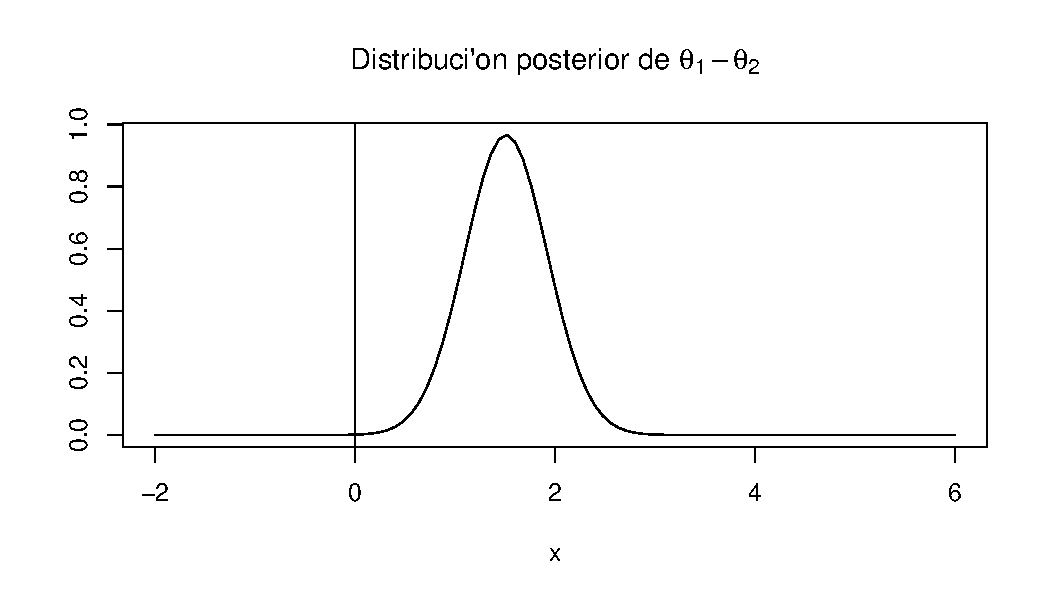
\includegraphics[width=\maxwidth]{figure/unnamed-chunk-14-1} 

\end{knitrout}

De esta forma, podemos concluir que el segundo medicamento tiene un desempeño superior al primero.

Finalmente, ilustramos los resultados obtenidos al usar una distribución previa no informativa, para eso, usaremos $\bGamma=\begin{pmatrix}100&0\\ 0&100\end{pmatrix}$, con $|\bGamma^{-1}|=0.0001$, representando una distribución previa no informativa. Los resultados de estimación arroja la siguiente distribución posterior para el vectro de parámetros 
\begin{equation*}
\begin{pmatrix}
\theta_1\\
\theta_2
\end{pmatrix}
\sim N_2\left(\begin{pmatrix}
0.75\\
2.33
\end{pmatrix},\begin{pmatrix}
0.10&0.06\\
0.06&0.20
\end{pmatrix}\right)
\end{equation*}

Los intervalos de credibilidad del 95\% para los parámetros $\theta_1$ y $\theta_2$ están dados por $(0.129, 1.368)$ y $(1.451, 3.202)$, respectivamente. Observamos que estos intervalos de credibilidad son muy similares a los intervalos de confianza del 95\% del enfoque clásico\footnote{Estos intervalos de confianza fueron calculados con la expresión $\bar{y}\pm z_{1-\alpha/2}\frac{\sigma}{\sqrt{n}}$} dados por $(0.130, 1.370)$ y $(1.453, 3.207)$. En cuanto a la comparación entre los dos medicamentos, lo dejamos como ejercicio para los lectores.
\end{Eje}

Ahora, usando propiedades de la distribución normal multivariante, tenemos los dos siguientes resultados que nos permiten realizar inferencia acerca de un subvector de $\btheta$.
\begin{Res}
La distribución posterior marginal de un subconjunto de parámetros, digamos $\btheta^{(1)}$ es también normal multivariante con media igual a la del subvector de medias apropiado, $\bmu_n^{(1)}$ y similar matriz de varianzas $\bGamma_n^{(11)}$.
\end{Res}
  
\begin{Res}
  La distribución posterior condicional de un subconjunto de parámetros, digamos $\btheta^{(1)}$, dado $\btheta^{(2)}$ es también normal multivariante dada por
  \begin{equation*}
  \btheta^{(1)} \mid \btheta^{(2)} \sim N_p \left(\bmu_n^{(1)}+\bGamma_n^{(12)}\left(\bGamma_n^{(22)}\right)^{-1}
  \left(\theta^{(2)}-\mu_n^{(2)}\right),\bGamma_n^{(1 \mid 2)}\right).
  \end{equation*}
  En donde
  \begin{align}
  \bGamma_n^{(1 \mid 2)}&= \bGamma_n^{(11)}-\bGamma_n^{(12)}\left(\bGamma_n^{(22)}\right)^{-1}\bGamma_n^{(21)}
  \end{align}

$\bmu^{(1)}$ y $\bmu^{(2)}$ corresponden al vector de medias y $\bGamma_n^{(11)}$, $\bGamma_n^{(22)}$ denotan la matriz de varianzas y covarianzas de $\btheta^{(1)}$ y $\btheta^{(2)}$, respectivamente. $\bGamma_n^{(12)}$ es la matriz de covarianzas entre $\btheta^{(1)}$ y $\btheta^{(2)}$, $\bGamma_n^{(21)}$ es la matriz de covarianzas entre $\btheta^{(2)}$ y $\btheta^{(1)}$. 
\end{Res}
  
La prueba de los dos resultados anteriores se sigue inmediatamente de las propiedades de la distribución normal multivariante.

\section{Normal multivariante con media y varianza desconocida}
  
Al igual que en la distribución normal univariada, cuando se desconoce tanto el vector de medias como la matriz de varianzas y covarianzas de la distribución, es necesario plantear diversos enfoques y situarse en el más conveniente.\footnote{Nótese que en términos de parámetros, existen $p$ parámetros correspondientes al vector de medias $\btheta$ y $\binom{p}{2}=\dfrac{p(p+1)}{2}$ parámetros correspondientes a la matriz de varianzas $\bSigma$. Pensando en la gran cantidad de parámetros que se deben modelar, es necesario tener en cuenta que el número de datos en la muestra aleatoria sea lo suficientemente grande.} Suponiendo que el número de observaciones en la muestra aleatoria sea suficiente, existe otra situación que se debe surtir y es la asignación de las distribuciones previas para $\btheta$ y $\bSigma$. En estos términos, es posible
  
\begin{itemize}
\item Suponer que la distribución previa $p(\btheta)$ es independiente de la distribución previa $p(\bSigma)$ y que ambas distribuciones son informativas. Luego, utilizar un análisis de simulación condicional conjunta para extraer muestras provenientes de las respectivas distribuciones posterior.
\item Suponer que la distribución previa para $\btheta$ depende de $\bSigma$ y escribirla como $p(\btheta \mid \bSigma)$, mientras que la distribución previa de $\bSigma$ no depende de $\btheta$ y se puede escribir como $p(\bSigma)$. El análisis posterior de este enfoque encuentra la distribución posterior de $\bSigma \mid \mathbf{Y}$ y con esta se encuentra la distribución posterior de $\btheta \mid \bSigma,\mathbf{Y}$.
\item Suponer que la distribución previa para $\btheta$ y $\bSigma)$ es una distribución no informativas.
\end{itemize}
  
\subsection{Parámetros independientes con distribuciones previas informativas}

En este enfoque se supone que las distribuciones previas para los parámetros de interés son independientes e informativas. La función de verosimilitud está dada en la expresión $\ref{Vero_Multi}$. Hacemos siguiente observación para lograr que las resultantes distribuciones posterior sean conjugadas. 
\begin{align*}
\sum_{i=1}^n(\mathbf{Y}_i-\theta)'\bSigma^{-1}(\mathbf{Y}_i-\theta)&=traza \left(\sum_{i=1}^n(\mathbf{Y}_i-\theta)'\bSigma^{-1}(\mathbf{Y}_i-\theta)\right)\\
&= \sum_{i=1}^ntraza\left((\mathbf{Y}_i-\theta)'\bSigma^{-1}(\mathbf{Y}_i-\theta)\right)\\
&= \sum_{i=1}^ntraza\left(\bSigma^{-1}(\mathbf{Y}_i-\theta)(\mathbf{Y}_i-\theta)'\right)\\
&= traza\left(\bSigma^{-1}\sum_{i=1}^n(\mathbf{Y}_i-\theta)(\mathbf{Y}_i-\theta)'\right)\\
&= traza\left(\bSigma^{-1}\mathbf{S}_{\btheta}\right)
\end{align*}

Donde $\mathbf{S}_{\btheta}=\sum_{i=1}^n(\mathbf{Y}_i-\btheta)(\mathbf{Y}_i-\btheta)'$. En cuanto a la asignación de las distribuciones previas, para el vector de medias $\btheta$ es posible usar la distribución normal, esto es,
\begin{equation*}
\btheta \sim Normal_p(\bmu,\bGamma)
\end{equation*}

Por otro lado, la distribución para la matriz de varianzas $\bSigma$ es
\begin{equation*}
\bSigma \sim Inversa-Wishart(\bLambda,v)
\end{equation*}

donde $v$ denota el grado de libertad y $\bLambda$ la matriz de escala. De esta forma, la función de densidad estádada por
\begin{equation*}
p(\bSigma)\propto |\bSigma|^{-\frac{v+p+1}{2}}\exp\left\{-\frac{1}{2}traza(\bLambda\bSigma^{-1})\right\}
\end{equation*}

Asumiendo independencia previa, la distribución previa conjunta resulta estar dada por
\begin{align}
p(\btheta,\bSigma)&=p(\btheta)p(\bSigma)\notag\\
&\propto \mid \bSigma \mid ^{-(v+p+1)/2}\notag\\
&\times
\exp\left\{ -\frac{1}{2}\left[traza(\bLambda\bSigma^{-1})+
(\btheta-\bmu)'\bGamma^{-1}(\btheta-\bmu)\right]\right\}
\end{align}


Una vez que se conoce la forma estructural de la distribución previa conjunta, es posible establecer la distribución posterior conjunta puesto que la verosimilitud de los datos, $p(\mathbf{Y} \mid \btheta,\bSigma)$, está dada por la expresión (3.3.1), entonces y acudiendo a la simetría de las matrices $\bLambda$, $\bSigma$ y $\mathbf{S}_{\btheta}$, se tiene que
\begin{align}
p(\btheta,\bSigma \mid \mathbf{Y})&=p(\btheta,\bSigma)p(\mathbf{Y} \mid \btheta,\bSigma)\notag\\
&\propto \mid \bSigma \mid ^{-(v+n+p+1)/2}\notag\\
&\times
\exp\left\{ -\frac{1}{2}\left[traza(\bLambda\bSigma^{-1}+\bSigma^{-1}\mathbf{S}_{\btheta})+
                                (\btheta-\bmu)'\bGamma^{-1}(\btheta-\bmu)\right]\right\}\notag\\
                              &\propto \mid \bSigma \mid ^{-(v+n+p+1)/2}\notag\\
                              &\times
                              \exp\left\{ -\frac{1}{2}\left[traza(\bSigma^{-1}(\bLambda+\mathbf{S}_{\btheta}))+
                              (\btheta-\bmu)'\bGamma^{-1}(\btheta-\bmu)\right]\right\}
\end{align}

Dado que la distribución posterior conjunta no tiene una forma estructural conocida, no es posible utilizar el método de integración analítica. Sin embargo, es posible obtener las distribuciones condicionales de cada uno de los parámetros suponiendo fijos los restantes y teniendo en cuenta que
\begin{align*}
p(\btheta \mid \bSigma,\mathbf{Y})\propto p(\btheta,\underbrace{\bSigma}_{fijo} \mid \mathbf{Y})
\ \ \ \ \ \ \ \ \ \text{y} \ \ \ \ \ \ \ \ \ \
p(\bSigma \mid \btheta,\mathbf{Y})\propto p(\underbrace{\btheta}_{fijo},\bSigma \mid \mathbf{Y})
\end{align*}

\begin{Res}
La distribución posterior de la matriz de parámetros $\bSigma$ condicional a $\btheta,\mathbf{Y}$ es
\begin{equation*}\label{Pos_Cond_bSigma}
\bSigma \mid \btheta,\mathbf{Y} \sim Inversa-Wishart_{v+n}(\bLambda+\mathbf{S}_{\btheta})
\end{equation*}
\end{Res}

\begin{proof}
La prueba es inmediata notando que
\begin{align*}
\bSigma \mid \btheta,\mathbf{Y}&\propto\mid \bSigma \mid ^{-(v+n+p+1)/2}\notag\\
&\times\exp\left\{ -\frac{1}{2}\left[traza(\bSigma^{-1}(\bLambda+\mathbf{S}_{\btheta}))+(\btheta-\bmu)'\bGamma^{-1}(\btheta-\bmu)\right]\right\}
\end{align*}

Por lo tanto, factorizando convenientemente, se encuentra una expresión idéntica a la función de distribución de una variable aleatoria con distribución $Inversa-Wishart_{v+n}(\bLambda+\mathbf{S}_{\btheta})$.
\end{proof}
                          
\begin{Res}
La distribución posterior del vector de parámetros $\btheta$ condicional a $\bSigma,\mathbf{Y}$ es
\begin{equation}\label{Pos_Cond_btheta}
\btheta \mid  \bSigma,\mathbf{Y} \sim Normal_p(\bmu_n,\bGamma_n)
\end{equation}
donde $\bmu_n$ y $\bGamma_n$ están dadas por las expresiones (3.2.3) y (3.2.4), respectivamente.
\end{Res}
                              
\begin{proof}
Utilizando el resultado (B.3.5), se tiene que la verosimilitud para los datos observados también se puede escribir como
\begin{align*}
p(\mathbf{Y} \mid \btheta,\bSigma)
&\propto \mid \bSigma \mid ^{-n/2}\exp\left\{-\frac{1}{2}\sum_{i=1}^n(\mathbf{Y}_i-\btheta)'\bSigma^{-1}(\mathbf{Y}_i-\btheta)\right\}
\end{align*}

Por lo tanto, reemplazando la verosimilitud en (3.3.3), se tiene que la distribución posterior conjunta también se puede escribir como
\begin{align*}
p(\btheta,\bSigma \mid \mathbf{Y})
&\propto \mid \bSigma \mid ^{-(v+n+p+1)/2}\notag\\
&\times
\exp\left\{ -\frac{1}{2}\left[\sum_{i=1}^n(\mathbf{Y}_i-\btheta)'\bSigma^{-1}(\mathbf{Y}_i-\btheta)+(\btheta-\bmu)'\bGamma^{-1}(\btheta-\bmu)\right]\right\}
\end{align*}

Y fijando la matriz de parámetros $\bSigma$, se encuentra que la distribución posterior de $\btheta$ condicional a $\bSigma,\mathbf{Y}$ es tal que
\begin{align*}
p(\btheta \mid \bSigma,\mathbf{Y})
\propto
\exp\left\{ -\frac{1}{2}\left[\sum_{i=1}^n
                               (\mathbf{Y}_i-\btheta)'\bSigma^{-1}(\mathbf{Y}_i-\btheta)
                               +(\btheta-\bmu)'\bGamma^{-1}(\btheta-\bmu)\right]\right\}
\end{align*}

La anterior expresión tiene la misma forma estructural que la expresión principal en la demostración del resultado 3.2.1. Luego, siguiendo el mismo razonamiento se llega fácilmente a la prueba.
\end{proof}

Una vez encontradas las distribuciones posteriores condicionales de $\btheta$ y $\bSigma$, se puede obtener la estimación de estos parámetros vía el muestreador de Gibbs, que en este caso se resume en los siguientes pasos:
\begin{enumerate}[(1)]
\item Fijar un valor inicial para $\btheta$, lo denotamos por $\btheta_{(1)}$
\item Simular un valor de la distribución de $\bSigma|\btheta,\mathbf{Y}$ en \ref{Pos_Cond_bSigma} donde el parámetro $\mathbf{S_\mathbf{\btheta}}$ que depende de $\btheta$, debe ser reemplazado por $\btheta_{(1)}$ del paso anterior. Este valor simulado se denotará por $\bSigma_{(1)}$
\item  Simlar un valor de la distribución de $\btheta|\bSigma,\mathbf{Y}$ en \ref{Pos_Cond_btheta} donde en $\mathbf{mu}_n$ y $\bGamma_n$ se debe reemplazar $\bSigma$ por $\bSigma$. Este valor simulado se denota por $\btheta$.
\item Se repite los pasos (2) y (3) hasta completar un número de iteraciones suficientes para alcanzar la convergencia en ambos parámetros
\end{enumerate}
Una vez tengamos los valores muestreados, se debe garantizar la convergencia y la correlación nula entre estos valores, con el fin de calcular las estimaciones. En el siguiente ejemplo ilustramos la implementación de este muestreador de Gibbs en \verb'JAGS' y \verb'R'.

\begin{Eje}\label{Eje_Student_2}
Retomamos los datos del efecto de dos medicamentos soporíferos introducidos por \citeasnoun{Student} que fueron estudiados en el ejemplo \ref{Eje_Student} asumiendo que la matriz de varianzas y covarianzas es conocida. El vector de medias muestrales de estos datos están dados por $\bar{y}=(0.75, 2.33)'$, y la matriz de varianzas y covarianzas muestrales está dada por $\mathbf{S}=\begin{pmatrix}3.20&2.85\\2.85&4.01\end{pmatrix}$. 

Ahora supongamos que tanto el vector de medias como la matriz de varianzas y covarianzas y desconocidos. Para el vectro de medias, asumimos la distribución previa del ejemplo \ref{Eje_Student}, es decir, $\bmu=(0,1)'$ y $\bGamma=\begin{pmatrix}2&0\\0&2\end{pmatrix}$. Para la matriz de varianzas y covarianzas asumimos la distribución inversa Wishart con matriz de escala igual a $\bLambda=\begin{pmatrix}20&8\\8&20\end{pmatrix}$ y grado de libertad $v=10$, de esta forma, la estimación previa de $\bSigma$ viene dada por $\frac{1}{v-2-1}\bLambda=\begin{pmatrix}2.86&1.14\\ 1.14&2.86\end{pmatrix}$. 

Ilustramos los códigos de \verb'JAGS' a continuación.

\colorbox{black}{\textcolor{white}{\textbf{C\'odigo JAGS}}}
\begin{knitrout}
\definecolor{shadecolor}{rgb}{0.933, 0.933, 0.933}\color{fgcolor}\begin{kframe}
\begin{alltt}
\hlstd{n} \hlkwb{<-} \hlnum{10}
\hlstd{mu}\hlkwb{<-} \hlkwd{as.vector}\hlstd{(}\hlkwd{c}\hlstd{(}\hlnum{0}\hlstd{,}\hlnum{1}\hlstd{)); Gamma} \hlkwb{<-} \hlkwd{matrix}\hlstd{(}\hlkwd{c}\hlstd{(}\hlnum{2}\hlstd{,}\hlnum{0}\hlstd{,}\hlnum{0}\hlstd{,}\hlnum{2}\hlstd{),}\hlnum{2}\hlstd{,}\hlnum{2}\hlstd{)}
\hlstd{v} \hlkwb{<-} \hlnum{10}\hlstd{; Lambda} \hlkwb{<-} \hlkwd{matrix}\hlstd{(}\hlkwd{c}\hlstd{(}\hlnum{20}\hlstd{,}\hlnum{8}\hlstd{,}\hlnum{8}\hlstd{,}\hlnum{20}\hlstd{),}\hlnum{2}\hlstd{,}\hlnum{2}\hlstd{)}

\hlstd{NormMult2.model} \hlkwb{<-} \hlkwa{function}\hlstd{()\{}
\hlkwa{for}\hlstd{(i} \hlkwa{in} \hlnum{1} \hlopt{:} \hlstd{n)}
\hlstd{\{}
  \hlstd{y[i,} \hlnum{1}\hlopt{:}\hlnum{2}\hlstd{]} \hlopt{~} \hlkwd{dmnorm}\hlstd{(theta[], Tau[,])}
\hlstd{\}}
\hlstd{theta[}\hlnum{1}\hlopt{:}\hlnum{2}\hlstd{]} \hlopt{~} \hlkwd{dmnorm}\hlstd{(mu[], Gamma[,])}
\hlstd{Tau[}\hlnum{1}\hlopt{:}\hlnum{2}\hlstd{,}\hlnum{1}\hlopt{:}\hlnum{2}\hlstd{]} \hlopt{~} \hlkwd{dwish}\hlstd{(Lambda[,] , v)}
\hlstd{Sigma[}\hlnum{1}\hlopt{:}\hlnum{2}\hlstd{,}\hlnum{1}\hlopt{:}\hlnum{2}\hlstd{]} \hlkwb{<-} \hlkwd{inverse}\hlstd{(Tau[,])}
\hlstd{\}}

\hlstd{y} \hlkwb{<-} \hlkwd{structure}\hlstd{(}\hlkwc{.Data} \hlstd{= sleep[,}\hlnum{1}\hlstd{],} \hlkwc{.Dim}\hlstd{=}\hlkwd{c}\hlstd{(}\hlnum{10}\hlstd{,}\hlnum{2}\hlstd{))}

\hlstd{NormMult2.data} \hlkwb{<-} \hlkwd{list}\hlstd{(}\hlstr{"y"}\hlstd{,}\hlstr{"n"}\hlstd{,}\hlstr{"mu"}\hlstd{,}\hlstr{"Gamma"}\hlstd{,} \hlstr{"Lambda"}\hlstd{,}\hlstr{"v"}\hlstd{)}
\hlstd{NormMult2.param} \hlkwb{<-} \hlkwd{c}\hlstd{(}\hlstr{"theta"}\hlstd{,} \hlstr{"Sigma"}\hlstd{)}
\hlstd{NormMult2.inits} \hlkwb{<-} \hlkwa{function}\hlstd{()\{}
\hlkwd{list}\hlstd{(}\hlstr{"theta"}\hlstd{=}\hlkwd{c}\hlstd{(}\hlnum{0}\hlstd{,}\hlnum{0}\hlstd{),}\hlstr{"Tau"}\hlstd{=}\hlkwd{diag}\hlstd{(}\hlkwd{rep}\hlstd{(}\hlnum{1}\hlstd{,}\hlnum{2}\hlstd{)))}
\hlstd{\}}

\hlstd{NormMult2.fit} \hlkwb{<-} \hlkwd{jags}\hlstd{(}\hlkwc{data}\hlstd{=NormMult2.data,} \hlkwc{inits}\hlstd{=NormMult2.inits, NormMult2.param,}
                      \hlkwc{n.iter}\hlstd{=}\hlnum{10000}\hlstd{,} \hlkwc{n.burnin}\hlstd{=}\hlnum{1000}\hlstd{,} \hlkwc{model.file}\hlstd{=NormMult2.model)}
\end{alltt}
\begin{verbatim}
## Compiling model graph
##    Resolving undeclared variables
##    Allocating nodes
## Graph information:
##    Observed stochastic nodes: 10
##    Unobserved stochastic nodes: 2
##    Total graph size: 28
## 
## Initializing model
\end{verbatim}
\begin{alltt}
\hlkwd{print}\hlstd{(NormMult2.fit)}
\end{alltt}
\begin{verbatim}
## Inference for Bugs model at "/var/folders/c3/jvv2xf7j2zv8xh875zp2hly40000gn/T//RtmpTV9tVM/modelb03e3893c31f.txt", fit using jags,
##  3 chains, each with 10000 iterations (first 1000 discarded), n.thin = 9
##  n.sims = 3000 iterations saved
##            mu.vect sd.vect  2.5%   25%   50%   75%  98% Rhat n.eff
## Sigma[1,1]     3.1    1.18  1.58  2.29  2.86  3.62  6.0    1  2200
## Sigma[2,1]     2.2    1.07  0.71  1.48  2.01  2.67  4.8    1  1800
## Sigma[1,2]     2.2    1.07  0.71  1.48  2.01  2.67  4.8    1  1800
## Sigma[2,2]     3.6    1.40  1.85  2.67  3.35  4.28  7.1    1  3000
## theta[1]       0.3    0.41 -0.55  0.03  0.31  0.57  1.1    1  1400
## theta[2]       1.7    0.44  0.80  1.44  1.74  2.02  2.6    1  3000
## deviance      75.2    2.76 71.23 73.10 74.72 76.70 81.8    1  3000
## 
## For each parameter, n.eff is a crude measure of effective sample size,
## and Rhat is the potential scale reduction factor (at convergence, Rhat=1).
## 
## DIC info (using the rule, pD = var(deviance)/2)
## pD = 3.8 and DIC = 79.0
## DIC is an estimate of expected predictive error (lower deviance is better).
\end{verbatim}
\end{kframe}
\end{knitrout}

Con base en los resultados anteriores, podemos ver que la estimación bayesiana para el número de horas de sueño producidas por los dos medicamentos son 0.3 y 1.7, respectivamente. En cuanto a la estimación de la varianza del efecto de estos dos medicamentos, estas están dadas por 3.1 y 3.6, respectivamente.

A continuación se muestran los códigos para implementar el muestreador de Gibbs de forma maual en \verb'R'.

\colorbox{black}{\textcolor{white}{\textbf{Código R}}}
\begin{knitrout}
\definecolor{shadecolor}{rgb}{0.933, 0.933, 0.933}\color{fgcolor}\begin{kframe}
\begin{alltt}
\hlkwd{library}\hlstd{(MCMCpack)}
\hlkwd{library}\hlstd{(mvtnorm)}
\hlstd{y} \hlkwb{<-} \hlkwd{as.matrix}\hlstd{(}\hlkwd{data.frame}\hlstd{(}\hlkwc{M1}\hlstd{=sleep[}\hlnum{1}\hlopt{:}\hlnum{10}\hlstd{,}\hlnum{1}\hlstd{],} \hlkwc{M2}\hlstd{=sleep[}\hlopt{-}\hlstd{(}\hlnum{1}\hlopt{:}\hlnum{10}\hlstd{),}\hlnum{1}\hlstd{]))}
\hlstd{y.bar} \hlkwb{<-} \hlkwd{colMeans}\hlstd{(y)}
\hlstd{n} \hlkwb{<-} \hlkwd{nrow}\hlstd{(y)}

\hlcom{#Parámetros previos de theta}
\hlstd{mu}\hlkwb{<-} \hlkwd{as.vector}\hlstd{(}\hlkwd{c}\hlstd{(}\hlnum{0}\hlstd{,}\hlnum{1}\hlstd{)); Gamma} \hlkwb{<-} \hlkwd{matrix}\hlstd{(}\hlkwd{c}\hlstd{(}\hlnum{2}\hlstd{,}\hlnum{0}\hlstd{,}\hlnum{0}\hlstd{,}\hlnum{2}\hlstd{),}\hlnum{2}\hlstd{,}\hlnum{2}\hlstd{)}
\hlcom{#Parámetros previos de Sigma}
\hlstd{v} \hlkwb{<-} \hlnum{10}
\hlstd{Lambda} \hlkwb{<-} \hlkwd{matrix}\hlstd{(}\hlkwd{c}\hlstd{(}\hlnum{20}\hlstd{,}\hlnum{8}\hlstd{,}\hlnum{8}\hlstd{,}\hlnum{20}\hlstd{),}\hlnum{2}\hlstd{,}\hlnum{2}\hlstd{); Lambda.inv} \hlkwb{<-} \hlkwd{solve}\hlstd{(Lambda)}

\hlstd{nsim} \hlkwb{<-} \hlnum{10000}
\hlstd{theta.pos} \hlkwb{<-} \hlkwd{matrix}\hlstd{(}\hlnum{NA}\hlstd{,nsim,}\hlnum{2}\hlstd{)}
\hlstd{Sigma.pos} \hlkwb{<-} \hlkwd{array}\hlstd{(}\hlnum{NA}\hlstd{,}\hlkwd{c}\hlstd{(nsim,}\hlnum{2}\hlstd{,}\hlnum{2}\hlstd{))}

\hlcom{# Valor inicial de theta}
\hlstd{theta.pos[}\hlnum{1}\hlstd{,]} \hlkwb{<-} \hlkwd{c}\hlstd{(}\hlnum{0}\hlstd{,}\hlnum{1}\hlstd{)}

\hlcom{#Parámetros posteriores de Sigma}
\hlstd{v.pos} \hlkwb{<-} \hlstd{v} \hlopt{+} \hlstd{n}
\hlstd{matrix.theta} \hlkwb{<-} \hlkwd{kronecker}\hlstd{(}\hlkwd{matrix}\hlstd{(}\hlkwd{rep}\hlstd{(}\hlnum{1}\hlstd{,n)),}\hlkwd{t}\hlstd{(theta.pos[}\hlnum{1}\hlstd{,]))}
\hlstd{S.theta} \hlkwb{<-} \hlkwd{t}\hlstd{(y}\hlopt{-}\hlstd{matrix.theta)} \hlopt \hlstd{(y}\hlopt{-}\hlstd{matrix.theta)}
\hlstd{Lambda.pos} \hlkwb{<-} \hlstd{Lambda} \hlopt{+} \hlstd{S.theta}
\hlcom{#simulación de la distribución posterior condicional de Sigma}
\hlstd{Sigma.pos[}\hlnum{1}\hlstd{,,]} \hlkwb{<-} \hlkwd{riwish}\hlstd{(v.pos, Lambda.pos)}

\hlcom{########################}
\hlcom{# Muestreador de Gibbs #}
\hlcom{########################}
\hlkwa{for}\hlstd{(i} \hlkwa{in} \hlnum{2}\hlopt{:}\hlstd{nsim)\{}
  \hlcom{#Parámetros posteriores de theta	}
  \hlstd{Gamma.n} \hlkwb{<-} \hlkwd{solve}\hlstd{(}\hlkwd{solve}\hlstd{(Gamma)} \hlopt{+} \hlstd{n}\hlopt{*}\hlkwd{solve}\hlstd{(Sigma.pos[i}\hlopt{-}\hlnum{1}\hlstd{,,]))}
  \hlstd{mu.n} \hlkwb{<-} \hlstd{Gamma.n}\hlopt\hlstd{(}\hlkwd{solve}\hlstd{(Gamma)}\hlopt\hlstd{mu} \hlopt{+} \hlstd{n}\hlopt{*}\hlkwd{solve}\hlstd{(Sigma.pos[i}\hlopt{-}\hlnum{1}\hlstd{,,])}\hlopt\hlstd{y.bar)}
  \hlcom{#simulación de la distribución posterior condicional de theta}
  \hlstd{theta.pos[i,]} \hlkwb{<-} \hlkwd{rmvnorm}\hlstd{(}\hlnum{1}\hlstd{, mu.n, Gamma.n)}
  \hlcom{#Parámetros posteriores de Sigma}
  \hlstd{v.pos} \hlkwb{<-} \hlstd{v} \hlopt{+} \hlstd{n}
  \hlstd{matrix.theta} \hlkwb{<-} \hlkwd{kronecker}\hlstd{(}\hlkwd{matrix}\hlstd{(}\hlkwd{rep}\hlstd{(}\hlnum{1}\hlstd{,n)),}\hlkwd{t}\hlstd{(theta.pos[}\hlnum{1}\hlstd{,]))}
  \hlstd{S.theta} \hlkwb{<-} \hlkwd{t}\hlstd{(y}\hlopt{-}\hlstd{matrix.theta)}\hlopt\hlstd{(y}\hlopt{-}\hlstd{matrix.theta)}
  \hlstd{Lambda.pos} \hlkwb{<-} \hlstd{Lambda} \hlopt{+} \hlstd{S.theta}
  \hlcom{#simulación de la distribución posterior condicional de Sigma}
  \hlstd{Sigma.pos[i,,]} \hlkwb{<-} \hlkwd{riwish}\hlstd{(v.pos, Lambda.pos)}
\hlstd{\}}
\end{alltt}
\end{kframe}
\end{knitrout}
Una vez finalizada la ejecución del muestreador de Gibbs, debemos examinar la calidad de los valores muestreados para asegurar que las estimaciones bayesianas sean obtenidas de una muestra de valores que hayan convergido, y en segundo lugar sean aproximadamente incorrelacionados. Para eso a continuación observamos la gráfica de los valores muestreados para algunos parámetros (en particular, consideramos los parámetros $\theta_1$, $\theta_2$, $\sigma^2_1$ y $\sigma_{12}$), así como la gráfica de las autocorrelaciones muestrales.
%<<fig.height=4>>=
%par(mfrow=c(2,2))
%ts.plot(theta.pos[,1]); ts.plot(theta.pos[,2])
%ts.plot(Sigma.pos[,1,1]); ts.plot(Sigma.pos[,2,1])
%acf(theta.pos[,1]); acf(theta.pos[,2])
%acf(Sigma.pos[,1,1]); acf(Sigma.pos[,2,1])
%@
Con estas gráficas, observamos que los valores muestreados han alcanzado la convergencia, además estos tienen correlaciones cercanas a cero. De esta forma, podemos usar los valores muestreados para calcular las estimaciones y los intervalos de credibilidad.
\begin{knitrout}
\definecolor{shadecolor}{rgb}{0.933, 0.933, 0.933}\color{fgcolor}\begin{kframe}
\begin{alltt}
\hlstd{theta.Bayes} \hlkwb{<-} \hlkwd{colMeans}\hlstd{(theta.pos)}
\hlstd{Sigma.Bayes} \hlkwb{<-} \hlkwd{matrix}\hlstd{(}\hlkwd{c}\hlstd{(}\hlkwd{mean}\hlstd{(Sigma.pos[,}\hlnum{1}\hlstd{,}\hlnum{1}\hlstd{]),}\hlkwd{mean}\hlstd{(Sigma.pos[,}\hlnum{2}\hlstd{,}\hlnum{1}\hlstd{]),}\hlkwd{mean}\hlstd{(Sigma.pos[,}\hlnum{1}\hlstd{,}\hlnum{2}\hlstd{]),}\hlkwd{mean}\hlstd{(Sigma.pos[,}\hlnum{2}\hlstd{,}\hlnum{2}\hlstd{])),}\hlnum{2}\hlstd{,}\hlnum{2}\hlstd{)}
\hlstd{theta.Bayes}
\end{alltt}
\begin{verbatim}
## [1] 0.54 2.04
\end{verbatim}
\begin{alltt}
\hlstd{Sigma.Bayes}
\end{alltt}
\begin{verbatim}
##      [,1] [,2]
## [1,]  3.2  2.6
## [2,]  2.6  4.3
\end{verbatim}
\end{kframe}
\end{knitrout}
El procedimiento inferencial sobre la comparación entre los efectos de los dos medicamentos se puede realizar de la misma manera como ilustró el ejemplo \ref{Eje_Student}.
\end{Eje}

\subsection{Parámetros dependientes}

Al igual que en el caso univariado, la inferencia posterior de los parámetros de interés debe ser llevada a cabo en dos etapas: En la primera, se debe establecer la distribución previa conjunta para ambos parámetros mediante
\begin{equation*}
p(\btheta,\bSigma)=p(\bSigma)p(\btheta \mid \bSigma)
\end{equation*}

Luego, en la segunda etapa es posible analizar posterior propiamente cada uno de los parámetros de interés puesto que
\begin{equation*}
p(\btheta,\bSigma \mid \mathbf{Y})\propto p(\mathbf{Y} \mid \btheta,\bSigma)p(\btheta,\bSigma)
\end{equation*}

Al igual que en el caso univariado, la anterior formulación conlleva a asignar una distribución previa para $\btheta$ dependiente del parámetro $\bSigma$. Esto quiere decir que en la distribución $p(\btheta \mid \bSigma)$ el valor de $\bSigma$ se considera una constante fija y conocida. Siguiendo los lineamientos de la Sección 3.2, una distribución previa para $\btheta$  condicional a $\bSigma$ es
\begin{equation*}
p(\btheta \mid \bSigma)\sim Normal_p(\bmu,\bSigma/c_0)
\end{equation*}

Donde $c_0$ es una constante. Por otro lado, y siguiendo los argumentos de la sección anterior, una posible opción para la distribución previa de $\bSigma$, corresponde a
\begin{equation*}
p(\bSigma)\sim Inversa-Wishart_{v_0}(\bLambda)
\end{equation*}

\begin{Res}
La distribución previa conjunta de los parámetros $\btheta$ y $\bSigma$ está dada por
\begin{equation*}
p(\btheta,\bSigma) \propto \mid \bSigma \mid ^{-(v_0+p)/2-1}
\exp\left\{ -\frac{1}{2}\left[traza(\bLambda_0\bSigma^{-1})+
c_0(\btheta-\bmu)'\bSigma^{-1}(\btheta-\bmu)\right]\right\}
\end{equation*}
\end{Res}
                              
\begin{proof}
La prueba es inmediata al multiplicar las densidades y asignar los términos que no dependen de los parámetros de interés a la constante de proporcionalidad.
\end{proof}
                              
Para encontrar las distribuciones posterior de cada uno de los parámetros de interés se utilizan argumentos similares a los de la sección 3.1.2.
                              
\begin{Res}
La distribución posterior de $\btheta$ condicional a $\bSigma,\mathbf{Y}$ está dada por
\begin{equation*}
\theta \mid \bSigma,\mathbf{Y} \sim Normal_p(\bmu_n,\bSigma/(n+c_0))
\end{equation*}

donde
\begin{equation*}
\mu_n=\frac{n\bar{\mathbf{Y}}+c_0\bmu}{n+c_0}
\end{equation*}
\end{Res}

\begin{proof}
Utilizando propiedades de la distribución condicional, tenemos que
\begin{align*}
p(\btheta|\bSigma,\mathbf{Y})&\propto p(\btheta, \bSigma|\mathbf{Y})\\
&\propto \mid \bSigma \mid ^{-(v_0+p)/2-1}
\exp\left\{ -\frac{1}{2}\left[traza(\bLambda_0\bSigma^{-1})+
c_0(\btheta-\bmu)'\bSigma^{-1}(\btheta-\bmu)\right]\right\}\\
&\ \ \ \ \ \ \ \ \mid \bSigma \mid ^{-n/2}\exp\left\{-\frac{1}{2}\sum_{i=1}^n(\mathbf{y}_i-\btheta)'\bSigma^{-1}(\mathbf{y}_i-\btheta)\right\}\\
&\propto \exp\left\{ -\frac{1}{2}
c_0(\btheta-\bmu)'\bSigma^{-1}(\btheta-\bmu)\right\}\exp\left\{-\frac{1}{2}\sum_{i=1}^n(\mathbf{y}_i-\btheta)'\bSigma^{-1}(\mathbf{y}_i-\btheta)\right\}
\end{align*}

La anterior expresión es la misma de $p(\btheta\mid\bSigma,\mathbf{Y})$ del resulado \ref{res_mu_n} donde $\bSigma/c_0$ toma el valor de $\bGamma$. Así, teniendo en cuenta las ecuaciones \ref{mu_nGamma_n}, podemos afirmar que el vector de medias y la matriz de varianzas y covarianzas posterior están dadas por
\begin{align}
\bGamma_n&=((\bSigma/c_0)^{-1}+n\bSigma^{-1})^{-1}=\frac{\bSigma}{n+c_0}\\
\bmu_n&=\frac{\bSigma}{n+c_0}((\bSigma/c_0)^{-1}\bmu+n\bSigma^{-1}\bar{\mathbf{y}})=\frac{n\bar{\mathbf{Y}}+c_0\bmu}{n+c_0}
\end{align}
\end{proof}
                              
\begin{Res}\label{Pos_Sigma}
La distribución marginal posterior de la matriz de parámetros $\bSigma$ es
\begin{equation*}
\bSigma \mid \mathbf{Y} \sim Inversa-Whishart_{n+v_0}(\bLambda_n)
\end{equation*}

Donde
\begin{equation}\label{bLambda_n}
\bLambda_n=\bLambda+(n-1)\mathbf{S}+\frac{c_0n}{c_0+n}(\bmu-\bar{\mathbf{y}})(\bmu-\bar{\mathbf{y}})'
\end{equation}

con $S$ la matriz de varianzas y covarianzas muestrales.
\end{Res}

\begin{proof}
\begin{align*}
&\ \ \ \ \ p(\bSigma\mid\mathbf{Y})\\
&=\int_{R^p} p(\btheta,\bSigma\mid\mathbf{Y})d\btheta\\
&\propto \int_{R^p}\mid\bSigma\mid^{-(v_0+p+n)/2-1}\exp\left\{-\frac{1}{2}\left[traza(\bLambda\bSigma^{-1})+c_0(\btheta-\bmu)'\bSigma^{-1}(\btheta-\bmu)+\sum_{i=1}^n(\mathbf{y}_i-\btheta)'\bSigma^{-1}(\mathbf{y}_i-\btheta)\right]\right\}d\btheta\\
&\propto \mid\bSigma\mid^{-(v_0+p+n)/2-1} \exp\left\{-\frac{1}{2}\left[traza(\bLambda\bSigma^{-1})\right]\right\}\\
&\ \ \ \ \ \ \ \ \ \ \int_{R^p}\exp\left\{-\frac{1}{2}\left[c_0(\btheta-\bmu)'\bSigma^{-1}(\btheta-\bmu)+\sum_{i=1}^n(\mathbf{y}_i-\btheta)'\bSigma^{-1}(\mathbf{y}_i-\btheta)\right]\right\}d\btheta\\
&\propto \mid\bSigma\mid^{-(v_0+p+n)/2-1} \exp\left\{-\frac{1}{2}\left[traza(\bLambda\bSigma^{-1})+c_0\bmu'\bSigma^{-1}\bmu+\sum_{i=1}^n(\mathbf{y}_i-\bar{\mathbf{y}})'\bSigma^{-1}(\mathbf{y}_i-\bar{\mathbf{y}})+n\bar{\mathbf{y}}'\bSigma^{-1}\bar{\mathbf{y}}\right]\right\}\\
&\ \ \ \ \ \ \ \ \ \ \int_{R^p}\exp\left\{-\frac{1}{2}\left[c_0\btheta'\bSigma^{-1}\btheta-2c_0\bmu'\bSigma^{-1}\btheta-2n\bar{\mathbf{y}}'\bSigma^{-1}\btheta+n\btheta'\bSigma^{-1}\btheta\right]\right\}d\btheta\\
&\propto \mid\bSigma\mid^{-(v_0+p+n)/2-1} \exp\left\{-\frac{1}{2}\left[traza\left((\bLambda+c_0\bmu\bmu'+\sum_{i=1}^n(\mathbf{y}_i-\bar{\mathbf{y}})(\mathbf{y}_i-\bar{\mathbf{y}})'+n\bar{\mathbf{y}}\bar{\mathbf{y}}')\bSigma^{-1}\right)\right]\right\}\\
&\ \ \ \mid\frac{\bSigma}{c_0+n}\mid^{1/2}\exp\left\{\frac{1}{2}\frac{c_0\bmu'+n\bar{\mathbf{y}}'}{c_0+n}\left(\frac{\bSigma}{c_0+n}\right)^{-1}\frac{c_0\bmu+n\bar{\mathbf{y}}}{c_0+n}\right\}\\
&\ \ \ \ \ \ \ \underbrace{\int_{R^p}\mid\frac{\bSigma}{c_0+n}\mid^{-1/2}\exp\left\{-\frac{1}{2}\left(\btheta-\frac{c_0\bmu+n\bar{\mathbf{y}}}{c_0+n}\right)'\left(\frac{\bSigma}{c_0+n}\right)^{-1}\left(\btheta-\frac{c_0\bmu+n\bar{\mathbf{y}}}{c_0+n}\right)\right\}d\btheta}_{\text{Igual a 1}}
\end{align*}

Por otro lado, 
\begin{align*}
&\ \ \ \ \frac{c_0\bmu'+n\bar{\mathbf{y}}'}{c_0+n}\left(\frac{\bSigma}{c_0+n}\right)^{-1}\frac{c_0\bmu+n\bar{\mathbf{y}}}{c_0+n}\\
&=\frac{1}{c_0+n}(c_0\bmu'+n\bar{\mathbf{y}}')\bSigma^{-1}(c_0\bmu+n\bar{\mathbf{y}})\\
&=traza\left(\frac{1}{c_0+n}(c_0\bmu+n\bar{\mathbf{y}})(c_0\bmu'+n\bar{\mathbf{y}}')\bSigma^{-1}\right)\\
&=traza\left(\left(\frac{c_0^2\bmu\bmu'}{c_0+n}+\frac{2c_0n\bar{\mathbf{y}}\bmu'}{c_0+n}+\frac{n^2\bar{\mathbf{y}}\bar{\mathbf{y}}'}{c_0+n}\right)\bSigma^{-1}\right)
\end{align*}

Reemplazando la anterior expresión en $p(\bSigma\mid\mathbf{Y})$, se tiene que
\begin{align*}
&\ \ \ \ \ p(\bSigma\mid\mathbf{Y})\\
&\propto \mid\bSigma\mid^{-(v_0+p+n+1)/2}\exp\left\{-\frac{1}{2}traza\left[\left(\bLambda+(n-1)\mathbf{S}+\frac{c_0n}{c_0+n}(\bmu-\bar{\mathbf{y}})(\bmu-\bar{\mathbf{y}})'\right)\bSigma^{-1}\right]\right\}
\end{align*}

la cual corresponde a la distribución deseada.
\end{proof}

En términos de simulación de densidades, para obtener las estimaciones bayesians de $\bSigma$ y $\btheta$ se debe primero simular valores de $\bSigma$ de la distribución $p(\bSigma \mid \mathbf{Y})$ y luego, se debe utilizar estos valores para simular valores de $\btheta$ de la distribución $p(\btheta \mid \bSigma,\mathbf{Y})$.

Una forma equivalente de obtener las estimaciones es calcular directamente la esperanza teórica de las distribuciones posteriores marginales de $\btheta$ y de $\bSigma$. 

Del resultado \ref{Pos_Sigma}, podemos concluir que la estimación bayesiana de la matriz de varianza y covarianzas $\bSigma$ está dada por
\begin{equation*}
\hat{\bSigma}=\dfrac{\bLambda+(n-1)\mathbf{S}+\frac{c_0n}{c_0+n}(\bmu-\bar{\mathbf{y}})(\bmu-\bar{\mathbf{y}})'}{n+v_0-p-1}
\end{equation*}

Teniendo en cuenta que la estimación previa de $\bSigma$ viene dada por $\hat{\bSigma}_{pre}=\frac{\bLambda}{v_0-p-1}$, podemos ver que la estimación bayesiana de $\bSigma$ está conformada por tres componentes: la estimación previa $\hat{\bSigma}_{pre}$, la estimación clásica $\mathbf{S}$ y una medida de discrepancia entre la estimación previa y la clásica de $\btheta$. Para encontrar correctas formas de escoger los parámetros previas de $\bSigma$, por ahora ignoramos el último componente, y vemos que la estimación previa $\hat{\bSigma}_{pre}$ y la estimación clásica $\mathbf{S}$ entran al cómputo de la estimación bayesiana con los pesos de $v_0-p-1$ y $n-1$, de esta forma, podemos escoger $v_0$ tal que $v_0-p$ represente el número de la información previa, y el valor de $\bLambda$ se puede calcular a partir de $v_0$ y $\hat{\bSigma}_{pre}$. 

El siguiente resultado muestra la distribución posterior marginal de $\btheta$. 
                              
\begin{Res}\label{Pos_btheta}
La distribución marginal posterior del parámetro $\btheta$ es la distribución $t$ de Student multivariante tal que
\begin{equation*}
\btheta \mid \mathbf{Y} \sim t_{n+v_0-p+1}\left(\bmu_n, \frac{\bLambda_n}{(c_0+n)(n+v_0-p+1)}\right)
\end{equation*}

con $\bmu_n=\frac{c_0\bmu+n\bar{\mathbf{y}}}{c_0+n}$ y $\bLambda_n$ dado en la ecuación (\ref{bLambda_n}).
\end{Res}

\begin{proof}
\begin{align*}
&\ \ \ \ p(\btheta\mid\mathbf{Y})\\
&=\int_{R^p\times R^p}p(\btheta,\bSigma\mid\mathbf{Y})d\bSigma\\
&=\int_{R^p\times R^p} \mid\bSigma\mid^{-(v_0+p+n)/2-1}\exp\left\{-\frac{1}{2}\left[traza(\bLambda\bSigma^{-1})+c_0(\btheta-\bmu)'\bSigma^{-1}(\btheta-\bmu)+\sum_{i=1}^n(\mathbf{y}_i-\btheta)'\bSigma^{-1}(\mathbf{y}_i-\btheta)\right]\right\}d\bSigma\\
&=\int_{R^p\times R^p} \mid\bSigma\mid^{-(v_0+p+n+2)/2}\exp\left\{-\frac{1}{2}traza\left[\bLambda+c_0(\btheta-\bmu)(\btheta-\bmu)'+\sum_{i=1}^n(\mathbf{y}_i-\btheta)(\mathbf{y}_i-\btheta)'\right]\bSigma^{-1}\right\}d\bSigma\\
&\propto \big|\bLambda+c_0(\btheta-\bmu)(\btheta-\bmu)'+\sum_{i=1}^n(\mathbf{y}_i-\btheta)(\mathbf{y}_i-\btheta)'\big|^{-\frac{v_0+n+1}{2}}\\
&=\big|\bLambda+c_0(\btheta-\bmu)(\btheta-\bmu)'+\sum_{i=1}^n(\mathbf{y}_i-\bar{\mathbf{y}})(\mathbf{y}_i-\bar{\mathbf{y}})'+n(\bar{\mathbf{y}}-\btheta)(\bar{\mathbf{y}}-\btheta)'\big|^{-\frac{v_0+n+1}{2}}\\
&=\big|\bLambda+(n-1)\mathbf{S}+\frac{c_0n}{c_0+n}(\bmu-\bar{\mathbf{y}})(\bmu-\bar{\mathbf{y}})'+(c_0+n)(\btheta-\bmu_n)(\btheta-\bmu_n)'\big|^{-\frac{v_0+n+1}{2}}\\
&=\big|\bLambda_n+(c_0+n)(\btheta-\bmu_n)(\btheta-\bmu_n)'\big|^{-\frac{v_0+n+1}{2}}\\
&\propto\big|\mathbf{I}_p+(c_0+n)\bLambda_n^{-1}(\btheta-\bmu_n)(\btheta-\bmu_n)'\big|^{-\frac{v_0+n+1}{2}}\\
&=\big|1+(c_0+n)(\btheta-\bmu_n)'\bLambda_n^{-1}(\btheta-\bmu_n)\big|^{-\frac{v_0+n+1}{2}}\\
&=\big|1+\frac{1}{n+v_0-p+1}(\btheta-\bmu_n)'\left(\frac{\bLambda_n}{(c_0+n)(n+v_0-p+1)}\right)^{-1}(\btheta-\bmu_n)\big|^{-\frac{v_0+n+1}{2}}
\end{align*}

Esta expresión obtenida corresponde a la forma de la distribución $t$ de Student multivariado. En el desarrollo se utilizó la propiedad $|\mathbf{I}+\mathbf{A}\mathbf{B}|=|\mathbf{I}+\mathbf{B}\mathbf{A}|$ para matrices $\mathbf{A}$ y $\mathbf{B}$ de tamaños compatibles para las multiplicaciones. 
\end{proof}

El anterior resultado indica que la estimación bayesiana del parámetro $\btheta$ está dada por 
\begin{equation*}
\hat{\btheta}=\mathbf{\mu}_n=\dfrac{n\hat{\mathbf{Y}}+c_0\mathbf{\mu}}{n+c_0}=\dfrac{n}{n+c_0}\hat{\mathbf{Y}}+\dfrac{c_0}{n+c_0}\mathbf{\mu}
\end{equation*}

donde se puede observar que $\hat{\btheta}$ se acercará a la estimación clásica $\hat{\mathbf{y}}$ cuando $n$ es grande comparado a $c_0$, de lo contrario se acercará a la estimación previa $\mathbf{\mu}$. La varianza posterior para el $i$-ésimo componente de $\btheta$ está dada por 
\begin{equation*}
var(\theta_i|\mathbf{Y})=\dfrac{\lambda_{ii}}{(c_0+n)(n+v_0-p+1)}\dfrac{n+c_0-p+1}{n+c_0-p-1}\approx\dfrac{\lambda_{ii}}{(c_0+n)(n+v_0-p+1)}
\end{equation*}

donde $\lambda_{ii}$ denota el $i$-ésimo elemento en la diagonal de la matriz $\bLambda_n$.

\begin{Eje}
Peña (2002) reporta mediciones de 6 variables indicadoras de desarrollo en 91 paises en los años noventa. Para este ejemplo, utilizamos tres variables: tasa de natalidad, tasa de mortalidad y mortalidad infantil en algunos paises de Suramérica y Asia mostrados en la tabla \ref{Natalidad}. Específicamente, usaresmos los datos de los paises de Suramérica como datos muestrales y los de Asia para extraer la información previa.
\begin{table}[!htb]\centering
\begin{tabular}{cccc}\hline
País&Tasa Nat.&Tasa Mort.&Mort. Inf\\\hline
Argentina&20.7&8.4&25.7\\
Bolivia&46.6&18&111\\
Brasil&28.6&7.9&63\\
Chile&23.4&5.8&17.1\\
Colombia&27.4&6.1&40\\
Ecuador&32.9&7.4&63\\
México&29&23.2&43\\
Paraguay&34.8&6.6&42\\
Perú&32.9&8.3&109.9\\
Uruguay&18&9.6&21.9\\
Venezuela&27.5&4.4&23.3\\
China&21.2&6.7&32\\
India&30.5&10.2&91\\
Indonesia&28.6&9.4&75\\
Malasia&31.6&5.6&24\\
Mongolia&36.1&8.8&68\\
Nepal&39.6&14.8&128\\
Singapur&17.8&5.2&7.5\\\hline
\end{tabular}
\caption{Tasa de natalidad, tasa de mortalidad, mortalidad infantil en algunos países}\label{Natalidad}
\end{table}

\begin{knitrout}
\definecolor{shadecolor}{rgb}{0.933, 0.933, 0.933}\color{fgcolor}\begin{kframe}
\begin{alltt}
\hlcom{# Datos muestrales}
\hlstd{y.sam} \hlkwb{<-} \hlkwd{data.frame}\hlstd{(}\hlkwc{Nat}\hlstd{=}\hlkwd{c}\hlstd{(}\hlnum{20.7}\hlstd{,}\hlnum{46.6}\hlstd{,} \hlnum{28.6}\hlstd{,}\hlnum{23.4}\hlstd{,}\hlnum{27.4}\hlstd{,}\hlnum{32.9}\hlstd{,}\hlnum{29}\hlstd{,}\hlnum{34.8}\hlstd{,}\hlnum{32.9}\hlstd{,}\hlnum{18}\hlstd{,}\hlnum{27.5}\hlstd{),}
             \hlkwc{Mort}\hlstd{=}\hlkwd{c}\hlstd{(}\hlnum{8.4}\hlstd{,}\hlnum{18}\hlstd{,}\hlnum{7.9}\hlstd{,}\hlnum{5.8}\hlstd{,}\hlnum{6.1}\hlstd{,}\hlnum{7.4}\hlstd{,}\hlnum{23.2}\hlstd{,}\hlnum{6.6}\hlstd{,}\hlnum{8.3}\hlstd{,}\hlnum{9.6}\hlstd{,}\hlnum{4.4}\hlstd{),}
                \hlkwc{Infa}\hlstd{=}\hlkwd{c}\hlstd{(}\hlnum{25.7}\hlstd{,}\hlnum{111}\hlstd{,}\hlnum{63}\hlstd{,}\hlnum{17.1}\hlstd{,}\hlnum{40}\hlstd{,}\hlnum{63}\hlstd{,}\hlnum{43}\hlstd{,}\hlnum{42}\hlstd{,}\hlnum{109.9}\hlstd{,}\hlnum{21.9}\hlstd{,}\hlnum{23.3}\hlstd{))}
\hlcom{# Datos de la información previa}
\hlstd{y.pre} \hlkwb{<-} \hlkwd{data.frame}\hlstd{(}\hlkwc{Nat}\hlstd{=}\hlkwd{c}\hlstd{(}\hlnum{21.2}\hlstd{,}\hlnum{30.5}\hlstd{,}\hlnum{28.6}\hlstd{,}\hlnum{31.6}\hlstd{,}\hlnum{36.1}\hlstd{,}\hlnum{39.6}\hlstd{,}\hlnum{17.8}\hlstd{),}
                         \hlkwc{Mort}\hlstd{=}\hlkwd{c}\hlstd{(}\hlnum{6.7}\hlstd{,}\hlnum{10.2}\hlstd{,}\hlnum{9.4}\hlstd{,}\hlnum{5.6}\hlstd{,}\hlnum{8.8}\hlstd{,}\hlnum{14.8}\hlstd{,}\hlnum{5.2}\hlstd{),}
                            \hlkwc{Infa}\hlstd{=}\hlkwd{c}\hlstd{(}\hlnum{32}\hlstd{,}\hlnum{91}\hlstd{,}\hlnum{75}\hlstd{,}\hlnum{24}\hlstd{,}\hlnum{68}\hlstd{,}\hlnum{128}\hlstd{,}\hlnum{7.5}\hlstd{))}
\hlstd{p} \hlkwb{<-} \hlkwd{ncol}\hlstd{(y.pre)}
\hlcom{# Estimación clásica de los parámetros}
\hlstd{y.bar} \hlkwb{<-} \hlkwd{colMeans}\hlstd{(y.sam); S} \hlkwb{<-} \hlkwd{var}\hlstd{(y.sam); n} \hlkwb{<-} \hlkwd{nrow}\hlstd{(y.sam)}
\hlcom{# Estimación previa de los parámetros}
\hlstd{mu} \hlkwb{<-} \hlkwd{colMeans}\hlstd{(y.pre); c0} \hlkwb{<-} \hlkwd{nrow}\hlstd{(y.pre)}
\hlstd{v0} \hlkwb{<-} \hlstd{p} \hlopt{+} \hlkwd{nrow}\hlstd{(y.pre); Lambda} \hlkwb{<-} \hlkwd{var}\hlstd{(y.pre)}\hlopt{*}\hlstd{(v0}\hlopt{-}\hlstd{p}\hlopt{-}\hlnum{1}\hlstd{)}
\hlcom{# Parámetro de las distribuciones posteriores marginales}
\hlstd{mu.n} \hlkwb{<-} \hlstd{(n}\hlopt{*}\hlstd{y.bar} \hlopt{+} \hlstd{c0}\hlopt{*}\hlstd{mu)}\hlopt{/}\hlstd{(n}\hlopt{+}\hlstd{c0)}
\hlstd{Lambda.n} \hlkwb{<-} \hlstd{Lambda} \hlopt{+} \hlstd{(n}\hlopt{-}\hlnum{1}\hlstd{)}\hlopt{*}\hlstd{S} \hlopt{+} \hlkwd{matrix}\hlstd{(mu}\hlopt{-}\hlstd{y.bar)}\hlopt\hlkwd{t}\hlstd{(}\hlkwd{matrix}\hlstd{(mu}\hlopt{-}\hlstd{y.bar))}\hlopt{*}\hlstd{c0}\hlopt{*}\hlstd{n}
\hlstd{var.theta} \hlkwb{<-} \hlstd{Lambda.n}\hlopt{/}\hlstd{((c0}\hlopt{+}\hlstd{n)}\hlopt{*}\hlstd{(n}\hlopt{+}\hlstd{v0}\hlopt{-}\hlstd{p}\hlopt{+}\hlnum{1}\hlstd{))}
\hlstd{mu.n}
\end{alltt}
\begin{verbatim}
##  Nat Mort Infa 
## 29.3  9.2 54.7
\end{verbatim}
\begin{alltt}
\hlstd{var.theta}
\end{alltt}
\begin{verbatim}
##        Nat Mort Infa
## Nat   2.80 0.79 10.7
## Mort  0.79 1.35  2.2
## Infa 10.68 2.20 85.5
\end{verbatim}
\begin{alltt}
\hlstd{Lambda.n}
\end{alltt}
\begin{verbatim}
##       Nat Mort  Infa
## Nat   957  270  3651
## Mort  270  463   751
## Infa 3651  751 29257
\end{verbatim}
\end{kframe}
\end{knitrout}

De los anteriores cálculos, se puede ver que la distribución posterior de $\btheta$ está dada por
\begin{equation*}
\btheta\mid\mathbf{Y}\sim t_{19}\left(\begin{pmatrix}29.3\\9.2\\54.7\end{pmatrix}, \begin{pmatrix}2.80&0.79&10.68\\0.79&1.35&2.20\\10.68&2.20&85.55\end{pmatrix}\right)
\end{equation*}

Usando propiedades de la distribución multivariante $t$ de Student, tenemos que $\theta_1\sim t_{19}(29.29, 2.80)$, $\theta_2\sim t_{19}(9.24, 1.35)$ y $\theta_2\sim t_{19}(0.62, 85.55)$, de allí se puede encontrar fácilmente los intervalos de credibilidad para cada uno de los parámetros $\theta_1$, $\theta_2$ y $\theta_3$.

En cuanto a la distribución posterior de $\bSigma$, esta está dada por
\begin{equation*}
\bSigma\mid\mathbf{Y}\sim Inversa-Wishart_{21}\left(\begin{pmatrix}957&270&3651\\ 270&463&751\\ 3651&751&29257\end{pmatrix}\right)
\end{equation*}

y la estimación bayesiana de $\bSigma$ viene dada por $\hat{\bSigma}=\begin{pmatrix}56.3&15.9&214.8\\15.9&27.2&44.2\\214.8&44.2&1721.0\end{pmatrix}$. Por propiedad de la distribución inversa-Wishart, se puede concluir que los elementos diagonales de $\bSigma$ tienen distribución inversa-Gamma. Por ejemplo, se tiene que $\sigma_{11}\sim Inversa-Gamma(21/2, 56.28/2)$ y cualquier inferencia que se desear realizar sobre $\sigma_{11}$ es posible a partir de esta distribución. 

Aparte de los análisis anteriores, también podemos realizar ejercicios de comparación y verificar posible independencia entre parejas de variables. 

Por ejemplo, queremos verificar la hipóstesis de que la tasa de natalidad es dos veces la tasa de mortalidad, esto es $\theta_1=2\theta_2$. Una forma de confirmar o refutar esta hipótesis es hallar el intervalo de credibilidad del $\theta_1-2\theta_2$ que se puede expresar como $(1,-2,0)\begin{pmatrix}\theta_1\\ \theta_2\\ \theta_3\end{pmatrix}$. Por propiedad de la distribución $t$ de Student multivariante, tenemos que $\theta_1-2\theta_2$ tiene distribución $t$ de Student univariada con el mismo grado de libertad que $\btheta$, la esperanza está dada por $(1,-2,0)\begin{pmatrix}29.3\\9.2\\54.7\end{pmatrix}=10.8$ y la escala está dada por $(1,-2,0)\begin{pmatrix}2.80&0.79&10.68\\0.79&1.35&2.20\\10.68&2.20&85.55\end{pmatrix}\begin{pmatrix}1\\-2\\0\end{pmatrix}=5.054$, esto es, 
\begin{equation*}
\theta_1-2\theta_2 \mid \mathbf{Y}\sim t_{19}(10.8, 5.054)
\end{equation*}

De esta forma, un intervalo de credibilidad para $\theta_1-2\theta_2$ viene dado por los percentiles 2.5\% y 97.5\% de la anterior distribución, que a la vez son iguales a los percentiles 2.5\% y 97.5\% de la distribución $t$ de Student estandarizada multiplicado por $\sqrt{5.054}$ y sumado 10.8. Este invervalo es igual a $(6.095, 15.505)$. Al observar que este intervalo no contiene el valor 0, podemos concluir que no es válido afirmar que la tasa de natalidad sea dos veces la tasa de mortalidad.

En el anterior análisis, vemos que el intervalo de crediblidad para $\theta_1-2\theta_2$ contiene solo valores positivos, lo cual es un indicio de que la variable $\theta_1-2\theta_2$ tenga la mayor parte de la función de densidad ubicado en ele eje positivo. He hecho podemos indagar $Pr(\theta_1-2\theta_2>0)$, esto lo podemos calcular de la distribución $t_{19}(10.8, 5.054)$ encontrada anteriormente. Esta probabilidad se puede calcular usando \verb'1-pt((0-10.8)/sqrt(5.054),19)' dando como resultado 0.9999383, de donde muestra una fuerte evidencia de que la tasa de natalidad es superior a dos veces la tasa de mortalidad.

Los anteriores resultados fueron obtenidos directamente de las distribuciones posteriores marginales $p(\btheta|\mathbf{Y})$ y $p(\bSigma|\mathbf{Y})$. De forma equivalente también se puede usar las técnicas de simulación con base en las distribuciones $p(\btheta,\bSigma|\mathbf{Y})$ y $p(\bSigma|\mathbf{Y})$. A continuación se muestra los códigos:
\begin{knitrout}
\definecolor{shadecolor}{rgb}{0.933, 0.933, 0.933}\color{fgcolor}\begin{kframe}
\begin{alltt}
\hlkwd{library}\hlstd{(MCMCpack)}
\hlkwd{library}\hlstd{(mvtnorm)}
\hlcom{# Datos muestrales}
\hlstd{y.sam} \hlkwb{<-} \hlkwd{data.frame}\hlstd{(}\hlkwc{Nat}\hlstd{=}\hlkwd{c}\hlstd{(}\hlnum{20.7}\hlstd{,}\hlnum{46.6}\hlstd{,} \hlnum{28.6}\hlstd{,}\hlnum{23.4}\hlstd{,}\hlnum{27.4}\hlstd{,}\hlnum{32.9}\hlstd{,}\hlnum{29}\hlstd{,}\hlnum{34.8}\hlstd{,}\hlnum{32.9}\hlstd{,}\hlnum{18}\hlstd{,}\hlnum{27.5}\hlstd{),}
             \hlkwc{Mort}\hlstd{=}\hlkwd{c}\hlstd{(}\hlnum{8.4}\hlstd{,}\hlnum{18}\hlstd{,}\hlnum{7.9}\hlstd{,}\hlnum{5.8}\hlstd{,}\hlnum{6.1}\hlstd{,}\hlnum{7.4}\hlstd{,}\hlnum{23.2}\hlstd{,}\hlnum{6.6}\hlstd{,}\hlnum{8.3}\hlstd{,}\hlnum{9.6}\hlstd{,}\hlnum{4.4}\hlstd{),}
                \hlkwc{Infa}\hlstd{=}\hlkwd{c}\hlstd{(}\hlnum{25.7}\hlstd{,}\hlnum{111}\hlstd{,}\hlnum{63}\hlstd{,}\hlnum{17.1}\hlstd{,}\hlnum{40}\hlstd{,}\hlnum{63}\hlstd{,}\hlnum{43}\hlstd{,}\hlnum{42}\hlstd{,}\hlnum{109.9}\hlstd{,}\hlnum{21.9}\hlstd{,}\hlnum{23.3}\hlstd{))}
\hlcom{# Datos de la información previa}
\hlstd{y.pre} \hlkwb{<-} \hlkwd{data.frame}\hlstd{(}\hlkwc{Nat}\hlstd{=}\hlkwd{c}\hlstd{(}\hlnum{21.2}\hlstd{,}\hlnum{30.5}\hlstd{,}\hlnum{28.6}\hlstd{,}\hlnum{31.6}\hlstd{,}\hlnum{36.1}\hlstd{,}\hlnum{39.6}\hlstd{,}\hlnum{17.8}\hlstd{),}
                        \hlkwc{Mort}\hlstd{=}\hlkwd{c}\hlstd{(}\hlnum{6.7}\hlstd{,}\hlnum{10.2}\hlstd{,}\hlnum{9.4}\hlstd{,}\hlnum{5.6}\hlstd{,}\hlnum{8.8}\hlstd{,}\hlnum{14.8}\hlstd{,}\hlnum{5.2}\hlstd{),}
                           \hlkwc{Infa}\hlstd{=}\hlkwd{c}\hlstd{(}\hlnum{32}\hlstd{,}\hlnum{91}\hlstd{,}\hlnum{75}\hlstd{,}\hlnum{24}\hlstd{,}\hlnum{68}\hlstd{,}\hlnum{128}\hlstd{,}\hlnum{7.5}\hlstd{))}
\hlstd{p} \hlkwb{<-} \hlkwd{ncol}\hlstd{(y.pre)}
\hlcom{# Estimación clásica de los parámetros}
\hlstd{y.bar} \hlkwb{<-} \hlkwd{colMeans}\hlstd{(y.sam); S} \hlkwb{<-} \hlkwd{var}\hlstd{(y.sam); n} \hlkwb{<-} \hlkwd{nrow}\hlstd{(y.sam)}
\hlcom{# Estimación previa de los parámetros}
\hlstd{mu} \hlkwb{<-} \hlkwd{colMeans}\hlstd{(y.pre); c0} \hlkwb{<-} \hlkwd{nrow}\hlstd{(y.pre)}
\hlstd{v0} \hlkwb{<-} \hlstd{p} \hlopt{+} \hlkwd{nrow}\hlstd{(y.pre); Lambda} \hlkwb{<-} \hlkwd{var}\hlstd{(y.pre)}\hlopt{*}\hlstd{(v0}\hlopt{-}\hlstd{p}\hlopt{-}\hlnum{1}\hlstd{)}
\hlcom{# Parámetros de las posteriores}
\hlstd{Lambda.n} \hlkwb{<-} \hlstd{Lambda} \hlopt{+} \hlstd{(n}\hlopt{-}\hlnum{1}\hlstd{)}\hlopt{*}\hlstd{S} \hlopt{+} \hlkwd{matrix}\hlstd{(mu}\hlopt{-}\hlstd{y.bar)}\hlopt\hlkwd{t}\hlstd{(}\hlkwd{matrix}\hlstd{(mu}\hlopt{-}\hlstd{y.bar))}\hlopt{*}\hlstd{c0}\hlopt{*}\hlstd{n}
\hlstd{mu.n} \hlkwb{<-} \hlstd{(n}\hlopt{*}\hlstd{y.bar} \hlopt{+} \hlstd{c0}\hlopt{*}\hlstd{mu)}\hlopt{/}\hlstd{(n}\hlopt{+}\hlstd{c0)}

\hlstd{nsim} \hlkwb{<-} \hlnum{10000}
\hlstd{theta.pos} \hlkwb{<-} \hlkwd{matrix}\hlstd{(}\hlnum{NA}\hlstd{, nsim, p)}
\hlstd{Sigma.pos} \hlkwb{<-} \hlkwd{array}\hlstd{(}\hlnum{NA}\hlstd{,} \hlkwd{c}\hlstd{(nsim,p,p))}

\hlkwa{for}\hlstd{(i} \hlkwa{in} \hlnum{1}\hlopt{:}\hlstd{nsim)\{}
  \hlstd{Sigma.pos[i,,]} \hlkwb{<-} \hlkwd{riwish}\hlstd{(n}\hlopt{+}\hlstd{v0, Lambda.n)}
  \hlstd{theta.pos[i,]} \hlkwb{<-} \hlkwd{rmvnorm}\hlstd{(}\hlnum{1}\hlstd{, mu.n, Sigma.pos[i,,]}\hlopt{/}\hlstd{(n}\hlopt{+}\hlstd{c0))}
\hlstd{\}}
\hlcom{# Estimaciones finales}
\hlstd{theta.final} \hlkwb{<-} \hlkwd{colMeans}\hlstd{(theta.pos)}
\hlstd{Sigma.final} \hlkwb{<-} \hlkwd{matrix}\hlstd{(}\hlkwd{c}\hlstd{(}\hlkwd{mean}\hlstd{(Sigma.pos[,}\hlnum{1}\hlstd{,}\hlnum{1}\hlstd{]),}\hlkwd{mean}\hlstd{(Sigma.pos[,}\hlnum{1}\hlstd{,}\hlnum{2}\hlstd{]),}
                        \hlkwd{mean}\hlstd{(Sigma.pos[,}\hlnum{1}\hlstd{,}\hlnum{3}\hlstd{]),} \hlkwd{mean}\hlstd{(Sigma.pos[,}\hlnum{2}\hlstd{,}\hlnum{1}\hlstd{]),}\hlkwd{mean}\hlstd{(Sigma.pos[,}\hlnum{2}\hlstd{,}\hlnum{2}\hlstd{]),}
                        \hlkwd{mean}\hlstd{(Sigma.pos[,}\hlnum{2}\hlstd{,}\hlnum{3}\hlstd{]),}\hlkwd{mean}\hlstd{(Sigma.pos[,}\hlnum{3}\hlstd{,}\hlnum{1}\hlstd{]),}\hlkwd{mean}\hlstd{(Sigma.pos[,}\hlnum{3}\hlstd{,}\hlnum{2}\hlstd{]),}
                        \hlkwd{mean}\hlstd{(Sigma.pos[,}\hlnum{3}\hlstd{,}\hlnum{3}\hlstd{])),}\hlnum{3}\hlstd{,}\hlnum{3}\hlstd{)}
\hlstd{theta.final}
\end{alltt}
\begin{verbatim}
## [1] 29.3  9.3 54.7
\end{verbatim}
\begin{alltt}
\hlstd{Sigma.final}
\end{alltt}
\begin{verbatim}
##      [,1] [,2] [,3]
## [1,]   56   16  215
## [2,]   16   27   45
## [3,]  215   45 1718
\end{verbatim}
\end{kframe}
\end{knitrout}
Podemos ver que los resultados obtenidos con los dos métodos. En cuanto al intervalo de credibilidad del $\theta_1-2\theta_2$, este se puede calcular con
\begin{knitrout}
\definecolor{shadecolor}{rgb}{0.933, 0.933, 0.933}\color{fgcolor}\begin{kframe}
\begin{alltt}
\hlkwd{quantile}\hlstd{(theta.pos[,}\hlnum{1}\hlstd{]}\hlopt{-}\hlnum{2}\hlopt{*}\hlstd{theta.pos[,}\hlnum{2}\hlstd{],} \hlkwd{c}\hlstd{(}\hlnum{0.025}\hlstd{,} \hlnum{0.975}\hlstd{))}
\end{alltt}
\begin{verbatim}
## 2.5%  98% 
##    6   15
\end{verbatim}
\end{kframe}
\end{knitrout}
También podemos calcular $Pr(\theta_1-2\theta_2)$ como 
\begin{knitrout}
\definecolor{shadecolor}{rgb}{0.933, 0.933, 0.933}\color{fgcolor}\begin{kframe}
\begin{alltt}
\hlkwd{sum}\hlstd{(theta.pos[,}\hlnum{1}\hlstd{]} \hlopt{>} \hlnum{2}\hlopt{*}\hlstd{theta.pos[,}\hlnum{2}\hlstd{])}\hlopt{/}\hlstd{nsim}
\end{alltt}
\begin{verbatim}
## [1] 1
\end{verbatim}
\end{kframe}
\end{knitrout}
Podemos ver que estos resultados son muy simialres a los obtenidos usando $p(\btheta|\mathbf{Y})$.
\end{Eje}
                              
\subsection{Parámetros no informativos}

\citeasnoun{Gelman03} afirma que la distribución previa no informativa de Jeffreys conjunta para $\btheta,\bSigma$, en este caso está dada por la siguiente expresión
\begin{equation*}
p(\btheta,\bSigma)\propto \mid \bSigma \mid ^{-(p+1)/2}
\end{equation*}

Nótese que para el caso de la distribución normal univariada, $p=1$ y la anterior distribución previa se convierte en $p(\theta,\sigma^2)\propto \sigma^{-2}$, la cual coincide con la distribución previa no informativa de la ecuación \ref{previa_noinfo_conjunta} 

La distribución posterior conjunta para $\btheta,\bSigma$ está dada por

\begin{equation*}
p(\btheta,\bSigma \mid \mathbf{Y})\propto
\mid \bSigma \mid ^{-(p+n+1)/2}
\exp\left\{ -\frac{1}{2}\sum_{i=1}^n
  (\mathbf{Y}_i-\btheta)'\bSigma^{-1}(\mathbf{Y}_i-\btheta)\right\}
  \end{equation*}
  
\begin{Res}
La distribución posterior del vector de parámetros $\btheta$ condicional a $\bSigma,\mathbf{Y}$ es
\begin{equation*}
\btheta \mid \bSigma,\mathbf{Y}\sim Normal_p(\bar{\mathbf{y}},\bSigma/n)
\end{equation*}
\end{Res}
  
\begin{proof}
Utilizando la identidad (3.2.5) se tiene que
\begin{align*}
p(\btheta \mid \bSigma,\mathbf{Y}) \propto \exp\left\{ -\frac{1}{2}\sum_{i=1}^n (\mathbf{Y}_i-\btheta)'\bSigma^{-1}(\mathbf{Y}_i-\btheta)\right\}\\
\propto \exp\left\{ -\frac{n}{2}(\btheta-\bar{\mathbf{Y}})'\bSigma^{-1}(\btheta-\bar{\mathbf{Y}})\right\}
\end{align*}
Por lo tanto, factorizando convenientemente, se encuentra una expresión idéntica a la función de distribución de una variable aleatoria con distribución $Normal_p(\bar{y},\bSigma/n)$.
\end{proof}
  
\begin{Res}
La distribución marginal posterior de la matriz de parámetros $\bSigma$ es
\begin{equation*}
\bSigma \mid \mathbf{Y}\sim Inversa-Whishart_{n-1}(\mathbf{S})
\end{equation*}
donde $\mathbf{S}=\sum_{i=1}^n(\mathbf{y}_i-\bar{\mathbf{y}})(\mathbf{y}_i-\bar{\mathbf{y}})'$
\end{Res}

\begin{proof}
En primer lugar nótese que
\begin{equation*}
\textbf{S}_{\btheta}=\mathbf{S}+n(\btheta-\bar{\mathbf{y}})(\btheta-\bar{\mathbf{y}})'
\end{equation*}

Por otro lado, recurriendo a las propiedades del operador $traza$, e integrando la distribución posterior conjunta con respecto a $\btheta$, se tiene que
\begin{align*}
p(\bSigma \mid \mathbf{Y})&=\int p(\btheta,\bSigma \mid \mathbf{Y}) \ d\btheta\\
&= \mid \bSigma \mid ^{-(p+n+1)/2}\int\exp\left\{ -\frac{1}{2}\sum_{i=1}^n
  (\mathbf{Y}_i-\btheta)'\bSigma^{-1}(\mathbf{Y}_i-\btheta)\right\} \ d\btheta\\
  &= \mid \bSigma \mid ^{-(p+n+1)/2}\int
  \exp\left\{ -\frac{1}{2}traza(\bSigma^{-1}\mathbf{S}_{\btheta})\right\} \ d\btheta\\
  &= \mid \bSigma \mid ^{-(p+n+1)/2}\int
  \exp\left\{ -\frac{1}{2}traza(\bSigma^{-1}
  (\mathbf{S}+n(\btheta-\bar{\mathbf{y}})(\btheta-\bar{\mathbf{y}})'))\right\} \ d\btheta\\
&= \mid \bSigma \mid ^{-(p+n)/2}\exp\left\{ -\frac{1}{2}traza(\bSigma^{-1}\mathbf{S})\right\}\\
&\hspace{2cm}\times
\int \mid \bSigma \mid ^{-1/2}\exp\left\{ -\frac{n}{2}traza(\bSigma^{-1}(\btheta-\bar{\mathbf{y}})(\btheta-\bar{\mathbf{y}})')\right\} \ d\btheta\\
&= \mid \bSigma \mid ^{-(p+n)/2}\exp\left\{ -\frac{1}{2}traza(\bSigma^{-1}\mathbf{S})\right\}\\
&\hspace{2cm}\times\int \mid \bSigma \mid ^{-1/2}\exp\left\{ -\frac{n}{2}traza((\btheta-\bar{\mathbf{y}})'\bSigma^{-1}(\btheta-\bar{\mathbf{y}}))\right\} \ d\btheta\\
&= \mid \bSigma \mid ^{-(p+n)/2}\exp\left\{ -\frac{1}{2}traza(\bSigma^{-1}\mathbf{S})\right\}\\
&\hspace{2cm}\times
\int\underbrace{ \mid \bSigma \mid ^{-1/2}\exp\left\{ -\frac{n}{2}(\btheta-\bar{\mathbf{y}})'\bSigma^{-1}(\btheta-\bar{\mathbf{y}})\right\}}_{Normal_p(\bar{\mathbf{y}},\bSigma/n)} \ d\btheta\\
&= \mid \bSigma \mid ^{-(p+n)/2}\exp\left\{ -\frac{1}{2}traza(\bSigma^{-1}\mathbf{S})\right\}
\end{align*}

Por lo tanto, factorizando convenientemente, se encuentra una expresión idéntica a la función de distribución de una variable aleatoria con distribución $Inversa-Whishart_{n-1}(\mathbf{S})$.
\end{proof}

El anterior resultado indica que la estimación bayesiana de $\bSigma$ cuando se utiliza una previa no informativa está dada por 
\begin{equation*}
\hat{\bSigma}=\frac{\sum_{i=1}^n(\mathbf{y}_i-\bar{\mathbf{y}})(\mathbf{y}_i-\bar{\mathbf{y}})'}{n-p-2}
\end{equation*}

Esta expresión es muy similar a la estimación clásica de la matriz de varianzas y covarianzas dada por $\frac{\sum_{i=1}^n(\mathbf{y}_i-\bar{\mathbf{y}})(\mathbf{y}_i-\bar{\mathbf{y}})'}{n-1}$. Se puede observar que a medida que $n$ se aumente, las dos expresiones darán resultados muy similares, pero siempre la estimación bayesiana será mayor a la estimación clásica, especialmente en situaciones donde el tamaño muestral es pequeño.

Para obtener la estimación de $\bSigma$ junto con la estimación de $\btheta$, podemos proceder de la siguiente forma para obetener valores simulados de $\btheta$ y $\bSigma$ y de esta forma, obtener las estimaciones. Si el número de iteraciones se fija como $G$, entonces se procede a:
\begin{enumerate}[(1)]
\item Simular $G$ valores de la distribución de $\bSigma|\mathbf{Y}$, estos valores se denotan por $\bSigma_{(1)},\bSigma_{(2)},\cdots,\bSigma_{(G)}$.
\item  Para cada valor de $\bSigma_{(g)}$, con $g=1,\cdots,G$, simlar un valor de la distribución de $\btheta|\bSigma,\mathbf{Y}$, es decir, de la distribución $N_p(\bar{\mathbf{y}}, \bSigma/n)$, donde $\bSigma$ se reemplaza por $\bSigma_{(g)}$. De sta forma, se obtiene los valores $\btheta_{(1)},\btheta_{(2)},\cdots,\btheta_{(G)}$.
\end{enumerate}

El siguiente ejemplo ilustra la forma de obtener las estimaciones siguiendo el anterior procedimiento. 

\begin{Eje}\label{Eje_Student_3}
Retomamos los datos del efecto de aumento en horas de sueño de dos medicamentos soporíferos utilizados en los ejemplos \ref{Eje_Student} y \ref{Eje_Student_2}. Los siguientes códigos de \verb'R' ilustra el procedimiento computacional para obtener valores de la distribución posterior conjunta de $\btheta$ y $\bSigma$.

\colorbox{black}{\textcolor{white}{\textbf{Código R}}}
\begin{knitrout}
\definecolor{shadecolor}{rgb}{0.933, 0.933, 0.933}\color{fgcolor}\begin{kframe}
\begin{alltt}
\hlkwd{library}\hlstd{(MCMCpack)}
\hlkwd{library}\hlstd{(mvtnorm)}
\hlstd{y} \hlkwb{<-} \hlkwd{as.matrix}\hlstd{(}\hlkwd{data.frame}\hlstd{(}\hlkwc{M1}\hlstd{=sleep[}\hlnum{1}\hlopt{:}\hlnum{10}\hlstd{,}\hlnum{1}\hlstd{],} \hlkwc{M2}\hlstd{=sleep[}\hlopt{-}\hlstd{(}\hlnum{1}\hlopt{:}\hlnum{10}\hlstd{),}\hlnum{1}\hlstd{]))}
\hlstd{n} \hlkwb{<-} \hlkwd{nrow}\hlstd{(y)}
\hlstd{y.bar} \hlkwb{<-} \hlkwd{colMeans}\hlstd{(y); S} \hlkwb{<-} \hlkwd{var}\hlstd{(y)}\hlopt{*}\hlstd{(n}\hlopt{-}\hlnum{1}\hlstd{)}

\hlstd{nsim} \hlkwb{<-} \hlnum{10000}
\hlstd{theta.pos} \hlkwb{<-} \hlkwd{matrix}\hlstd{(}\hlnum{NA}\hlstd{, nsim,} \hlnum{2}\hlstd{)}
\hlstd{Sigma.pos} \hlkwb{<-} \hlkwd{array}\hlstd{(}\hlnum{NA}\hlstd{,} \hlkwd{c}\hlstd{(nsim,}\hlnum{2}\hlstd{,}\hlnum{2}\hlstd{))}

\hlkwa{for}\hlstd{(i} \hlkwa{in} \hlnum{1}\hlopt{:}\hlstd{nsim)\{}
  \hlcom{#simulación de la distribución posterior condicional de Sigma}
  \hlstd{Sigma.pos[i,,]} \hlkwb{<-} \hlkwd{riwish}\hlstd{(n}\hlopt{-}\hlnum{1}\hlstd{, S)}
  \hlcom{#simulación de la distribución posterior condicional de theta}
  \hlstd{theta.pos[i,]} \hlkwb{<-} \hlkwd{rmvnorm}\hlstd{(}\hlnum{1}\hlstd{, y.bar, Sigma.pos[i,,]}\hlopt{/}\hlstd{n)}
\hlstd{\}}
\end{alltt}
\end{kframe}
\end{knitrout}
Dado que en el cálculo no se hizo uso de valores iniciales y por la forma de las distribuciones posteriores de $p(\btheta|\bSigma)$ y $\bSigma$, los valores muestrados en la diferentes iteraciones no guardan relación entre sí, podemos usar directamente todos los valores muestreados para el cálculo de las estimaciones bayesianas.
\begin{knitrout}
\definecolor{shadecolor}{rgb}{0.933, 0.933, 0.933}\color{fgcolor}\begin{kframe}
\begin{alltt}
\hlstd{theta.Bayes} \hlkwb{<-} \hlkwd{colMeans}\hlstd{(theta.pos)}
\hlstd{Sigma.Bayes} \hlkwb{<-} \hlkwd{matrix}\hlstd{(}\hlkwd{c}\hlstd{(}\hlkwd{mean}\hlstd{(Sigma.pos[,}\hlnum{1}\hlstd{,}\hlnum{1}\hlstd{]),}\hlkwd{mean}\hlstd{(Sigma.pos[,}\hlnum{2}\hlstd{,}\hlnum{1}\hlstd{]),}\hlkwd{mean}\hlstd{(Sigma.pos[,}\hlnum{1}\hlstd{,}\hlnum{2}\hlstd{]),}\hlkwd{mean}\hlstd{(Sigma.pos[,}\hlnum{2}\hlstd{,}\hlnum{2}\hlstd{])),}\hlnum{2}\hlstd{,}\hlnum{2}\hlstd{)}
\hlstd{theta.Bayes}
\end{alltt}
\begin{verbatim}
## [1] 0.75 2.33
\end{verbatim}
\begin{alltt}
\hlstd{Sigma.Bayes}
\end{alltt}
\begin{verbatim}
##      [,1] [,2]
## [1,]  4.8  4.2
## [2,]  4.2  6.0
\end{verbatim}
\end{kframe}
\end{knitrout}
Por otro lado, la estimación clásica de los parámetros está dada por
\begin{knitrout}
\definecolor{shadecolor}{rgb}{0.933, 0.933, 0.933}\color{fgcolor}\begin{kframe}
\begin{alltt}
\hlstd{y.bar}
\end{alltt}
\begin{verbatim}
##   M1   M2 
## 0.75 2.33
\end{verbatim}
\begin{alltt}
\hlkwd{var}\hlstd{(y)}
\end{alltt}
\begin{verbatim}
##     M1  M2
## M1 3.2 2.8
## M2 2.8 4.0
\end{verbatim}
\end{kframe}
\end{knitrout}
Podemos observar que en cuanto al parámetro $\btheta$ la estimación bayesiana es igual a la estimación clásica, mientras que la estimación bayesiana de $\bSigma$ es mucho mayor que la estimación clásica, esto ocurre en situaciones cuando el tamaño muestral es pequeño.

En cuanto a la estimación por intervalo de los efectos promedios de los dos medicamentos, tenemos que:
\begin{knitrout}
\definecolor{shadecolor}{rgb}{0.933, 0.933, 0.933}\color{fgcolor}\begin{kframe}
\begin{alltt}
\hlkwd{quantile}\hlstd{(theta.pos[,}\hlnum{1}\hlstd{],} \hlkwd{c}\hlstd{(}\hlnum{0.025}\hlstd{,}\hlnum{0.975}\hlstd{))}
\end{alltt}
\begin{verbatim}
##  2.5%   98% 
## -0.67  2.11
\end{verbatim}
\begin{alltt}
\hlkwd{t.test}\hlstd{(y[,}\hlnum{1}\hlstd{])}\hlopt{$}\hlstd{conf.int}
\end{alltt}
\begin{verbatim}
## [1] -0.53  2.03
## attr(,"conf.level")
## [1] 0.95
\end{verbatim}
\begin{alltt}
\hlkwd{quantile}\hlstd{(theta.pos[,}\hlnum{2}\hlstd{],} \hlkwd{c}\hlstd{(}\hlnum{0.025}\hlstd{,}\hlnum{0.975}\hlstd{))}
\end{alltt}
\begin{verbatim}
## 2.5%  98% 
## 0.73 3.89
\end{verbatim}
\begin{alltt}
\hlkwd{t.test}\hlstd{(y[,}\hlnum{2}\hlstd{])}\hlopt{$}\hlstd{conf.int}
\end{alltt}
\begin{verbatim}
## [1] 0.9 3.8
## attr(,"conf.level")
## [1] 0.95
\end{verbatim}
\end{kframe}
\end{knitrout}
Observamos que los resultados obtenidos con el enfoque bayesiano aunque no es exactamente igual a los obtenidos con el enfoque clásico, sí son muy similares.

En cuanto a la estimación por intervalo de confianza de las varianzas y covarianzas. Primero consideramos la varianza del primer medicamento denotada por $\sigma^2_1$. La distribución posterior de la matriz de varianzas y covarianzas está dada por
\begin{equation*}
\bSigma=\begin{pmatrix}\sigma^2_1&\sigma_{12}\\\sigma_{21}&\sigma^2_{2} \end{pmatrix}\sim Inversa-Wishart_9(\mathbf{S})
\end{equation*}

con $\mathbf{S}=\sum_{i=1}^{10}(\mathbf{y}_i-\bar{\mathbf{y}})(\mathbf{y}_i-\bar{\mathbf{y}})'=\begin{pmatrix}28.81&25.64\\25.64&36.08\end{pmatrix}$. Usando propiedad de la distribución Inversa-Wishart, se puede concluir que la distribución marginal posterior de $\sigma^2_1$ está dada por $Inversa-Gamma(\alpha=\frac{9-1}{2}, \beta=\frac{28.81}{2})$, y su intervalo de credibilidad se puede calcular directamente de dicha distribución, o equivalentemente usando los percentiles muestrales de los valores de $\sigma^2_1$ muestrados. El intervalo obtenido por estos dos medios son muy similares como se puede ver a continuación.
\begin{knitrout}
\definecolor{shadecolor}{rgb}{0.933, 0.933, 0.933}\color{fgcolor}\begin{kframe}
\begin{alltt}
\hlkwd{library}\hlstd{(pscl)}
\hlkwd{qigamma}\hlstd{(}\hlnum{0.025}\hlstd{,} \hlkwc{alpha}\hlstd{=}\hlnum{8}\hlopt{/}\hlnum{2}\hlstd{,} \hlkwc{beta}\hlstd{=}\hlnum{28.81}\hlopt{/}\hlnum{2}\hlstd{)}
\end{alltt}
\begin{verbatim}
## [1] 1.6
\end{verbatim}
\begin{alltt}
\hlkwd{qigamma}\hlstd{(}\hlnum{0.975}\hlstd{,} \hlkwc{alpha}\hlstd{=}\hlnum{8}\hlopt{/}\hlnum{2}\hlstd{,} \hlkwc{beta}\hlstd{=}\hlnum{28.81}\hlopt{/}\hlnum{2}\hlstd{)}
\end{alltt}
\begin{verbatim}
## [1] 13
\end{verbatim}
\begin{alltt}
\hlkwd{quantile}\hlstd{(Sigma.pos[,}\hlnum{1}\hlstd{,}\hlnum{1}\hlstd{],} \hlkwd{c}\hlstd{(}\hlnum{0.025}\hlstd{,} \hlnum{0.975}\hlstd{))}
\end{alltt}
\begin{verbatim}
## 2.5%  98% 
##  1.6 13.2
\end{verbatim}
\end{kframe}
\end{knitrout}
\begin{knitrout}
\definecolor{shadecolor}{rgb}{0.933, 0.933, 0.933}\color{fgcolor}\begin{kframe}
\begin{alltt}
\hlkwd{quantile}\hlstd{(Sigma.pos[,}\hlnum{1}\hlstd{,}\hlnum{1}\hlstd{],} \hlkwd{c}\hlstd{(}\hlnum{0.025}\hlstd{,}\hlnum{0.975}\hlstd{))}
\end{alltt}
\begin{verbatim}
## 2.5%  98% 
##  1.6 13.2
\end{verbatim}
\end{kframe}
\end{knitrout}
El intervalo de confianza del 95\% se puede obtener con el siguiente código (consultar \citeasnoun[Sec.3.2.1]{Zhang} para mayor información)
\begin{knitrout}
\definecolor{shadecolor}{rgb}{0.933, 0.933, 0.933}\color{fgcolor}\begin{kframe}
\begin{alltt}
\hlkwd{c}\hlstd{(}\hlnum{9}\hlopt{*}\hlkwd{var}\hlstd{(y[,}\hlnum{1}\hlstd{])}\hlopt{/}\hlkwd{qchisq}\hlstd{(}\hlnum{0.975}\hlstd{,}\hlnum{9}\hlstd{),} \hlnum{9}\hlopt{*}\hlkwd{var}\hlstd{(y[,}\hlnum{2}\hlstd{])}\hlopt{/}\hlkwd{qchisq}\hlstd{(}\hlnum{0.025}\hlstd{,}\hlnum{9}\hlstd{))}
\end{alltt}
\begin{verbatim}
## [1]  1.5 13.4
\end{verbatim}
\end{kframe}
\end{knitrout}
En comparación con el intervalo de credibilidad, el intervalo de confianza está ubicado levemente hacia la izquierda del eje real, esto se debe a que la estimación clásica de la varianza siempre será menor a la estimación bayesiana con una previa no informativa.
\end{Eje}
  
\section{Multinomial}
En esta sección discutimos el modelamiento bayesiano de datos provenientes de una distribución multinomial que es una extensión multivariada de la distribución binomial. Suponga que $\textbf{Y}=(Y_1,\ldots,Y_p)'$ es un vector aleatorio con distribución multinomial, así, su distribución está parametrizada por el vector $\btheta=(\theta_1,\ldots,\theta_p)'$ y está dada por la siguiente expresión
  
  \begin{equation}
  p(\mathbf{Y} \mid \btheta)=\binom{n}{y_1,\ldots,y_p}\prod_{i=1}^p\theta_i^{y_i} \ \ \ \ \ \theta_i>0 \texttt{ , }  \sum_{i=1}^py_i=n \texttt{ y } \sum_{i=1}^p\theta_i=1
  \end{equation}
  
  donde
  \begin{equation*}
  \binom{n}{y_1,\ldots,y_p}=\frac{n!}{y_1!\cdots y_p!}.
  \end{equation*}
  
  Como cada parámetro $\theta$ está restringido al espacio $\Theta=[0,1]$, entonces es posible asignar a la distribución de Dirichlet como la distribución previa del vector de parámetros. Por lo tanto la distribución previa del vector de parámetros $\btheta$, parametrizada por el vector de hiperparámetros $\balpha=(\alpha_1,\ldots,\alpha_p)'$, está dada por
  
  \begin{equation}
  p(\btheta \mid \balpha)=\frac{\Gamma(\alpha_1+\cdots+\alpha_p)}{\Gamma(\alpha_1)\cdots\Gamma(\alpha_p)}
  \prod_{i=1}^p\theta_i^{\alpha_i-1} \ \ \ \ \ \alpha_i>0 \texttt{ y } \sum_{i=1}^p\theta_i=1
  \end{equation}
  
Bajo este marco de referencia se tienen los siguientes resultados
  
\begin{Res}
La distribución posterior del parámetro $\btheta$ sigue una distribución $Dirichlet(y_1+\alpha_1,\ldots,y_p+\alpha_p)$
\end{Res}

\begin{proof}
\begin{align*}
p(\btheta \mid \mathbf{Y})&\propto p(\mathbf{Y} \mid \btheta)p(\btheta \mid \balpha)\\
&=\binom{n}{y_1,\ldots,y_p}\prod_{i=1}^p\theta_i^{y_i}\frac{\Gamma(\alpha_1+\cdots+\alpha_p)}{\Gamma(\alpha_1)
  \cdots\Gamma(\alpha_p)}
\prod_{i=1}^p\theta_i^{\alpha_i-1}\\
&\propto \prod_{i=1}^p\theta_i^{y_i+\alpha_i-1}
\end{align*}
Dado que $\sum_{i=1}^p\theta_i=1$, entonces factorizando convenientemente, se encuentra una expresión idéntica a la función de distribución de una vector aleatorio con distribución $Dirichelt(y_1+\alpha_1,\ldots,y_n+\alpha_n)$.
\end{proof}

Del anterior resultado, podemos ver que la estimación bayesiana de cada parámetro $\theta_i$ con $i=1,\cdots,p$ está dada por
\begin{align*}
\hat{\theta}_i=\dfrac{y_i+\alpha_i}{\sum_{i=1}^py_i+\sum_{i=1}^p\alpha_i}
\end{align*}

Debido a que el valor de $y_i$ normalmente denota el número de datos en la $i$-ésima categoría, y $\theta_i$ denota la probabilidad de que un dato esté en esa categoría, la anterior expresión sugiere que podemos usar el número de datos en la $i$-ésima categoría como $\alpha_i$. De esta forma, $\sum_{i=1}^p\alpha_i$ denota el número total de datos en la información previa, y la estimación de $\theta_i$ se puede ver como el proporción de datos en la $i$-ésima categoría combinando la información actual con la información previa.

\begin{Res}
La distribución predictiva previa para una observación $\mathbf{y}$ está dada por
\begin{equation}
p(\mathbf{Y})=\binom{n}{y_1,\ldots,y_p} \frac{\Gamma(\sum_{i=1}^p\alpha_i)}{\prod_{i=1}^p\Gamma(\alpha_i)}
\frac{\prod_{i=1}^p\Gamma(y_i+\alpha_i)}{\Gamma(\sum_{i=1}^py_i+\sum_{i=1}^p\alpha_i)}
\end{equation}
y define una auténtica función de densidad de probabilidad continua.
\end{Res}

\begin{proof}
De la definición de función de distribución predictiva se tiene que
\begin{align*}
p(\mathbf{Y})&=\int p(\mathbf{Y} \mid \btheta)p(\btheta \mid \balpha)\ d\btheta\\
&=\binom{n}{y_1,\ldots,y_p} \frac{\Gamma(\alpha_1+\cdots+\alpha_p)}{\Gamma(\alpha_1)\cdots\Gamma(\alpha_p)}
\frac{\Gamma(y_1+\alpha_1)\cdots\Gamma(y_p+\alpha_p)}{\Gamma(y_1+\alpha_1+\cdots + y_p+\alpha_p)}\\
&\times
\int_0^1 \cdots \int_0^1 \frac{\Gamma(y_1+\alpha_1+\cdots+y_p+\alpha_p)}{\Gamma(y_1+\alpha_1)\cdots\Gamma(y_p+\alpha_p)}
\prod_{i=1}^p\theta_i^{y_i+\alpha_i-1} \ d\theta_1 \cdots d\theta_p\\
&=\binom{n}{y_1,\ldots,y_p} \frac{\Gamma(\alpha_1+\cdots+\alpha_p)}{\Gamma(\alpha_1)\cdots\Gamma(\alpha_p)}
\frac{\Gamma(y_1+\alpha_1)\cdots\Gamma(y_p+\alpha_p)}{\Gamma(y_1+\alpha_1+\cdots + y_p+\alpha_p)}\\
&=\binom{n}{y_1,\ldots,y_p} \frac{\Gamma(\sum_{i=1}^p\alpha_i)}{\prod_{i=1}^p\Gamma(\alpha_i)}
\frac{\prod_{i=1}^p\Gamma(y_i+\alpha_i)}{\Gamma(\sum_{i=1}^py_i+\sum_{i=1}^p\alpha_i)}
\end{align*}
\end{proof}

\begin{Res}
Después de la recolección de los datos, la distribución predictiva posterior para una nueva observación del vector aleatorio $\tilde{\mathbf{y}}$ de tamaño $p$, para $n^*$ repeticiones del mismo experimento aleatorio, está dada por
\begin{align}
p(\tilde{\mathbf{y}} \mid \mathbf{Y})&=
  \binom{n^*}{\tilde{y}_1,\ldots,\tilde{y}_p} \frac{\Gamma(\sum_{i=1}^p(y_i+\alpha_i))}{\prod_{i=1}^p\Gamma(y_i+\alpha_i)}
\frac{\prod_{i=1}^p\Gamma(\tilde{y}_i+y_i+\alpha_i)}{\Gamma(\sum_{i=1}^p(\tilde{y}_i+y_i+\alpha_i))}
\end{align}
\end{Res}

\begin{proof}
De la definición de función de distribución predictiva posterior se tiene que
\begin{align*}
p(\tilde{\mathbf{y}} \mid \mathbf{Y})&=\int p(\tilde{\mathbf{y}} \mid \btheta)p(\btheta \mid \mathbf{Y})\ d\btheta\\
&=\binom{n^*}{\tilde{y}_1,\ldots,\tilde{y}_p} \frac{\Gamma(\sum_{i=1}^p(y_i+\alpha_i))}{\prod_{i=1}^p\Gamma(y_i+\alpha_i)}
\frac{\prod_{i=1}^p\Gamma(\tilde{y}_i+y_i+\alpha_i)}{\Gamma(\sum_{i=1}^p(\tilde{y}_i+y_i+\alpha_i))}\\
&\times
\int_0^1 \cdots \int_0^1 \frac{\Gamma(\sum_{i=1}^p(\tilde{y}_i+y_i+\alpha_i))}{\prod_{i=1}^p\Gamma(\tilde{y}_i+y_i+\alpha_i)}
\prod_{i=1}^p\theta_i^{\tilde{y}_i+y_i+\alpha_i-1} \ d\theta_1 \cdots d\theta_p\\
&=\binom{n^*}{\tilde{y}_1,\ldots,\tilde{y}_p} \frac{\Gamma(\sum_{i=1}^p(y_i+\alpha_i))}{\prod_{i=1}^p\Gamma(y_i+\alpha_i)}
\frac{\prod_{i=1}^p\Gamma(\tilde{y}_i+y_i+\alpha_i)}{\Gamma(\sum_{i=1}^p(\tilde{y}_i+y_i+\alpha_i))}
\end{align*}
\end{proof}

Ahora, suponga que no hay disponible ninguna fuente de información previa disponible, podemos usar la distribución previa no informativa de Jeffreys, teniendo en cuenta que en el caso de modelos multiparamétricos, este está dada por $p(\btheta)\propto \mid J(\btheta)\mid^{1/2}$, con 
\begin{align*}
J(\btheta)&=-E\left(\dfrac{\partial^2 \ln p(\mathbf{Y}\mid\btheta)}{\partial\btheta\partial\btheta'}\right)\\
&=-E\left(\dfrac{\partial}{\partial\btheta}\left(\frac{y_1}{\theta_1},\cdots,\frac{y_p}{\theta_p}\right)\right)\\
&=\begin{pmatrix}\frac{n}{\theta_1}&\cdots&0\\
\vdots&\ddots&\vdots\\0&\cdots&\frac{n}{\theta_p}\end{pmatrix}
\end{align*}

De donde podemos ver que la previa no informativa de Jeffreys para $\btheta$ está dada por 
\begin{equation*}
p(\btheta)\propto(\theta_1)^{-1/2}\cdots(\theta_p)^{-1/2}
\end{equation*}

la cual corresponde a una distribución $Dirichlet(1/2,\cdots,1/2)$. El uso de esta distribución previa conduce a la distribución posterior $\btheta\mid\mathbf{Y}\sim Dirichlet(y_1+1/2,\cdots,y_p+1/2)$, y la estimación posterior de cada $\theta_i$ viene dada por 
\begin{equation*}
\hat{\theta}_i=\frac{y_i+1/2}{n+p/2}
\end{equation*}

la cual es muy similar a la estimación clásica de $\theta_i$ dada por $y_i/n$, especialmente cuando $n$ es grande o $p$ es pequeño.

\begin{Eje}\label{Multinomial}
En este ejemplo se realiza un análisis bayesiano acerca de la intención de voto para una elección de la alcaldía de la ciudad de Bogotá. El análisis electoral, en una primera instancia, se trata de conocer la probabilidad de éxito de un candidato, que aplicada a una población específica se traduce en la intención de voto hacia el candidato. Como hay varios candidatos en la disputa, entonces es conveniente suponer que el fenómeno puede ser descrito mediante el uso de una distribución multinomial. Como el parámetro en este caso es un vector de probabilidades, es adecuado suponer una distribución previa de tipo Dirichlet para este vector. Para este ejemplo, desarrollaremos un análisis básico con base en una primera encuesta realizada del 12 al 14 de agosto del 2011, en donde según el portal WEB de la revista Semana (\url{http://www.semana.com/nacion/articulo/petro-penalosa-empate-intencion-voto/245005-3}) se afirma que:
  
<<Según la encuesta de Ipsos Napoleón Franco, hay un cabeza a cabeza (cada uno con el 22\%) entre los dos candidatos (Peñalosa y Petro), Mockus es tercero, pero con notable diferencia: 12\%, seguido, muy cerca, por Gina Parody, con 9\%>>.

Con base en esta información, y teniendo en cuenta que hubo 604 respondientes, se afina la distribución previa que es Dirichlet con parámetros 133 (igual a 604*0.22), 133 (604*0.22), 72 (604*0.12) y 64 (604*0.09), para los candidatos Peñalosa, Petro, Mockus y Parody, respectivamente. Por otro lado, según la última encuesta electoral reportada por un medio de comunicación, correspondiente a la realizada por la firma Centro Nacional de Consultoría, entre el 30 de agosto y el primero de Septiembre, y publicada por el portal WEB de ElTiempo.com afirma que:

<<(En 1000 respondientes) Peñalosa alcanza el 22\% de preferencia. Segundo aparece Gustavo Petro, con 17\%, en tercer lugar Antanas Mockus, con 12\%. El cuarto lugar es para la candidata Gina Parody, con 11\%>>.

Como se trata de la encuesta más reciente, supondremos que estos datos corresponden a la realización de una distribución multinomial. Es bien sabido que el análisis conjugado, señala que la distribución posterior del parámetro es de tipo Dirichlet, que en este ejercicio particular, tiene parámetros 353, 302, 192 y 164, para los candidatos Peñalosa, Petro, Mockus y Parody, respectivamente. Los códigos \verb'JAGS' se presentan a continuación:

\colorbox{black}{\textcolor{white}{\textbf{Código JAGS}}}
\begin{knitrout}
\definecolor{shadecolor}{rgb}{0.933, 0.933, 0.933}\color{fgcolor}\begin{kframe}
\begin{alltt}
\hlstd{k}\hlkwb{=}\hlnum{4}\hlstd{; alpha}\hlkwb{=}\hlkwd{c}\hlstd{(}\hlnum{133}\hlstd{,}\hlnum{133}\hlstd{,}\hlnum{72}\hlstd{,}\hlnum{54}\hlstd{)}
\hlstd{y}\hlkwb{=}\hlkwd{c}\hlstd{(}\hlnum{220}\hlstd{,}\hlnum{170}\hlstd{,}\hlnum{120}\hlstd{,}\hlnum{110}\hlstd{); n}\hlkwb{=}\hlkwd{sum}\hlstd{(y)}
\hlstd{MulNomial.model} \hlkwb{<-} \hlkwa{function}\hlstd{()\{}
     \hlstd{y[}\hlnum{1}\hlopt{:}\hlstd{k]} \hlopt{~} \hlkwd{dmulti}\hlstd{(theta[}\hlnum{1}\hlopt{:}\hlstd{k],n)}
    \hlstd{theta[}\hlnum{1}\hlopt{:}\hlstd{k]} \hlopt{~} \hlkwd{ddirch}\hlstd{(alpha[}\hlnum{1}\hlopt{:}\hlstd{k])}
    \hlstd{delta} \hlkwb{<-} \hlstd{theta[}\hlnum{1}\hlstd{]}\hlopt{-}\hlstd{theta[}\hlnum{2}\hlstd{]}
\hlstd{\}}
\hlstd{MulNomial.data} \hlkwb{<-} \hlkwd{list}\hlstd{(}\hlstr{"y"}\hlstd{,}\hlstr{"n"}\hlstd{,}\hlstr{"alpha"}\hlstd{,}\hlstr{"k"}\hlstd{)}
\hlstd{MulNomial.param} \hlkwb{<-} \hlkwd{c}\hlstd{(}\hlstr{"theta"}\hlstd{,} \hlstr{"delta"}\hlstd{)}
\hlstd{MulNomial.inits} \hlkwb{<-} \hlkwa{function}\hlstd{()\{}
\hlkwd{list}\hlstd{(}\hlstr{"theta"}\hlstd{=}\hlkwd{c}\hlstd{(}\hlnum{0.3}\hlstd{,}\hlnum{0.3}\hlstd{,}\hlnum{0.2}\hlstd{,}\hlnum{0.2}\hlstd{))}
\hlstd{\}}

\hlstd{MulNomial.fit} \hlkwb{<-} \hlkwd{jags}\hlstd{(}\hlkwc{data}\hlstd{=MulNomial.data,} \hlkwc{inits}\hlstd{=MulNomial.inits, MulNomial.param,}
                      \hlkwc{n.iter}\hlstd{=}\hlnum{10000}\hlstd{,} \hlkwc{n.burnin}\hlstd{=}\hlnum{1000}\hlstd{,} \hlkwc{model.file}\hlstd{=MulNomial.model)}
\end{alltt}
\begin{verbatim}
## Compiling model graph
##    Resolving undeclared variables
##    Allocating nodes
## Graph information:
##    Observed stochastic nodes: 1
##    Unobserved stochastic nodes: 1
##    Total graph size: 12
## 
## Initializing model
\end{verbatim}
\begin{alltt}
\hlkwd{print}\hlstd{(MulNomial.fit)}
\end{alltt}
\begin{verbatim}
## Inference for Bugs model at "/var/folders/c3/jvv2xf7j2zv8xh875zp2hly40000gn/T//RtmpTV9tVM/modelb03e6cef453d.txt", fit using jags,
##  3 chains, each with 10000 iterations (first 1000 discarded), n.thin = 9
##  n.sims = 3000 iterations saved
##          mu.vect sd.vect   2.5%    25%    50%    75%   98% Rhat n.eff
## delta      0.049   0.026 -0.002  0.032  0.049  0.066  0.10    1   560
## theta[1]   0.349   0.015  0.320  0.338  0.348  0.359  0.38    1   650
## theta[2]   0.300   0.015  0.272  0.290  0.300  0.309  0.33    1   840
## theta[3]   0.190   0.012  0.166  0.182  0.190  0.198  0.21    1  3000
## theta[4]   0.162   0.011  0.140  0.154  0.162  0.169  0.18    1  2700
## deviance  23.380   2.968 19.559 21.172 22.828 24.834 30.72    1  1400
## 
## For each parameter, n.eff is a crude measure of effective sample size,
## and Rhat is the potential scale reduction factor (at convergence, Rhat=1).
## 
## DIC info (using the rule, pD = var(deviance)/2)
## pD = 4.4 and DIC = 27.8
## DIC is an estimate of expected predictive error (lower deviance is better).
\end{verbatim}
\end{kframe}
\end{knitrout}
De los anteriores resultados, vemos que el análisis arroja un resultado favorable para el candidato Peñalosa, con una ventaja de casi 5\% sobre el candidato Petro. 

El mismo procedimiento se puede realizar en \verb'R' usando los siguientes comandos:

\colorbox{black}{\textcolor{white}{\textbf{Código R}}}
\begin{knitrout}
\definecolor{shadecolor}{rgb}{0.933, 0.933, 0.933}\color{fgcolor}\begin{kframe}
\begin{alltt}
\hlstd{k}\hlkwb{=}\hlnum{4}\hlstd{; alpha}\hlkwb{=}\hlkwd{c}\hlstd{(}\hlnum{133}\hlstd{,}\hlnum{133}\hlstd{,}\hlnum{72}\hlstd{,}\hlnum{54}\hlstd{)}
\hlstd{y}\hlkwb{=}\hlkwd{c}\hlstd{(}\hlnum{220}\hlstd{,}\hlnum{170}\hlstd{,}\hlnum{120}\hlstd{,}\hlnum{110}\hlstd{); n}\hlkwb{=}\hlkwd{sum}\hlstd{(y)}
\hlstd{nsim} \hlkwb{<-} \hlnum{10000}
\hlstd{theta.pos} \hlkwb{<-} \hlkwd{rdirichlet}\hlstd{(nsim, y}\hlopt{+}\hlstd{alpha)}
\hlcom{# Estimación de intención de voto para los candidatos}
\hlkwd{colMeans}\hlstd{(theta.pos)}
\end{alltt}
\begin{verbatim}
## [1] 0.35 0.30 0.19 0.16
\end{verbatim}
\begin{alltt}
\hlcom{# Ventaja de intención de voto de Peñalosa sobre Petro}
\hlkwd{mean}\hlstd{(theta.pos[,}\hlnum{1}\hlstd{]}\hlopt{-}\hlstd{theta.pos[,}\hlnum{2}\hlstd{])}
\end{alltt}
\begin{verbatim}
## [1] 0.049
\end{verbatim}
\begin{alltt}
\hlcom{# Intervalo de credibilidad para la ventaja de  Peñalosa sobre Petro}
\hlkwd{quantile}\hlstd{(theta.pos[,}\hlnum{1}\hlstd{]}\hlopt{-}\hlstd{theta.pos[,}\hlnum{2}\hlstd{],} \hlkwd{c}\hlstd{(}\hlnum{0.025}\hlstd{,}\hlnum{0.975}\hlstd{))}
\end{alltt}
\begin{verbatim}
##     2.5%      98% 
## -0.00017  0.09834
\end{verbatim}
\begin{alltt}
\hlcom{# Probabilidad de que Peñalosa obtenga más votos que Petro}
\hlkwd{sum}\hlstd{(theta.pos[,}\hlnum{1}\hlstd{]}\hlopt{>}\hlstd{theta.pos[,}\hlnum{2}\hlstd{])}\hlopt{/}\hlstd{nsim}
\end{alltt}
\begin{verbatim}
## [1] 0.97
\end{verbatim}
\end{kframe}
\end{knitrout}
Vemos que estos resultados son iguales a los obtenidos de \verb'JAGS', implicando el triunfo de Peñalosa (que ahora sabemos que no resultó así los resultados de votación). 

\end{Eje}
                                                          
                                      
\section{Ejercicios}
\begin{enumerate}
\item Realizar los desarrollos algebráicos necesarios para obtener la expresión (\ref{post_y_no_informativa_t_student}).
\item En una muestra de variables con distribución $N(\theta,\sigma^2)$ donde $\theta$ y $\sigma^2$ son dependientes en la distribución previa, describa cómo es el procedimiento para el pronóstico para (1) una nueva variable aleatoria, y (2) la media de una nueva muestra $\bar{Y}^*$. Calcule el pronóstico y el intervalo de pronóstico para 20 nuevos pacientes en el ejemplo \ref{Eje2.1.2}.
\item Para los datos de \citeasnoun{Student} sobre el incremento de sueño producido por dos medicamentos soporíferos. Realizar un análisis bayesiano así como un análisis clásico para comparar los dos medicamentos. Utilizar $\Sigma=\begin{pmatrix}1&0.6\\ 0.6&2\end{pmatrix}$, $\bmu=(0,1)'$ y $\Gamma=\begin{pmatrix}100&0\\ 0&100\end{pmatrix}$. Compara las conclusiones obtenidas.
\item Para los datos de aumento de sueño utilizados en el ejemplo \ref{Eje_Student_2}, realice los siguientes ejercicios
\begin{enumerate}
  \item Manteniendo los valores para los demás parámetros, incrementa los valores de la matriz $\Gamma$ y obtenga la estimación bayesiana de $\btheta$ y $\bSigma$. qué conclusión puede obtener?
  \item Manteniendo los valores para los demás parámetros, incrementa los valores del grado de libertad de la distribución previa inversa Wishart dejando invariante la estimación previa de $\bSigma$ y obtenga la estimación bayesiana de $\btheta$ y $\bSigma$. qué conclusión puede obtener?
\end{enumerate}
\item En el ejemplo \ref{Multinomial}, utilice directamente la distribución posterior de $\btheta$ para calcular la estimación de los parámetros y un intervalo de credibilidad de cada uno de componentes de $\btheta$. Compare los resultados con los obtenidos con \verb'JAGS'.
\end{enumerate}


